% !Mode:: "TeX:UTF-8"
\documentclass[14pt]{extreport}
\usepackage{cmap}

\usepackage{fix-cm}
%\usepackage[cp1251]{inputenc}
\usepackage[utf8]{inputenx}
\usepackage[russian]{babel}
%\usepackage{pscyr}
%\usepackage[T1]{fontenc} %cm-super
%\usepackage{type1cm}
\usepackage{indentfirst}

\usepackage{ifpdf}

\ifpdf
% we are running pdflatex, so convert .eps files to .pdf
\usepackage[pdftex]{graphicx}
\usepackage{epstopdf}
\else
% we are running LaTeX, not pdflatex
\usepackage{graphicx}
\fi


\usepackage{amsthm}
\usepackage{amssymb}
\usepackage{amsmath}
\usepackage{dsfont}
\usepackage{lscape}
\usepackage{makecell}
\usepackage{multirow}
\usepackage{hhline}
\usepackage{xspace}
\usepackage{ifthen}
\usepackage[numbers,compress,sort]{natbib}
\usepackage{setspace} % интервалы межстрочные
\pagestyle{plain} \onehalfspacing

\usepackage[left=3cm,right=1.2cm,
top=1.8cm,bottom=2.5cm,bindingoffset=0cm,  %a4paper
]{geometry} % поля

%\textheight 25.7cm % 29.7-2-2
%\textwidth 16.7cm % 21-2.5-1.5
%\hoffset 0.46cm %2.5-2.54 слева 3 см
%\voffset -0.54cm %2-2.54 сверху 2 см
%\oddsidemargin 0cm \headheight 0cm \headsep 0cm \topmargin 0cm

\usepackage{ccaption} % заменяем для рисунков ':' после номера рисунка на другой символ
\captiondelim{. } % разделитель точка и пробел

\usepackage{listingsutf8}
\lstloadlanguages{RSL}
\lstset{%numbers=left,
language=RSL, extendedchars=true}
%, inputencoding=utf8/latin1, commentstyle=\itshape, stringstyle=\bfseries}


\newtheorem{theorem}{Теорема}
\newtheorem{lemma}{Лемма}
\newtheorem{utv}{Утверждение}
\newtheorem*{sld}{Следствие}


\newcommand{\LRU}{\textsf{LRU}\xspace}
\newcommand{\FIFO}{\textsf{FIFO}\xspace}
\newcommand{\PseudoLRU}{\textsf{Pseudo-LRU}\xspace}
\newcommand{\MRU}{\textsf{MRU}\xspace}

\newcommand{\lemmatext}[2]{
\noindent\textbf{Лемма~{#1}}. \textit{#2}
}

\newcommand{\theoremtext}[2]{
\noindent\textbf{Теорема~{#1}}. \textit{#2}
}

\newcommand{\theoremtextwname}[3]{
\noindent\textbf{Теорема~{#1}}~(#2). \textit{#3}
}

%
% Подправим команду \appendix : нумерация русскими буквами,
% а не латинскими.
\makeatletter
\renewcommand\appendix{\par
  \setcounter{chapter}{0}%
  \setcounter{section}{0}%
  \def\@chapapp{\appendixname}%
  \def\thechapter{\@Asbuk\c@chapter}}
\makeatother

% Теперь "русифицируем" окружение enumerate:
\makeatletter
\def\labelenumi{\theenumi)}      % чтобы после номера шла скобка;
\def\theenumii{\@asbuk\c@enumii}   % чтобы на втором уровне шли русские,
\def\labelenumii{\theenumii)}    % а не латинские буквы
\def\p@enumii{\theenumi}         % а это для \ref
\def\labelenumiii{{\bf--}}       % а на третьем уровне пусть будут лишь тире,
\let\theenumiii\relax            % и отдельных ссылок на него не будет
\def\p@enumiii{\theenumi\theenumii}
\makeatother

% !Mode:: "TeX:UTF-8"
\newcommand{\ccite}[1]{%
\ifthenelse{\isundefined{\nocites}}{\cite{#1}}{}%
}

\newcommand{\Actuality}{%
Современные микропроцессоры --- сложные многокомпонентные системы. Размеры современных микропроцессоров оцениваются как $10^7-10^8$ вентилей\ccite{HennesyPatterson}. Естественно при разработке таких сложных систем в проекты микропроцессоров вносятся ошибки, порой довольно критичные\ccite{IntelValidation}. Поэтому для обнаружения этих ошибок в цикл разработки микропроцессора в обязательном порядке входят этапы функциональной верификации.

Чем позднее будут обнаружены ошибки в микропроцессорах, тем дороже обойдётся исправление ошибок: сделать это в готовой микросхеме, тем более выпущенной на рынок, практически невозможно. Тем актуальнее становятся методы обнаружения ошибок на ранних этапах разработки микропроцессоров. Цикл разработки предполагает подготовку микропроцессоров в виде исполнимых программных моделей на языках Verilog или VHDL\ccite{VHDL}. Это делает возможным проведение функциональной верификации на таких моделях (т.е. до производства самих микропроцессоров) и актуальным исследование методов такой верификации. Целью функциональной верификации программных моделей микропроцессоров является обнаружение ошибок реализации функциональности в программных моделях микропроцессоров.

Выделяют следующие виды функциональной верификации: экспертизу, имитационное тестирование и формальную верификацию\ccite{KamkinPopular}. Экспертиза предполагает анализ текстов моделей экспертами с целью оценки их корректности и обнаружения ошибок. Этот вид функциональной верификации эффективно применяется на ранних стадиях разработки. Однако ввиду наличия человеческого фактора после экспертизы ошибки в микропроцессоре всё же остаются. Методы формальной верификации позволяют дать исчерпывающий ответ на вопрос о корректности отдельных модулей и всего микропроцессора. Однако трудоемкость формальной верификации чрезвычайно велика. Например, при разработке Intel Pentium 4 были формально верифицированы модуль работы с плавающей точкой (FPU), модуль декодирования инструкции и логика внеочередного выполнения (out-of-order), было найдено порядка 20 новых ошибок, однако трудоемкость этого проекта составила порядка 60 человеко-лет\ccite{IntelValidation}.

Имитационное тестирование позволяет ценой меньших усилий обнаружить значительную часть ошибок, в том числе критичных ошибок. Имитационное тестирование проводят для отдельных модулей (тогда оно называется \emph{модульным тестированием}) и для всего микропроцессора в целом (тогда оно называется \emph{системным тестированием})\ccite{EDAbook}. Модули тестируются подачей на их входы специальных сигналов (\emph{модульных тестов}) со снятием выходных сигналов и последующим анализом выходных сигналов. Входом при системном тестировании являются программы на машинном языке (\emph{тестовые программы}). Проведение модульного тестирования требует кроме подготовки самих входных данных еще и подготовку тестирующей установки (testbench), выделение тестируемого модуля из всего проекта микропроцессора и т.п. Системное тестирование избавлено от этой необходимости. Поскольку размер и сложность отдельного модуля всегда меньше размера и сложности микропроцессора в целом, потенциально качество модульного тестирования может быть выше, чем системного. Однако для достижения высокого качества тестирования как число модульных тестов, так и совокупная трудоемкость их изготовления, получаются очень большими. Это вынуждает часть проверок проводить на модульном уровне, а другую часть на системном. Невысокая стоимость подготовки и проведения системного тестирования определила его наибольшую востребованность среди других методов функциональной верификации. Практически все разработчики микропроцессоров проводят системное тестирование.

Ключевым вопросом, определяющим качество тестирования, является вопрос выбора тестовых программ. Поскольку современные микропроцессоры обладают множеством инструкций (порядка сотен), длины конвейеров имеют порядок десятка стадий, количество различных состояний и ситуаций, в которых надо протестировать микропроцессор, измеряется десятками тысяч. Поэтому для тщательного системного тестирования нужно подобное же и количество тестовых программ. Это определяет актуальность задачи автоматического построения тестовых программ для системного тестирования.

Сложность микропроцессоров растет (увеличивается количество функциональных требований, количество ситуаций, в которых поведение микропроцессора должно обладать заданной спецификой). Это требует тестовых программ для проверки функциональных требований, которые не проверяются имеющимися тестовыми программами, и делает актуальными дальнейшие исследования в области построения тестов.

%%%%! подредактировать про "новое качество" - это непонятно.

К числу наиболее сложных механизмов современных процессоров (поэтому наиболее подверженных ошибкам), использующих конвейеры и многоуровневые буферы типа кэш-памяти, относится механизм доступа к памяти. Поэтому актуальной является задача построения тестовых программ для проверки подсистем управления (механизмами) памяти микропроцессоров.

%%%% тем более, что зачастую нет способов прямого создания ситуаций?

%%% нацеленные методы (итерация-фильтрация, прямые конструкторы, random expansion, csp) - систематичные
%%% ненацеленные методы не тестируют тщательно или не находят ошибки, если микропроцессор не сырой

%%% в обзоре про MMU добавить классификацию ситуаций, которые надо тестировать

%%% цели:
%%% 1) понять, какие тесты "хорошие" (определение)
%%% 2) проанализировать методы их получения
%%% 3) предложить улучшения с целью получения более качественных тестов

%%% NB: ситуации не обязательно задавать шаблонами

%%% в приложение поместить примеры описаний MIPS'овских инструкций в xml ?


%А) микропроцессоры сложные -> в них есть ошибки
%Современные микропроцессоры --- это сложные системы, поэтому вероятность появления ошибки как при проектировании микропроцессора, так и при его производстве становится всё выше. При этом <<цена ошибки>> в готовом микропроцессоре велика (как минимум, это означает перевыпуск микропроцессора заново). Поэтому актуально развитие методов верификации микропроцессоров.

%%В) основная доля ошибок на этапе разработки моделей (design'а)
%Современные технологии проектирования микропроцессоров представляют собой средства разработки \emph{модели (design) на специальных языках} типа VHDL или Verilog~\cite{VerilogDesign}. Эти технологии позволяют в конечном итоге построить так называемые <<синтезируемые модели>>, из которых автоматически получаются фотошаблоны, необходимые для производства. Основная доля ошибок появляется именно на этапе разработки моделей (design), поэтому основные усилия по их выявлению или даже предотвращению их появления, также приходятся на фазу разработки моделей. Поэтому данная работа также нацелена на выявление ошибок в моделях микропроцессоров.

%%Г) модульное и системное тестирование ->
%% интересные ситуации нельзя создать инструкциями
%Тестирование на модели бывает \emph{модульным} (unit-level verification) и \emph{системным} (core-level verification, full-chip level verification)~\cite{UnitCoreLevel}. Модульное тестирование модели микропроцессора предполагает генерацию тестовых воздействий на входы отдельных модулей, блоков, микропроцессора, описанных на одном из языков типа VHDL, Verilog, и проверку выходов таких блоков. В рамках системного тестирования проверяется работа всего микропроцессора в целом --- тестом здесь является некоторая тестовая программа (программа на машинном языке), которая загружается в память и выполняется микропроцессором (речь все время идет о некоторой программной модели микропроцессора). Поскольку размер и сложность отдельного блока всегда меньше, размера и сложности микропроцессора в целом, потенциально качество модульного тестирования может быть выше, чем системного. Однако для достижения высокого качества тестирования как число модульных тестов, так и совокупная трудоемкость их изготовления, являются очень большими. Это вынуждает часть проверок проводить на модульном уровне, а другую часть на системном.

%Сложность микропроцессора определяет количество системных тестов. Если выделить различные аспекты функционирования микропроцессора (конвейер, буферы подсистемы управления памяти), то особое функционирование возникает при различных комбинациях этих аспектов. Это означает, что количество тестов должно быть не меньше произведения количества разных аспектов. Количество инструкций измеряется сотнями, а цепочек инструкций, соответственно, порядками сотен, плюс если учесть возможные аспекты в конвейере, в кэш-памяти, количество тестов получается очень большим. Для избежания проблемы такого <<взрывного>> характера количества тестов, их объединяют в классы эквивалентности --- \emph{тестовые ситуации}.

%При этом есть проблема покрытия всех потенциально интересных тестовых ситуаций. Нет никаких прямых способов создать многие из таких ситуаций нет. Например, интересно, как происходит доступ в память, когда соответствующий адрес имеется в кэш-памяти или не имеется. Или еще более тонкий анализ --- адрес имеется/или не имеется в кэш-памяти второго уровня. Среди инструкций процессора нет таких, которые были бы предназначены специально для создания таких ситуаций. Эти ситуации создаются \emph{динамически} в ходе выполнения программ.


%%Д) схема системного тестирования, показать здесь смежные вопросы
%% (вопросы построения оракула, покрытия и др.)
%Рассмотрим традиционную схему системного тестирования, известные подходы к автоматизации построения тестов и выявим проблемы, которые мешают строить более эффективные тесты.

%Микропроцессор рассматривается как черный (или серый) ящик. Входными тестовыми данными является некоторая программа, которая загружается в память. Результатом прогона теста является либо финальное состояние памяти (возможно, включая состояние регистров) или (в случае <<серого ящика>>) трасса изменения значений ячеек памяти или регистров.
%В этой общей схеме тестирования пока не упомянуты:
%\begin{itemize}
%	\item	генератор тестов (или набор уже готовых тестов);
%	\item	подсистема проверки корректности полученного результата --- тестового оракула, или арбитра;
%	\item	перечень <<интересных>> ситуаций, которые надо воспроизвести в ходе выполнения тестов;
%	\item	некая система мониторинга, которая фиксирует прохождение <<интересных>> ситуаций --- оценивает полноту покрытия.
%\end{itemize}
%
%Тестовый оракул, или арбитр, строится по схеме с использованием <<эталонной>> модели (simulation-based verification)~\cite{SimulationBased}. Каждая тестовая программа выполняется на двух моделях --- на тестируемой (design) и на <<эталонной>>. Потом состояния памяти или трассы изменения состояния памяти для тестируемой и эталонной моделей сравниваются. Если оракул признает, что трассы не эквивалентны, это свидетельствует о наличии ошибки в тестируемой системе (или эталонной, но это происходит реже). Как правило, эталонная модель пишется на одном из языков программирования (например, Си или Си++) и не загромождается деталями.  На этом основании считается, что такая модель существенно проще тестируемой, в ней с меньшей вероятностью встречаются ошибки, именно поэтому к ней можно относиться как к <<эталонной>>.
%
%% критика этого подхода: он не позволяет проверить модули, работающие за счет внешних воздействий - For example, fast interrupt request (FIQ), interrupt request (IRQ), data abort exception (Dabort) and prefetch abort exception (Pabort) of ARM7. Это пишут в статье "Automatic Verification of External Interrupt Behaviors for Microprocessor Design", авторы Fu-Ching Yang, Wen-Kai Huang, Ing-Jer Huang.
%
%
%Методы автоматической генерации тестов делят на псевдослучайные/комбинаторные (pseudo-random) и целенаправленные (что не отменяет возможности использования уже готовых тестов)~\cite{HoPhD}. В случае псевдослучайной генерации инструкции, их порядок и аргументы выбираются случайным образом или перебираются некоторым комбинаторным способом. Целенаправленная генерация начинается с задания некоторого шаблона тестовой программы, который определяет набор инструкций, их последовательность и аргументы. В рамках целенаправленной генерации порядок инструкций и их аргументы должны быть подобраны таким образом, чтобы каждый новый тест покрывал новые, еще не покрытые тестовые ситуации. Целенаправленную генерацию можно реализовать как выполнение массовой генерации комбинаторных тестов с последующей фильтрацией, с тем чтобы оставлять только те тесты, которые дают дополнительное покрытие. Однако уже для достаточно коротких шаблонов (длиной 3-4 инструкции) перебор становится слишком большим.
%
%Целенаправленная генерация тестов дает по тесту на каждую ситуацию. Набор тестов, которые покрывают все ситуации, называют нацеленными тестами (нацеленными на эти ситуации). Набор ситуаций конечен, следовательно и набор нацеленных тестов конечен. Вопрос
%%(это и есть основная тема исследования)
%, как систематическим образом строить тестовые программы, чтобы в совокупности они воспроизвели все заданные <<интересные>> ситуации.
%
%
%Перечень (конечный) <<интересных>> ситуаций и мониторинг. В совокупности две эти возможности задают метрику и механизм оценки полноты тестирования. Мониторинг организовать относительно легко, поскольку мы работаем не с реальным процессором, а с его моделями. Как построить перечень «интересных» ситуаций» --- вопрос открытый --- это одно из направлений моей работы.
%
%%Е) нацеленное/ненацеленное тестирование
}

%%%%%%%%%%%%%%%%%%%%%%
%%%%%%%%%%%%%%%%%%%%%%
%%%%%%%%%%%%%%%%%%%%%%


\newcommand{\Objective}{%
%Ж) формулирование цели работы - исследование методов построения нацеленных тестов-программ (на память)
%Целью исследования является разработка методов целенаправленной генерации системных тестов, которые, в свою очередь, должны предлагать и адекватные методы задания метрики и оценки полноты покрытия в соответствии с предложенными метриками.

Целью диссертационной работы является исследование и разработка методов и программных средств построения тестовых программ для проверки подсистем управления памяти микропроцессоров.

%%% надо тут, видимо, более точно изложить цель - что целью является улучшение некоторых ппараметров!

Для достижения этой цели были поставлены следующие задачи:
\begin{enumerate}
	\item исследовать описанные в научной литературе методы построения тестовых программ на предмет их применимости для системного тестирования подсистем управления памяти микропроцессоров;
	\item разработать методы построения тестовых программ для системного функционального тестирования подсистем управления памяти.
\end{enumerate}
}

%%%%%%%%%%%%%%%%%%%%%%
%%%%%%%%%%%%%%%%%%%%%%
%%%%%%%%%%%%%%%%%%%%%%


\newcommand{\Novelty}{%

Научной новизной обладают следующие результаты работы:
\begin{enumerate}
    \item предложен подход к построению тестовых программ для проверки подсистем управления памяти микропроцессоров, сочетающий формализацию документации и технику ограничений;

    \item предложен метод моделирования устройств подсистемы управления памяти, использующий конечные автоматы специального вида;

    \item предложена формальная модель инструкций, описывающая отдельные пути их выполнения в виде утверждений о свойствах параметров инструкций и модельном состоянии устройств;

    \item в рамках предложенного подхода разработан метод формализации механизма вытеснения данных при помощи построения ограничений, эффективно разрешаемых современным инструментарием.
\end{enumerate}

}

%%%%%%%%%%%%%%%%%%%%%%
%%%%%%%%%%%%%%%%%%%%%%
%%%%%%%%%%%%%%%%%%%%%%


\newcommand{\PracticalValue}{%

Разработанные модели и методы могут быть использованы коллективами, занимающимися разработкой микропроцессоров, для автоматизации построения тестовых программ. Разработанный прототип системы построения тестовых программ использовался для генерации тестов подсистем управления памяти ряда микропроцессоров архитектуры MIPS64. Результаты работы могут быть использованы в исследованиях, которые ведутся в Институте системного программирования РАН, Московском государственном институте электроники и математики, НИИ системных исследований РАН, Институте точной механики и вычислительной техники им. С.А. Лебедева РАН, Институте проблем информатики РАН и других
научных и промышленных организациях.

}

%%%%%%%%%%%%%%%%%%%%%%
%%%%%%%%%%%%%%%%%%%%%%
%%%%%%%%%%%%%%%%%%%%%%

\newcommand{\Pub}{

По материалам диссертации опубликовано одиннадцать работ~\cite{my_syrcose_2008, my_isp_2008, my_lomonosov_2009, my_lomonosov_2010, my_miet_2009, my_nivc_2009, my_syrcose_2009, my_isp_2009, my_ewdts_2009, my_programmirovanie_2010, my_isp_2010}, в том числе одна~\cite{my_programmirovanie_2010} в издании, входящем в перечень ведущих рецензируемых научных журналов и изданий ВАК. Основные положения докладывались на следующих конференциях и семинарах:
\begin{enumerate}
  \item на втором и третьем весеннем коллоквиуме молодых исследователей в области программной инженерии (SYRCoSE) (2008 и 2009 гг.);
  \item на шестнадцатой и семнадцатой международной конференции студентов, аспирантов и молодых ученых <<Ломоносов>> (2009 и 2010 гг.);
  \item на шестнадцатой всероссийской межвузовской научно-технической конференции студентов и аспирантов <<Микроэлектроника и информатика - 2009>> (2009 г.);
  \item на седьмом международном симпозиуме по проектированию и тестированию под эгидой IEEE (EWDTS) (2009 г.);
  \item на российско-ирландской летней школе по научным вычислениям (2009 г.);
  \item на научной конференции <<Тихоновские чтения>> (2009 г.);
  \item на научной конференции <<Ломоносовские чтения>> (2010 г.);
  \item на объединенном научно-исследовательском семинаре имени М.Р. Шура-Бура (2010 г.);
  \item на семинаре Лаборатории вычислительных комплексов факультета вычислительной математики и кибернетики МГУ имени М.В.Ломоносова (2010 г.);
  \item на семинаре отдела Технологий программирования института системного программирования РАН (2009, 2010 гг.).
\end{enumerate}

}

%%%%%%%%%%%%%%%%%%%%%%
%%%%%%%%%%%%%%%%%%%%%%
%%%%%%%%%%%%%%%%%%%%%%


\newcommand{\Structure}{%Структура и объем диссертации

Работа состоит из введения, трех глав, заключения, списка литературы и приложений.
Общий объем основной части диссертации составляет 125 страниц.
Список литературы содержит 71 наименование.
}

\newcommand{\Results}{%
\begin{enumerate}
  \item	Предложен подход к построению тестовых программ для проверки подсистем управления памяти микропроцессоров, позволяющий понизить сложность построения некоторых классов тестовых программ. В таких тестовых программах имеется цепочка длиной от 6 до 12 инструкций обращения к памяти. Понижение сложности обосновано при помощи ряда экспериментов на прототипе программного средства построения тестовых программ. Теоретически обоснована корректность алгоритмов в рамках подхода к построения тестовых программ.

%  \item Предложен метод моделирования устройств подсистемы управления памяти, использующий расширенные конечные автоматы с заданным набором операций. Моделью состояния является последовательность ассоциативных массивов, операциями --- операции обращений в устройство при наличии искомого ключа в ассоциативных массивах и при его отсутствии.
%
%  \item Предложена модель инструкций для описания отдельных путей выполнения инструкций в виде набора утверждений о свойствах операндов инструкций и содержимого устройств и изменения содержимого устройств.
%
  \item В рамках предложенного подхода разработан метод моделирования механизма вытеснения данных, позволяющий в отличие от других методов моделирования выразить ряд свойств вытесняемых данных в виде ограничений, эффективно разрешаемых современным инструментарием. Теоретически обоснована корректность метода для ряда стратегий вытеснения.

%  \item На основе предложенных моделей и методов создан прототип системы построения тестовых программ для проверки подсистем управления памяти микропроцессоров архитектуры MIPS64 и проведены эксперименты для оценки эффективности разработанного прототипа.
\end{enumerate}
}


\begin{document}

\thispagestyle{empty}

\begin{singlespace}
\begin{center}
%МИНИСТЕРСТВО ОБРАЗОВАНИЯ И НАУКИ\\ РОССИЙСКОЙ ФЕДЕРАЦИИ\\[0.5cm]
%
МОСКОВСКИЙ ГОСУДАРСТВЕННЫЙ УНИВЕРСИТЕТ\\ ИМЕНИ М.~В.~ЛОМОНОСОВА\\[0.5cm]

ФАКУЛЬТЕТ ВЫЧИСЛИТЕЛЬНОЙ МАТЕМАТИКИ\\ И КИБЕРНЕТИКИ\\[1cm]
\end{center}

\begin{flushright}
На правах рукописи\\[2cm]
\end{flushright}

\begin{center}
Корныхин Евгений Валерьевич\\[1cm]
\textbf{%\renewcommand{\baselinestretch}{1.8}
%\fontsize{28pt}{50pt} \selectfont
\huge{%\textsc{нацеленное построение программ для тестирования подсистемы управления памяти микропроцессоров}}\\[0.5cm]}
\textsc{построение тестовых программ для проверки подсистем управления памяти микропроцессоров}}\\[0.5cm]}
%\huge{\textsc{ микропроцессоров}}}\\[1.5cm]

Специальность 05.13.11 -- математическое и программное обеспечение вычислительных машин, комплексов и компьютерных сетей\\[1.5cm]


Диссертация на соискание ученой степени\\
кандидата физико-математических наук
\end{center}

\vspace{0.7cm}

\begin{flushright} Научный руководитель:\\
д.ф-м.н. Петренко Александр Константинович
\end{flushright}

\vspace{1.5cm}

\begin{center}
Москва -- 2010
\end{center}


\end{singlespace}

\pagebreak

\tableofcontents

%%! определение LRU не "на списках", а "на перестановках"! + аналогичные

%% "набор" -> "регион"
%% "тег" -> "ключ"
%% "кэширующий буфер" -> "таблица"
%% "описывание" -> "описание"
%% "метрика" -> "функционал"

%% убрать слова "можно", "может"

%%! определиться "последовательность инициализирующих" или "инициализирующая посл-ть"

%% там, где в формулах разъехался "w-1", заменить на "w{-}1"

%%%%! не ВЕРШИНЫ АВТОМАТА, а СОСТОЯНИЯ ! не ДУГИ АВТОМАТА, а ПЕРЕХОДЫ !

%%? НУЖНЫ ЛИ ТОЧКИ ПОСЛЕ ЦИФР-НОМЕРОВ РАЗДЕЛОВ ?
%% http://fuzzy-plates.googlecode.com/svn-history/r68/trunk/docs/sty/russcorr.sty

%%%% 1. следить за числом и родом: "предлагаем" и "предлагается" - должен быть один вариант
%%%% 2. "test case'ы", "design'ы" --- это плохо, англицизмы тоже плохо

\newcommand{\LcurrentBody}{
Пусть $L$ -- выражение для текущего состояния (содержимого)
кэширующего буфера, $L_0$ -- множество адресов данных, расположенных
в кэширующем буфере перед исполнением инструкций тестового шаблона,
$\{x_i\}$ -- множество адресов данных в инструкциях с кэш-промахами,
расположенными до текущей инструкции в том же порядке, что и в
тестовом шаблоне, $\{x'_i\}$ -- множество адресов вытесняемых данных
в инструкциях с кэш-промахами, расположенными до текущей инструкции
в том же порядке, что и в тестовом шаблоне. Тогда
$$L \equiv L_0 \setminus \bigcup_{i=1}^n \{x'_i\} \cup \bigcup_{i=1}^n (
\{x_i\} \setminus \cup_{j~=~i+1}^n \{x'_j\}).$$
}

\newcommand{\HitMissEquations}{
Пусть $L_0$ --
множество адресов данных, расположенных в кэширующем буфере перед
исполнением инструкций тестового шаблона, $\{x_i\}$ -- множество
адресов данных в инструкциях с кэш-промахами, расположенными до
текущей инструкции в том же порядке, что и в тестовом шаблоне,
$\{x'_i\}$ -- множество адресов вытесняемых данных в инструкциях с
кэш-промахами, расположенными до текущей инструкции в том же
порядке, что и в тестовом шаблоне. Тогда
\begin{itemize}
\item для инструкции с кэш-попаданием адреса $x$ следует добавить
следующую совокупность уравнений:
$$
\left[
   \begin{array}{l}
    x \in L_0 \wedge x \notin \{x'_1, x'_2, ..., x'_n\} \\
    x = x_1 \wedge x \notin \{x'_2, ..., x'_n\} \\
    x = x_2 \wedge x \notin \{x'_3, ..., x'_n\} \\
    ...\\
    x = x_{n-1} \wedge x \notin \{x'_n\} \\
    x = x_n \\
   \end{array}
  \right.
$$

\item для инструкции с кэш-промахом адреса $x$ (и адресом
вытесненных данных $x'$) следует добавить следующую систему
уравнений:
$$
\left\{
   \begin{array}{l}

  \left[
   \begin{array}{l}
    x \notin L_0 \wedge x \notin \{x_1, x_2, ..., x_n\} \\
    x = x'_1 \wedge x \notin \{x_2, ..., x_n\} \\
    x = x'_2 \wedge x \notin \{x_3, ..., x_n\} \\
    ...\\
    x = x'_{n-1} \wedge x \notin \{x_n\} \\
    x = x'_n \\
   \end{array}
  \right. \\

  { }\\

  \left[
   \begin{array}{l}
    x' \in L_0 \wedge x \notin \{x'_1, x'_2, ..., x'_n\} \\
    x' = x_1 \wedge x \notin \{x'_2, ..., x'_n\} \\
    x' = x_2 \wedge x \notin \{x'_3, ..., x'_n\} \\
    ...\\
    x' = x_{n-1} \wedge x \notin \{x'_n\} \\
    x' = x_n \\
   \end{array}
  \right. \\

  { }\\

  displaced(x')\\

%  { }\\
%
%  R(x) = R(x')\\
%
  \end{array}
\right.
$$

\end{itemize}
}

\newcommand{\CorrectnessMirror}{
Если тестовый шаблон является совместным (т.е. для него существует хотя бы одна тестовая программа), то тестовая программа (инициализация плюс инструкции тестового шаблона), построенная по предлагаемому методу, соответствует тестовому шаблону.
}

\newcommand{\FullnessMirror}{
Если тестовый шаблон является совместным (т.е. для него существует
хотя бы одна тестовая программа $P$) %для
%последовательности тестовых ситуаций $(S_1, x_1), (S_2, x_2), ...,
%(S_n, x_n)$ и дополнительного ограничения $P(x_1, x_2, ..., x_n)$
%при некотором начальном состоянии $L_1$ существует удовлетворяющая
%им последовательность тегов $x_1, x_2, ..., x_n$
и стратегия вытеснения позволяет вытеснить любую строку в таблице, то с помощью предлагаемого метода может быть построена система ограничений (constraints), имеющая
решение для той же последовательности ключей обращения, что в $P$.
}

\newcommand{\UpperBoundLRUMirror}{
Если данный тестовый шаблон
является совместным, т.е. для последовательности тестовых ситуаций
$(S_1, x_1)$, $(S_2, x_2)$, ..., $(S_n, x_n)$ и дополнительного
ограничения $P(x_1, x_2, ..., x_n)$ при некотором начальном
состоянии $L_1$ существует удовлетворяющая им последовательность
тегов $x_1, x_2, ..., x_n$, применим зеркальный метод генерации
ограничений и стратегией вытеснения является \LRU, то с помощью
зеркального метода может быть построена система ограничений, имеющая
решение для той же последовательности тегов $x_1, x_2, ..., x_n$,
причем длина последовательности инициализирующих тегов $m$:
  $$0 \leqslant m \leqslant n \cdot w + M$$
  где $M$ -- количество инструкций тестового шаблона с кэш-промахами.}

\newcommand{\PseudoLRUInvariant}{
Пусть ($\alpha_1~\alpha_2~\dots~\alpha_W$)
--- \PseudoLRU-ветвь некоторой позиции $i$. Тогда изменение этой
ветви согласно стратегии вытеснения \PseudoLRU определяется только
относительной позицией (относительно $i$) и происходит следующим
образом при обращении к тегу с (абсолютной) позицией $j$: если
$\pi^i_j \in [\frac{w}{2^k},~\frac{w}{2^{k-1}})$ для некоторого
$k=1,2,\dots,W$, то происходит изменение $\alpha_1 := 0,~\alpha_2 :=
0,~\dots,~ \alpha_{k-1} := 0,~\alpha_k := 1$; если $\pi^i_j = 0$, то
происходит изменение $\alpha_1 := 0,~\alpha_2 := 0,~\dots,~\alpha_W
:= 0$; вытеснение тега на позиции $i$ происходит в том случае, когда
$\alpha_1 = 1~\wedge~\alpha_2 = 1~\wedge~\dots~\wedge~\alpha_W = 1$.
}

\newcommand{\DiapazonLRU}{
Решение системы (тег $x'$)
$$
\left\{
   \begin{array}{l}
    x' = y \\
    R(y) \cap (L \setminus \{x_1, x_2, ..., x_n\} ) = \{y\}\\
   \end{array}
  \right.
$$
где последовательность тегов $y, x_1, x_2, ..., x_n$ -- диапазон
вытеснения, а $L$ -- состояние кэширующего буфера перед концом
диапазона, является вытесняемым тегом для стратегии вытеснения \LRU
согласно определению на списках.
}

\newcommand{\DiapazonFIFO}{
Решение системы (тег $y'$)
$$
\left\{
   \begin{array}{l}
    y' = y \\
    R(y) \cap (L \setminus \{y_1, y_2, ..., y_n\} ) = \{y\}\\
   \end{array}
  \right.
$$
где последовательность тегов $y, y_1, y_2, ..., y_n$ -- диапазон
вытеснения, является вытесняемым тегом для стратегии вытеснения
\FIFO согласно определению на списках.
}

\newcommand{\MaxUpperBoundLRU}{
$$0 \leqslant k \leqslant n \cdot w_1$$
$$0 \leqslant h \leqslant n \cdot (w_1 + w_2 + 2)$$
где $w_1$ -- ассоциативность кэш-памяти первого уровня, $w_2$ --
ассоциативность кэш-памяти второго уровня, $n$ -- количество
инструкций тестового шаблона.
} 

\addcontentsline{toc}{chapter}{Введение}
\chapter*{Введение}

\section*{Актуальность}
\Actuality

\section*{Цель работы}
\Objective

\section*{Научная новизна}
\Novelty

\section*{Практическая значимость}
\PracticalValue

\section*{Апробация работы и публикации}
\Pub

\section*{Структура работы}
Первая глава посвящена обзору существующих методов построения тестовых программ и подсистем управления памяти, их анализу и уточнению задач исследования. Вторая глава посвящена решению сформулированных в конце первой главы задач. В этой главе описываются предлагаемые модели и методы для построения тестовых программ. Третья глава посвящена оценке применимости для существующих архитектур микропроцессоров, автоматизации и экспериментальной оценке предлагаемых во второй главе методов.

\chapter{�������� �����, ���������� ������}

\section{����� ������� ��������� �������� ��������}

������������ ���������������� �������� ������ ������������ ������
�������� �� ����������. ������������ ����� ������������ ��� �������
���, ��� � ������. ������������ ����� ����������� ��� �� ���������,
��� � �� ��������� ������. � ������ ������ ���� ���� � ���������
�������������� ������������. ����� �������, ����� ������������
�������� �������� ������������ ���������������� ���������������
�������. ��� �������� ����������� ����� ������� �� ���������������
����������� �������� �������� (����� ����� ��������� �����
���������� \emph{���������}).

��������� �������������� ������������ �������� � ���� ���������
�����~\cite{kamkin}:
\begin{enumerate}
\item ����������� ����� ������������, ��������� �������� � ��������
�������� (����������� -- ����� ���������� �������� � ������������ --
� �������������� -- ��� ���������� ������ ���� ���������);
\item ��������� �������� �������� ��� �������� ��������;
\item ���������� �������� �������� �� ���������������, ���������
�������� ������ (������ ����������, ��������� �������� ���������);
\item ��������� �������� �� ������ ������� �������� ������.
\end{enumerate}

������ ������ ��������� ����� ��������� �������� ��������. �
��������� ����� � �������� ���������� ��������������� ������������
���������������� ����� �������� ��������� ������� � ����������
�������� ��������:
\begin{itemize}
\item \emph{������ ���������� �������� ��������} ���� � ����������� �����������
��� ������� ������������ ���������������, �� �� ����� �����������
��� ������������ ������, ������� �������;
\item \emph{������������ � �������������� �����-����������} ����������� �����
��-�� ��������� ��������� ��� ����������: ����� ������������
������������ ��������������� ����� �������� ������ �����-����������,
� ���, ��������������� ��� �����-����������, ��� �����. ������
������������� ������� ����� ������������ �� �����;
\item \emph{��������� ��������� �������� ��������} ����������� ��� �� ����� �
���� �������� �������������. ��������������� ����� ������� ��������
��������� ��������� ������ ���������� ������� ������, ������ ��
����������� ������� ������������. ��������������� � ����� �������
�������� ��������� ���������~\cite{muGP};
\item \emph{��������� �������� �������� �� ������ ��������
��������} ������������ ���������� �������� ��������� ��������
��������� �� ��� �����: �� ������ �� ������ �������� ��������
���������������� �������� ������� -- ����������� �������������
�������� �������� -- � �� ������ ����� �� �������� ��������
������������ �������� ���������.
\end{itemize}

�������� ������� ����� ��������� ��������� �������� ��������
��������:
\begin{itemize}
\item �������� ������������������ ���������� (������ ���� �������� ���
���� �������� � �����������);
\item �������� ������������������ ����� ����������;
\item ������� ���������� �������� �����;
\item ��������� ���������� (��������, ����������������
��������, ���������� ��������);
\item �������������� ����������� �� ����������;
\item �������������� ����������� �� ��������� ��������� ����������,
��������� ������ ����������;
\item �������������� �������������� ����������� �� ���������� (���
���������� ������ ��������� ��������� �������� �������).
\end{itemize}

��������������� ���������� ��������� ������ ��������� ��������
�������� �� ������ �������� ��������:
\begin{enumerate}
\item ������ ��������� �������� ��������;
\item ������������� ������;
\item ������������� ������� ��������� ������� �������� (ATPG~\cite{ATPGbook});
\item ������������� ������� ���������� �����������.
\end{enumerate}

\subsection{������ ��������� �������� ��������}

����������� �������� ����������� ���������� ����������
��������������� ������������ ���������������� � ��������������
�������� ��������~\cite{kamkin}. ���������� �������� ��������
�������������� ����������������� �� ������ ��������� �������� ��
������ ������� ���������� ���������������. �������� �������
������������ �� ���� ������������������ ���������� � �������������
����� ����������� (��������, <<������-������>>) � ���������
���������� ��� ����������.

��� ��������� �������� �������� �� ��������������� �������� ��������
������� ����������� �� ����� Java \emph{������������ ��������
������}. ��� <<��������� �������>> ���������� �������� ���������,
��������� ���������� ��������� � ������ ��� ������������� ���������
���-������ � ����� ����������� ������, ���� ��� ���������. ���
����������� � �������� ������� �������� ������������,
��������������� ���������� ���������� ������������ ���������� ��
����������, ������� �� ������� �� ��������� ����������, �
�����������, ������� ������� �� ��� ��������������� ����������. ���
������ ����������� �������� ������������ ��������� ���������.

%//�����: ����������� ������������� ����������� ������� ���������,
%������: ������ �������� �������� �������� ��� ������� ����������
%������������, ������ ��� ��� ����� ���� ������ �������������
%������������

\subsection{������������� ������ ��������� �������� ��������}

�������� ������ ������� �� �������� ������������������ ����������,
����������� ������� �������� ���������� ��������. ����� ���� ���
������ ���������� �������� ����������� �������� ������� ��������.
��� �������� � ������� �����������. �������� ��������� �������� ��
�� ������������������ ����������, � ��� ������� ��������� �������
�������� �� ������� �������� ����� ���������. � �������������
������� ���������� �������������� ���� ��� �������������� �������
(�����) -- � ��� ���� ���� ��� � ��������� (��������
��������������).

������������������ ���������� ����� ���� ������ ������, �� � ������
���������� �� �� ����� ���������� �������� � �������� ���������� �
��� ������ ���������� �������� ������ ������� ��������.
������������� �� Fujitsu Lab.~\cite{TSE} ������������ �������
������������������ ���������� � ���� ��������� (Test Specification
Expressions, TSE), � ��������� ���������� -- �� �����
ISDL~\cite{ISDL}. ��������� TSE ����� ���������� ����������
���������, ��� ����������������� �������� �������� ���������
���������. ISDL-�������� ����� �������� � ��� ����� � ���������
���������� ���������� �� ���������, ������� ����� ���� ������������
� TSE. ������ ������������ ����������� ����������� ���������,
������� ������ �������� ���������, ��������������� ������� TSE.

Kohno � Matsumoto~\cite{mVpGen} ������������� ������ �����������
����������� ����������������, ��������� ��� ����� ��������� ��������
�������� � ������� �������� ��������. �������� ������ ���� ��������
������������������ ����� ����������, ��������, � ��������������
����������� ������������ ������ ����������. ������������� �������
������������ � ������� ����� � ��� �� ���������� �������� ������
��������� � �������� ��������� � ������������� ������ � ���� ��
�������� ��� ���� ���������� ��������. ��������� �������� ��������
�������� � ����������� ��������� ��������� ($GPR$ -- ���������
��������� ������ ����������, $CPR$ -- ��������� ���������
������������).

%// �����:��������, ������: ������ ��������

\subsection{��������� �������� �������� � �������������� �������
������� ������ ATPG}

������ ATPG (Automatic Test Pattern Generation)~\cite{ATPGbook}
��������� � �������� ���������� ������������ ����������������.
��������� ������������ �������������� ������� ������������ ��������
(��������, �������������) �� ����� ������ (�����) � ������ ��������
�������� �������� (��������, ����� �������������). �������� ��������
�������������� �� ������ ��������� ���������� ��������� ������� �
���������� � ������ �����. �������� ������������ �������� ������,
�������� �� ������� ����� �����. ������� ������ �������� �����
������� ��������� ��������� ����� (��������, � ���������� ������ ���
��������� ������� ����� ������� �������, ������� �� ���������, ��
������������� ���������). ATPG -- ��� ������ ���������� ��������
����������� ��� ����, ���������� �� ������ ������ ������. ���������
���������� �������� �������� ��������� ��������� �������
���������������, ������� ����� ������ ��������� ������� ��������,
����� ������ � ������ ��������� �������� ��������.

��� ���� ������������ ������������� �� Politecnico di
Milano~\cite{toATPG}. �������� �������� ���������
������������������� ������ ���� ������������� ���������� �� �����
VHDL~\cite{VHDL}. ����������� ��������� ����������� �� ����� ����
���������� �������� �������� ����� �������� � �������� ������������
������ ���������� (�������������) ATPG-�����������. ��� � ����
������� ���������� ��������� ��������, ������� ���� �������� �
������ ������������� ����������, �.�. �������� ����������
����������. ����� ��� �������� � ������������ ���
VLIW-���������������.

%//�����:��������� ������������ �� �������� �� RTL-������, ������:
%����� RTL-������

\subsection{��������� �������� �������� � �������������� �������
���������� �����������}

��� \emph{������������} ����� ���������� ��������, � �������
���������� ��������� �������� �� �������� �������. ��������, $x >
0$, ���� $x \in \{0, 10, 100\}$. ������� ���������� �����������
(constraint satisfaction problem) �������� ������ ������ ��������
��� ���������� �� �� �������� ��������, ��� ������� ��� �����������
���������~\cite{CSP}. ��� �������� �������� ���������� �������
���������� ��������� ��� ���������� �������� ����������, ���� ��
���������� ����������, �� ������� ��������� ��� �����������. � �����
������ ����������� ����� ������� ��������� (�������� � ������������
��������), ���������� ������� � ��������� � ���������������
����������� (�.�. �������������� ����� �����������-��������� ��
������ ������� �����������).

������������� � ���� CSP ������ ��� �����, ���������������� � ����
������ ������������ ���������� ������ �������. ������ ���������
�������� �������� �� �������� �������� ���� ����� ����
�������������� � ����� ����, ��������� ���� ��������� �����
���������� (����������, ���������� ����������, ��������� ���������
���������������), ������ ����� ���������� � ���� �����������,
������������. ���� ���� ���������� �������� ��������� �����
�������������� ��������� ������� ������ ������� ������ �
�������������� CSP, ��������� ���� ���������� ��������� �������
(������������ ���������� � ��������� �����������) �� ���� ��������
������ �������������� ������ ���������� ��������� ������� � ����
�����������, � ���� ������ ������������. �������� ������ ���������
��� ������������ � ����, ������������� � ������������ ��� �������
CSP. ����� ������������, ����� �� �������, � ����� ���� �����
�����������, ������� �� ����, ����� ����������� �������� ������� �
��� ����������� ��������� ����������.

� ����� ��������� ���������� ������� ������������� ���������
��������������� ��������� ������������� � ����� �����������
MAATG~\cite{MAATG} ���������� ������������ ������ ��������� ����
�������� ����������� EXPRESSION~\cite{EXPRESSION}. �������� �������
��������� ���� �������� ����� ����������, �������� ����������� ��
��������� ������ ���������� (���������� ��������, ������ ��������,
���������������� �������� �� ���������� ��������� ��������), � �����
��������� �������, ������� ����� ��������� ��� ���������� ����������
(��������, ������������� ������������ ��� ���������� ADD).
����������� ��������� ������ �������� ��������� ����������. �������
�� ������������� ���������� ���, ����� ���������� ��� ���������
���������� �������� ������ �� ���������� ���������� ����������. ���
��������� ������� ������ ��������� �������� ��������� ��
������������������ ����� ������� ����� ��������� ����� ����������.
������ �� ��������� ����������� ���������� ������� ����� � ���,
����� ����������� ���������� MAATG � ��� ����� ������� �������������
������ ����� �����������.

��� ���� ��������� ������������ ��������� �������� �������� ��
������ �������� �������� ���� ����������� � IBM � ������� ���������
20 ���. ����� ����� ���� �������� ���������� �� ����������� ����
����������� � ���� ��������� -- Genesys-Pro~\cite{GenesysPro2004}.
�������� ������� ����� ����������� ��������� ��������� ��� ��������
������������������ ����������, ��� � ������������ �� ����������.
�������������� ��������� ��������� ������������ ����, �����������
������ ��� ������������������ ����������. ��� ������ ����������
����� ���� ������� ��������� ��� ������ ���������� (������������ �
��������������). ����� ����, �������� ������ ����� ���������
��������� ������ ���������� �������� �������� (����������� ������
��� ��� ���� ��������, ��������� ������������� ������� � ������ �
��.). ����������� ������ ��� ��� ���� �������� ������ ������ ����
��� ���������� ������� �����������, ��������� ��� ��������� ������
�������������� ���������� �� �������� ���������� � ��� �������,
����� �������� CSP �������� ����� ��������� ���������� �������� ���
����������, � ������� ����� ��� ���� ��������. ��������� ��� ������
����������, ������������ � �������� ��������, �������������� �
Genesys-Pro, �������� ���������������� ��������� ������ (���
����������� ���, ��� ��������� ������������� ������� ������������
��� ���������� �����������, ������� �������� ����� ��������� ��
�������� ������� �������).

�� ��������� Genesys-Pro �������, ��� � �������� ����������
���������� ����� ������� ������������ ��������� ��������.
������������� ������������ ����� ������� (� ����������) ����
��������� � ���������� ���������� ��� ��������� ��������� ��������
(��� ���������� ���������� testing knowledge)~\cite{GenesysTK}. ���
��������� (�� ���� ����������� ��������� ���������� � ��������
��������) ������������ ��������� � ��������������
�����������~\cite{GenesysPro2004Innovations}. ��� ����� ���������
�������� ������� ��������� ������� ������ (��� ����������
architecture model)  ��� �������� ��������� ���������� �������
(��������� ����������� ������ �� ������������) ������������
������������ ������ DeepTrans~\cite{DeepTrans}. ����� ����, ���
��������� �������� ��������� ��������� ����������� ������
��������������� ��� ������� �� �� ����������.

���������� ������, ��� Genesys-Pro ���������� �������� ��������� ��
������ �������� ��������. ������� �������� ����� ������������������
���������� �� ������ �� �������� �� ��������� ������� (����������
�.�. <<����� ����������>>). ����� ���������� ��� ������ ���������
���������� ������ ������������ ��������� ����������. ��� �����
�������� ������ ���������� ����������� (� ������ �������� �������
������, ��������� �������, �������� � �������� ���������� ���������
���������������), ��� ������ �����������, � ���������� ����
���������� �������� ����������. ������� ���������� ����������� ��
������ ��������������� (� �������������� ����������) � ����������
������ ���������� ��������� ���������������, ��� � ���������
��������� ��������. �������� �������� �������� ������������� ������
�������� �����������. ��� ���� ���� ������������ �����������
�������������� �������� ���� ��������. �� ���������� �� ������
��������� ��������� ���������� ���������� ����������� MAC
(Maintaining Arc-Consistency)~\cite{CSP}, �� ������� ���
�����������, ������������ ��� ��������
��������~\cite{GenesysSolver}. ��������� ������ �������� ��������
�������� ������������� ������� � ��������� ���������� ������������.

%//�����: ����������������, ���������������; ������: ���������
%�������� ������ �������������� ���������

\subsection{��������� ������� ��������� �������� ��������}

��������� ����������� �� ��������� ���������:
\begin{enumerate}
\item ������������� �������� �������� ��������;
\item ���������� ������������ ���������;
\item ��������� ���������� �������� ������;
\item ������������������ ������ ���������� �������� ��������;
\item �������������� ������������� ���������� �������� ��������.
\end{enumerate}

\subsubsection{������������� �������� �������� ��������}
\noindent {\small
\begin{tabular}{|l|c|c|c|c|}
\hline &
\begin{tabular}{c}������\\���������\end{tabular} &
\begin{tabular}{c}�������-\\������\\������\end{tabular} &
\begin{tabular}{c}�������������\\ATPG\end{tabular} &
\begin{tabular}{c}�������������\\CSP\end{tabular} \\
\hline
\begin{tabular}{l}�����������\\������\\������������������\\���������� \end{tabular} &
+ & + & -- & + \\
\hline
\begin{tabular}{l}�����������\\������\\��������\\�������� \end{tabular} &
+ & -- & -- & + \\
\hline
\begin{tabular}{l}�����������\\�������������\\���������\\��������������� \end{tabular} &
+ & -- & + & + \\
\hline
\end{tabular}}

//����� �����������, ������ ���������� �����?

\subsubsection{���������� ������������� ���������}
\noindent {\small \begin{tabular}{|l|c|c|c|c|} \hline &
\begin{tabular}{c}������\\���������\end{tabular} &
\begin{tabular}{c}�������������\\������\end{tabular} &
\begin{tabular}{c}�������������\\ATPG\end{tabular} &
\begin{tabular}{c}�������������\\CSP\end{tabular} \\
\hline
\begin{tabular}{l}���������\\���������\\������\\���������� \end{tabular} &
+ & + & -- & + \\
\hline
\begin{tabular}{l}���������\\���-������ � \\����������\\������� \end{tabular} &
+ & -- & -- & + \\
\hline
\begin{tabular}{l}���������\\����������\\������������ \end{tabular} &
+ & + & -- & + \\
\hline
\end{tabular}}

//����� �����������, ������ ���������� �����?

\subsubsection{��������� ���������� �������� ������}
\noindent{\small
\begin{tabular}{|l|c|c|c|c|}
\hline &
\begin{tabular}{c}������\\���������\end{tabular} &
\begin{tabular}{c}�������������\\������\end{tabular} &
\begin{tabular}{c}��������-\\�����\\ATPG\end{tabular} &
\begin{tabular}{c}�������������\\CSP\end{tabular} \\
\hline
\begin{tabular}{l}��� �����\\���������\\������� \end{tabular} &
������ & \begin{tabular}{c}������\\(�����\\RTL-������)\end{tabular} & -- & �������� \\
\hline
\begin{tabular}{l}��� �����\\�����-\\���������� \end{tabular} &
\begin{tabular}{c}�����, ��\\������������\end{tabular} &
\begin{tabular}{c}�����\\������ ��\\�������������\end{tabular} &
������ & \begin{tabular}{c}��������\\(�����\\���������)\end{tabular} \\
\hline
\end{tabular}}

//����� �����������, ������ ���������� �����?

\subsubsection{������������������ ������ ���������� ��������
��������} \noindent{\small
\begin{tabular}{|l|c|c|c|c|}
\hline &
\begin{tabular}{c}������\\���������\end{tabular} &
\begin{tabular}{c}�������������\\������\end{tabular} &
\begin{tabular}{c}�������������\\ATPG\end{tabular} &
\begin{tabular}{c}�������������\\CSP\end{tabular} \\
\hline
\begin{tabular}{l}��� �����\\���������\\������� \end{tabular} &
������� & ������ & ������ & ������ \\
\hline
\begin{tabular}{l}��� �����\\�����-\\���������� \end{tabular} &
������� & ������ &
������ & \begin{tabular}{c}������\\�����\\���������\end{tabular} \\
\hline
\end{tabular}}

//����� �����������, ������ ���������� �����?

\subsubsection{�������������� ������������� ���������� ��������
��������}

\noindent {\small
\begin{tabular}{|l|c|c|c|c|}
\hline &
\begin{tabular}{c}������\\���������\end{tabular} &
\begin{tabular}{c}�������-\\������\\������\end{tabular} &
\begin{tabular}{c}��������-\\�����\\ATPG\end{tabular} &
\begin{tabular}{c}��������-\\�����\\CSP\end{tabular} \\
\hline
\begin{tabular}{l}���������\\����������\\�������� \end{tabular} &
\begin{tabular}{c}������\\(����� �������\\������� ������)\end{tabular} &
\begin{tabular}{c}������\\(�� ��������\\���������)\end{tabular} &
\begin{tabular}{c}��������\\��������\\���������\\RTL-������\end{tabular} &
�������� \\
\hline
\begin{tabular}{l}������� �����\\���������\\�������� \end{tabular} &
����� & ������ &
\begin{tabular}{c}������� ��\\���������\\RTL-������\end{tabular} &
������� \\
\hline
\begin{tabular}{l}�������������\\����� ����������\\���������\\���������������\end{tabular} &
������ & \begin{tabular}{c}��\\�����������\end{tabular} &
\begin{tabular}{c}��\\�����������\end{tabular} &
�������� \\
\hline
\end{tabular}}

//����� �����������, ������ ���������� �����?



%����� ������ ������ ��� ���������� ���������� ������? ����
%���������� �����-�� ���������� � ���������������� �������: ....

\section{���������� ������}

� ����������� �������� ������ ���������� �������� �������� ��
�������� ��������, ���������� ���������� ����������. �������� ������
�������������� ������������������� ����� $(I_i, A_i, S_i)$, ���
$I_i$ -- �������� ����������, $A_i$ -- ������ ���������� ����������,
$S_i$ -- �������� �������� ����������. ����������� �������� ����
�������� �������� � ����������, �� �������� ������ �������� (�
�������� ��������� ��� ������ ����������������� ����������).
�������� �������� ���������� -- ��� ����������� �� ���������
���������� � ������� ��������� ���������������. ������� ��������
��������: <<��� ���������� ���������� ������ ��������� �������������
������������ (��� ����������� ������ �� ��������� ����������)>>,
<<��� ���������� ���������� ������ ��������� ���-��������� �
���-������ ������� ������>> (��� ����������� �� ������ �� ���������
����������, �� � �� ��������� ��������������� ����� �� �����������,
��������� ���-������ �������� ����������� ���������������). �����
��������� ������� ������ ��������� ��������� ������ ���������������.
��������� ������ ��������������� �������� � ���� ��������� ���� ���
���������. ��������, ���������� �������� �������� ��������, �������
� ��� ��������. ���������� ���-������ �������� ��� ����������.

��������� ��������� �������� ��������� �� ��������� �������, �������
������� �� ���� ������: ���������������� ���������� � ����������
��������� ����������� (��.���.~\ref{problem}). ����������������
���������� ��������� ������ ��������������� �� ��������� ����������
��������� � ���������, ����������� ��� ��������� �����������.
���������� ��������� ����������� � �������� ���������
������������������ ���������� ��������� ������� � ������� ����������
�� ���������������� ��������. �� �������~\ref{test_template_exmp}
�������� ������ ��������� ������� � ��������� ���������� ���������
�����������, ����������� �� ����� �������.

\begin{figure}[h] \center
  \includegraphics[width=0.5\textwidth]{1.review/problem}\\
  \caption{����������� �������� ���������}\label{problem}
\end{figure}

\begin{figure}[h]
\quad\parbox{0.5\textwidth}{\small \tt
AND r1, r2, r3 @ normal\\
LD r4, r2, c1 @ l1Hit\\
SUB r3, r1, r5 @ overflow } \parbox{0.3\textwidth}{\small \tt
AND r1, r2, r3\\
LD r4, r2, 0x0FA2\\
SUB r3, r1, r5
}
\caption{�������� ������ � ��������� ��������������� ��� ����������
��������� �����������}\label{test_template_exmp}
\end{figure}


��� ��������������� ��������� ����� ���� ������� ���������
������������ �������� ��������� ��������������� ����� ����������
���������� ��������� �����������.

���������������� ���������� �������� ����������� ������
��������������� � ���������� ���������� ��������� �����������. ���
���������������� ���������� ������ ���������� ��������� �����������
���� �� ���������� ������ ��������������� ����� ��������� � ������
���������� �� ������� � ������. � ������ ��������������� ������
���������������, ���������� � ���� �������� ������ ����������,
���-������ (�������� ��������������) � ����� ���������� �������
(TLB, Translation Lookaside Buffer)~\cite{HennesyPatterson}. �����
�������, ���������������� ���������� ����� �������� ����������
��������� �������� ��������� � ����� ���-������ � TLB.

� ������ ������ ����� ������� ��������� �������� �������� ������
�����, ������������ ���������� ����������� (CSP). ������ ��
��������� � ������������� ��������� � ������ ������ ����������
������ ����������� ����������� �������� ��������� ����������
���������� �������� �������� (�� ���������, ��������, � ������
Genesys-Pro), �� �������� ������ � ���������������� ����������. ���
����, ��������, �������� �������� ����� ������������ �������������
���������� �������� ����� �������������� � ��������� ������������ �
����������� ����������������.


\section{��������������� �������� � �������}

%�������������� ��������, ����������� ��� ����������� ���������.

\subsection{���� ���-������}

�� ����������� ���-������ ����� �� \emph{��������� �������������},
\emph{������� �������} � \emph{�������-�������������}. ��������
������������ �� ������ ���� ����������: ���������� ������ $W$ �
���������� ������� $R$. ���-������ ������ ��������� ����� ������.
������� ����� ������ ������������� ��������� ����� (���������� ���
�����������). ����� � �������� ������������ � \emph{������} �
\emph{������} (��.���.~\ref{cache_model}).

\begin{figure}[h] \center
  \includegraphics[width=0.7\textwidth]{1.review/cache}\\
  \caption{������ ���-������ � ������ ������}\label{cache_model}
\end{figure}

������ ����� ����� ���� �������� �� ��� ������� ����: ����
\emph{���� ������} � ���� \emph{��� ������}. ���� ����� ����������
������ � ���������� �����. ���-������ ������������ ����� �������,
��� ��� ������� ���� �������� ������ ���� � �� �� ���������� �������
(������ ���������� ������ $W$). ������ ���� ������ � ���-������
���������. ������ �������, ��� ���� ������� ������ ������ ������. �
���-������ ������������ ��� ������, ��������� � ������ �������� ����
���� ������.

���-������ �������� ��������� �������������, ���� $R = 1$.
���-������ �������� ���-������� ������� �������, ���� $W = 1$. �
���-������ �������� �������-�������������, ���� $R > 1$ � $W > 1$.

���������� ��������� � ������ ������ ���� �����: ���������� ��������
������ �� ������ �� ������� ������ � ���������� ���������� ������ �
������ �� ������� ������. ��� ���������� ���� ���������� ����� ����
������������� ���-������. ���� ������ �� ���������� ������
������������ � ���-������, �������� ���������� � ���. ����� ��������
���������� \emph{���-����������}. ���� ������ �� ���������� ������
�� ������������ � ���-������, �������������� ��������� ������ �
���-������ � ���������� ��������. ����� �������� ����������
\emph{���-��������}. � ���� ������ ���� ���-������ ���������
���������, ��������� ������ ������ ���� \emph{���������} ��
���-������ � �� �� ����� ����� ��������� ������ �� ����������
������. \emph{��������� ����������} (��� \emph{�������� ���������})
-- ��� �������, �� �������� ������������ ����������� ������.
��������, ����� ���� ��������� ������, ������� ������ ����� �� ����
����� (����� ��������� ���������� LRU), ��� ������, ������� ����
������� � ���-������ ������ ��������� (����� ��������� ����������
FIFO).


\documentclass{article}
\usepackage[cp1251]{inputenc}
\usepackage[russian]{babel}
\usepackage{pscyr}
\usepackage{indentfirst}
\usepackage{graphicx}
\usepackage{amsthm}
\usepackage{amssymb}

\title{�������� ������������� ����� �����������}
\author{}
\date{}

\textwidth=16cm \oddsidemargin=0cm

\newtheorem{theorem}{�������}
\newtheorem{lemma}{�����}

\begin{document}
\maketitle

��������: �������� ���������� ������ -- ������������������ ��������
�������� + ��� ���� ���������. ���� ���-������: ���������
�������������, ������� ����������� � �������-�������������.

\section{������������� ��������� �� ��������� ��� �������� ��������
�������� � ���-������}\label{cache_sets}

\begin{abstract}
� ���� ������� ���� ���� � ���, ��� ������ ����� ��������� �������� ������
��� ������������������ �������� �������� � ���-������. ������ ��������
����� ���������� �� ����������� ������������� �������� �������� �
���-������, ����� �������� ��������� ��������� ��� �� �������� �
����� ������������ ���� ���������. 
\end{abstract}

����� ���� ������� ������������ ������ -- �� ��������� �������
��������� ������� ��������� � ������ ��. ��������� �������� ������
�������� ��������� ��������� ��������������� (�������� ���������
����� ������� ���������� ��������� �������, �������� �����
���-������ � ������ ��������� ��������������� ����� �������
���������� ��������� �������), �� � ������� � �������� ���������
���������� ����� ������������ �������� ���������� ���������
���������������.

���������� ����, ������ �� ������� ������������ ������� �������
���������. ������ ���������� ����� �������� �������� ��������� ���
���������� ���-������ � ������ ���������. �������� ��������� �����
�������������� <<����������>> �����������. ���������� ���-������
����� �������������� \emph{���������� �����} ���-������. ����������
���-������ ����� ��������� �� ��� ��������� -- ��������� ���
�������� ������������ ������ � ��������� ��� �������� ����� �������
������������ ������. ��� ������������� �������� �������� �
���-������ ����� �������������� ������ ��������� ��� �������� �����.

\begin{figure}[h] \center
  \includegraphics[width=0.5\textwidth]{mpset}\\
  \caption{������������� ��������� ���������������}\label{mpset}
\end{figure}

������ ����� ��������� ����� � ����, ��� ��� ������� ����������. ��
����� ���� ������� �������� �������� ����������, ���������� �
���-������� (��� �������� ����� �������������� ��������� ����������:
$L$ -- ������� ��������� ���-������ (��������� �����), $x$ --
(����������) ����� ������ � ����������):
\begin{itemize}
\item \emph{���-���������} ���������� � ��� ������, ����� ������ ��
������� ������ ������������ � ���-������; �� ����� �������� ��������
������������ ������� ��������� $x \in L$;
\item \emph{���-������} ���������� � ������, ����� ������ �� �������
������ �� ������������ � ���-������; ��� ���� �������� ��������
������������ ��������� $x \notin L$.
\end{itemize}

���������� ����� ������ � ���������� ($x$) ����� ���� ��������� ��
���������� ���������� (������ ���������). ��� ���� �������
������������ �������� ��������� � ������ ������ ����������
(��������� ��� ��������� Static single assignment form,
SSA).

����������, ��� ��������� ��������� ��� $L$ � ������ ����������
������� ��������. $L$ ��� ������ ���������� ���� ���������
���������� ���-������, ��� ���������� �������� � ������� ���������.
����� ��������� ��� ��������� ���������� $L$, � ��� ��������� --
$L'$. ����� ���� ��������� ���������� -- ���-���������, �� $L'
\equiv L$ (��� ��� ���������� �� ��������), � ���� ���������
���������� -- ���-������ � ������� $x$, �� $L' \equiv (L \setminus
\{x'\} \cup \{x\})$ (��� ��� � ���-������ ��� ������� �����������
������ �� ������� ������, � ��������� ������ �����������, $x'$ ����
����� ����������� ������). ��� ����� ���������� $x'$ ������� �
������� ����� ���������: $x' \in L \wedge displaced(x') \wedge R(x)
= R(x')$, ����� �������� $displaced$ ��������� \emph{���������
����������}, �.�. �������, �� �������� � ���-������ ����������
������, ������� ������� �������, � �� �� ����� ��������� ������,
��������� ������. ��� ���-������ ������� ����������� �����������
����������� $(R(x) = R(x')) \rightarrow displaced(x')$, ������� ���
������ ���� ���-������ ��������� $displaced(x')$ ��������� ��
�������. �������������� ������ $R$ ������������ ��� ������� ������,
�������� ��������� �����, � ���-������ ������� ����������� �
�������-������������� ���-������. �������� ����� ��������� �����
������� -- $R(x)$ ��� ��������� �������, ������� ������������ �����
���������� � ��� �� ������, ��� � ����� ������ $x$ (�����
�����������, ��� ����� �� ����� ��������������� ����� ��� ������
������ � �� ��������������� �������� ������ ������, ������ ������
����� ��������������� ������ ������). ��� ����� ��������� -- $R(x)$
��� ����� ������ ������ $x$. ��� ����������� ��������� ����� ����
������� ����� ���������. ��� ���������-������������� ���-������
��������� $R(x) = R(x')$ �������� ������������� �������, ��������� �
��� ��� ������ ������������� ������ ������.

��������� ������� ��������� ��������� ��� $L$ ��� �������������
�������� � ����������� ����������� ��� �������� �������� �
���-������:
\begin{lemma}
����� $L$ -- ��������� ��� �������� ��������� ���-������, $L_0$ --
��������� ������� ������, ������������� � ���-������ �����
����������� ���������� ��������� �������, $\{x_i\}$ -- ���������
������� ������ � ����������� � ���-���������, �������������� ��
������� ���������� � ��� �� �������, ��� � � �������� �������,
$\{x'_i\}$ -- ��������� ������� ����������� ������ � ����������� �
���-���������, �������������� �� ������� ���������� � ��� ��
�������, ��� � � �������� �������. �����
$$L = L_0 \setminus \bigcup_{i} \{x'_i\} \cup \bigcup_{i} ( \{x_i\} \setminus \cup_{j > i} \{x'_j\}).$$
\end{lemma}
\begin{proof}
//TODO

��������, ���� ����� ������ ����������� ������������� 3 ���������� �
���-��������, �� $L = L_0 \setminus \{x'_1, x'_2, x'_3\} \cup
(\{x_1\} \setminus \{x'_2, x'_3\}) \cup (\{x_2\} \setminus \{x'_3\})
\cup \{x_3\}$.
\end{proof}

\begin{theorem}
����� $L_0$ -- ��������� ������� ������, ������������� � ���-������
����� ����������� ���������� ��������� �������, $\{x_i\}$ --
��������� ������� ������ � ����������� � ���-���������,
�������������� �� ������� ���������� � ��� �� �������, ��� � �
�������� �������, $\{x'_i\}$ -- ��������� ������� ����������� ������
� ����������� � ���-���������, �������������� �� ������� ����������
� ��� �� �������, ��� � � �������� �������. �����
\begin{itemize}
\item ��� ���������� � ���-���������� ������ $x$ ������� ��������
��������� ������������ ���������:
$$
\left[
   \begin{array}{l}
    x \in L_0 \wedge x \notin \{x'_1, x'_2, ..., x'_n\} \\
    x = x_1 \wedge x \notin \{x'_2, ..., x'_n\} \\
    x = x_2 \wedge x \notin \{x'_3, ..., x'_n\} \\
    ...\\
    x = x_{n-1} \wedge x \notin \{x'_n\} \\
    x = x_n \\
   \end{array}
  \right.
$$

\item ��� ���������� � ���-�������� ������ $x$ (� �������
����������� ������ $x'$) ������� �������� ��������� �������
���������:
$$
\left\{
   \begin{array}{l}

  \left[
   \begin{array}{l}
    x \notin L_0 \wedge x \notin \{x_1, x_2, ..., x_n\} \\
    x = x'_1 \wedge x \notin \{x_2, ..., x_n\} \\
    x = x'_2 \wedge x \notin \{x_3, ..., x_n\} \\
    ...\\
    x = x'_{n-1} \wedge x \notin \{x_n\} \\
    x = x'_n \\
   \end{array}
  \right. \\

  { }\\

  \left[
   \begin{array}{l}
    x' \in L_0 \wedge x \notin \{x'_1, x'_2, ..., x'_n\} \\
    x' = x_1 \wedge x \notin \{x'_2, ..., x'_n\} \\
    x' = x_2 \wedge x \notin \{x'_3, ..., x'_n\} \\
    ...\\
    x' = x_{n-1} \wedge x \notin \{x'_n\} \\
    x' = x_n \\
   \end{array}
  \right. \\

  { }\\

  displaced(x')\\

  { }\\

  R(x) = R(x')\\

  \end{array}
\right.
$$

\end{itemize}
\end{theorem}
\begin{proof}
//TODO
\end{proof}

��������, ��� ������������ ����������� ��� ���-��������� �
���-������� ���������� ����� ��������, ���� ���������� � ��� ����
��� ���������� ��������������� �������������. ������ ���� ��������
��������� ���������� � ���� ��������� �� ��������� �����.

\subsection{�������� ��������� ����������� ��� �������� ��������
�������� � ������� ��������� �� ���������}

����, ���� �������� ������, � �������� ������� ��� ���������
���������� ��������� ���������� ��� ������������ ����, � ��� ����
���������� ���� �������� �������, ��� ������� ��� ����� ��������� �
������ ����������. ��� ������� ������������ ���������� � ����
������� (��������, � ������������) ��������� �� ��������� �����,
������� ����� ��������, �������� ��������� �������:

\begin{enumerate}
\item ���������� �� �������� ������� ���������, ������ ����������
����;
\item ������� ��������� ������������ �� ������ �������
����������, ������ �������� ���������� (�.�. �������� �������, �
������� ���������� ���������) ����� ������������ ��� �����������
��������� ���������� ������������; ������������� ������������ ��
����������� ��������� ����������, � ������� ������� ������������
������ �����;
\item �������� ������� \emph{�������� ����������} -- ��� �����
��������� �������, ������� ��������������� ������ �� ����������; �
��������� ���� ������ �� ��������� ���������� ��� ��������
���������� ��������� ���-������; ����� ��������� ���������� ����
����������, ����������� ������ ���; ������� ����������� �����
��������� ���������� �������, ������ ������������� ����������
��������� ����������;
\item \emph{(��������� ����������� ����������)} ���� ��������
���������� �������� ������ ��������� ���������� �� ����� ����
�������, ������ ����� �� �� ���������� ����;
\item \emph{(��������� �������)} �������� �������� ���������
���������� �������� �� ����� �������� ������� ��������� ������
���������; ��� ������� ����� ���� ������� ��� ��������������
���������;
\item �������� ������������� �������������� ��������
(��������, ��� ��� ������� � $R$);
\item �������������� �� ���������� ������� ������� ��������� ��
���������.
\end{enumerate}

\subsection{��������� ��� ��������� ��������� ����������}

����� ����� ������������, ��� ����������� ���� �������� ����
��������� ��� ��������� ���������, ����������� ��������� ���������
����������, �������� ����� �������������� � ���������������� -- ���
LRU (Least Recently Used), FIFO (First-In First-Out) � Pseudo-LRU.
��������� ���������� Random �� ���������������, ����� ��
��������������������� � ������������������� ������� ���������.

\subsubsection{LRU -- Least Recently Used}

LRU (Least Recently Used) -- ��� ��������� ����������, ������������
����������� ������ ��� �������� ������������. ��� ���������� ���
����������, ���������� ��������� ����������� ������, �.�. ����
������������ �� ������, � ������� ������� ����������� ���������. ���
��������� ������������, ��������, � ���������������� ����������� MIPS~\cite{mips64_II}.

��������� ���������� LRU ������ ������������ � ��������������
��������� ���������. ����� ��������, ��� ������� �������� ���-������
�������� ������� ��������� � ����. ������ ��������� �����������
�������. ����������� ����� ������� � ����������� ���������. ������
�������� � ���� ��������� �� ��������� ��������� �������� ���������
����� ������� ����������.

������ ������ �������� LRU ������� �� �������� ������� �� ���������
������ (�.�. ����� �������������� ������� ���������). ����� ������
���������� �������� ������������������� �������� ��������� ��������
(��.���.~\ref{lru1}):
\begin{itemize}
\item ��� ���-��������� �������, ��������������� ������ ����������,
������������ � ������, ��������� �������� �� ������� �� �������
���������� �� ���� �������;
\item ��� ���-������� ����������� ��������� �������, � ������
����������� �������, ��������� ������.
\end{itemize}

\begin{figure}[h] \center
  \includegraphics[width=0.6\textwidth]{lru1}\\
  \caption{��������� ���������� LRU (w - ��������������� ���-������)}\label{lru1}
\end{figure}

������ � ��� �������� �� ��������, ������ ��� ��� �����������
���������� ������� ���������.

������ ������ �������� LRU ������� �� ������ ���������� ��������� �
������������ ��������: ����� �������� ��� ��������, ���������� �
����������, ����� ����� ��������� ���������� � ���� � �����������
���� ��������� �� ���� ��������� �������� ��������� ���-������,
����� ����. ���������� �� ���������� ��������� � ���������� ��������
�������� ���������� (��. ���.~\ref{lru-ranges}).

\begin{figure}[h] \center
  \includegraphics[width=0.4\textwidth]{lru}\\
  \caption{LRU � ��������� ����������}\label{lru-ranges}
\end{figure}

������� � ���� ��������� �� ��������� ��� ������. ��������
$displaced(x')$ ����� ����������� ����������� ��������� -- ������
������� ���������� ������������� ���������� ��������� ����������.
����� ��� ��������� ���������� � ����������, ������������ � ������
$y$ ���� ��������� ����� ������� ��������� ($x_1, x_2, ..., x_n$ --
��������� �������, � ������� ���������� ��������� ������ ���������
���������� (��� � ���-�����������, ��� � � ���-���������), $L$ --
��������� ��� ��������� ���-������ ��� ����������, �����������
$x'$):
$$
\left\{
   \begin{array}{l}
    x' = y \\
    \{x_1, x_2, ..., x_n\} \cap R(y) = (L \setminus \{y\}) \cap R(y)\\
   \end{array}
  \right.
$$

�������������� ������ $R$ ������������ � ������ ��������� �������
���� �� �������. � �������������� ��������� ����� �������� ���
�������:
\begin{lemma}\label{LRU_simplification}
��� ����� �������� �������� $X$, $Y$ � $Z$ �����, ��� $X \cap Y
\subseteq Z$, ���� ���������� $y$ �����, ��� $y \in (Y \cap
Z)\setminus X$, �� $X \cap Y = (Z \setminus \{y\}) \cap Y
\Leftrightarrow Y \cap ( Z \setminus X ) = \{ y \}$.
\end{lemma}
\begin{proof}
�������������. �� ����������� ��������� �������� � ���������������
�������� ����������� �������� $X \cap Y = (Z \setminus \{y\}) \cap Y
\Leftrightarrow X \cap Y = Z \cap Y \cap \overline{\{y\}}$.
��������� $A = Z \cap Y$, $B = X \cap Y$. �������������, $B = A
\setminus \{y\}$. �� ������� $y \notin B$ � $y \in A$. ������, $A =
B \sqcup \{y\}$. ������ $A \setminus B = \{y\}$. �������� ��������,
��� $A \setminus B = (Z \setminus X ) \cap Y$ : $A \setminus B = A
\cap \overline{B} = Z \cap Y \cap \overline{X \cap Y} = Z \cap Y
\cap (\overline{X} \cup \overline{Y}) = (Z \cap Y \cap \overline{X})
\cup (Z \cap Y \cap \overline{Y}) = Z \cap \overline{X} \cap Y = (Z
\setminus X ) \cap Y$.

�������������. ��������� $A = Z \cap Y$, $B = X \cap Y$. �
�������������� ����������� �������� ��� ����������� � �� �������
�������� $X \cap Y \subseteq Z \Leftrightarrow (X \cap Y) \setminus
Z = \varnothing \Leftrightarrow X \cap Y \cap \overline{Z} =
\varnothing \Leftrightarrow X \cap Y \cap (\overline{Z} \cup
\overline{Y}) = \varnothing \Leftrightarrow B \setminus A =
\varnothing$. ����� ����, �� ������� $A \setminus B = \{y\}$.
�������������, $A = (A \setminus B) \cup (A \cup B) = \{y\} \cup (B
\setminus (B \setminus A)) = \{y\} \cup (B \setminus \varnothing) =
\{y\} \cup B$. ����� �������, $A = B \cup \{y\}$. ����� ����, $y
\notin B$, ������, $A = B \sqcup \{y\}$, �������������, $B = A
\setminus \{y\}$. ���������� ����������� �������� $A$ � $B$,
��������: $X \cap Y = (Z \cap Y) \setminus \{y\} = Z \cap Y \cap
\overline{\{y\}} = (Z \setminus \{y\}) \cap Y$.
\end{proof}

\begin{lemma}[���������� ��������� ����������]\label{includedranges}
//TODO
\end{lemma}
\begin{proof}
//TODO
\end{proof}

\begin{lemma}[� ������������ �������
�����~\label{LRU_simplification} ��� ���������� ����������] $L
\supseteq \{x_1, x_2, ..., x_n\} \cap R(y)$
\end{lemma}
\begin{proof}[\proofname~(�� ����������)]
����� ����� $x_1, x_2, ..., x_n$ ���� $x_i$ �����, ��� $x_i \notin L
\wedge x_i \in R(y)$. ����� $L_{i+1}$ -- ��������� ���-������ �����
��������� � $x_i$. �����, ��� $x_i \in L_{i+1}$, �� $x_i \notin L$,
�������������, $x_i$ ��� �������� ����� $x_{i+1}$ � $x_n$. �����
�������, ����� $x_1, x_2, ..., x_n$ ���� �������, ��� ��������
���������� ������ � �������� ���������� $y$. �� ��������
�����~\ref{includedranges} ��� ����������. ������������.
\end{proof}

����� �������, ����� ��������� �����~\ref{LRU_simplification} ���
��������� ��������� ��� lru. � ���������� ��������, ��� ��� �������
��������� ���������� ����� �������� ��������� ������� ���������:
$$
\left\{
   \begin{array}{l}
    x' = y \\
    R(y) \cap (L \setminus \{x_1, x_2, ..., x_n\} ) = \{y\}\\
   \end{array}
  \right.
$$

\begin{theorem}
����������� LRU ����� ��������� ���������� � ����� ������
������������.
\end{theorem}
\begin{proof}
//TODO

��������, ��� �������� �����~\ref{includedranges} ����� ������������
$L$ ����� ������ ���������.
\end{proof}

\subsubsection{FIFO -- First-In First-Out}

FIFO (First-In First-Out) -- ��� ��������� ����������, ������������
����������� ������ �������� �������� ������� FIFO. ///��� ������������???

��������� FIFO ����� ���� ������� �� ������ ������� �� ���������
������ (�.�. ����� �������������� ������� ���������). ����� ������
���������� �������� ������������������� �������� ��������� ��������
(��.���.~\ref{fifo1}):
\begin{itemize}
\item ��� ���-��������� ������� ��������� �� ��������;
\item ��� ���-������� ����������� ��������� �������, � ������
����������� �������, ��������� ������.
\end{itemize}

\begin{figure}[h] \center
  \includegraphics[width=0.6\textwidth]{fifo1}\\
  \caption{��������� ���������� FIFO (w - ��������������� ���-������)}\label{fifo1}
\end{figure}

������� �� LRU ���� � ���, ��� ��� FIFO �� ���������� ������������
��������� ������ ��� ������������� ���-���������.

��� ��������� ����� ���� �������� ��������� � ��������������
��������� �� ���������. ��������� ��������� ���������� ��� FIFO ���
��������� ���������� �� �������� ������ � ���-������ �� ���
����������. ������ �������� �� ���� ��� ���������� � ���-�����������
(��� �� ������ ������� ���� � ����� ������ FIFO). ����� \emph{FIFO
����� ��������� � ��� ������, ����� � ��������� ����������� ���
������ ��������� ���-������ ����� ����������� ��� ������
������������ ������}.

������� � ���� ��������� �� ��������� ��� ������. ��������
$displaced(x')$ ����� ����������� ����������� ��������� -- ������
������� ���������� ������������� ���������� ��������� ����������.
����� ��� ��������� ���������� � ����������, ������������ � ������
$y$ ���� ��������� ����� ������� ��������� ($x_1, x_2, ..., x_n$ --
��������� �������, � ������� ���������� ��������� ������ ���������
���������� \textbf{� ���-���������}, $L$ -- ��������� ��� ���������
���-������ ��� ����������, ����������� $x'$):
$$
\left\{
   \begin{array}{l}
    x' = y \\
    \{x_1, x_2, ..., x_n\} \cap R(y) = (L \setminus \{y\}) \cap R(y)\\
   \end{array}
  \right.
$$

�������������� ������ $R$ ������������ � ������ ��������� �������
���� �� �������.

��� FIFO ����������� ��� ����� � ���������� ����������,
���������������� ��� LRU. � ���������, � �������������� �� �������
��������� ��� ��������� ���������� ����� ���� ���������� ���������
�������:
$$
\left\{
   \begin{array}{l}
    x' = y \\
    R(y) \cap (L \setminus \{x_1, x_2, ..., x_n\}) = \{y\}\\
   \end{array}
  \right.
$$

\begin{theorem}
����������� FIFO ����� ��������� ���������� � ����� ������
������������.
\end{theorem}
\begin{proof}
//TODO

��������, ��� �������� �����~\ref{includedranges} ����� ������������
$L$ ����� ������ ���������.
\end{proof}

\subsubsection{Pseudo-LRU}

//TODO

\pagebreak
\section{���������� ���������, ����������� �������� �������� �
���-������; ������� �������������}

\begin{abstract}
������ �������� ����� ����������� �������� ��� ������ �������� ������
��� �������� ����������������. ��������������� ��� ����� ������ ���������
�������� ������, ������������ ����������� ������ ���������. ������������, ���
����������� ������� ��������� �� ��������, � ��������� ��� ���-������ � TLB
����������� �������� ������������� �� �������. ������������� ������ ����
���������� � ����� ��������-solver'�� � �������� ������ ��� ��� ���� �
����������� �� �������� ������.
\end{abstract}

��������: ��� ����� TLB.

\subsection{����������� ���������� ���������� ��������� � ������
�� ����������� ����������������}

� ���������� ��������� � ������ � ����������� ���������������� �������������
�� ���� ����������. ���������� ���������� ��������� � ������ ����� ������� �� ��� ����� -- ���������� ����������� ������ � ���������� ��������� � �������
(��.���.~\ref{memoryAccess}).

\begin{figure}[h] \center
  \includegraphics[width=0.5\textwidth]{instr}\\
  \caption{������ ���������� ���������� ��������� � ������}\label{memoryAccess}
\end{figure}

���������� ����������� ������ �������� � ���� ������������ ������������ ������ ������, � �������� ���������� ��������� ��������. ����������� ����� ����������� �� ������ ���������� ���������. ����� ���������� ������������ ����������� ������ �� ������ ������������ ������ � �������������� TLB. �� ���� ����������� ����� ����������� �� ����� ����������� �������� � �������� ������ ��������, �����, ��������� TLB, ���������� ����� ������������ �� ���������������� ������ ����������� ����� � ���� �� �������� ������ ��������. TLB �������� ��������� ���������� ���, �������� ������������ ������ �������� ����������� ������ � ����������� �����. ������ ����� �������� � ����������� ������ � ���������� ������ ���������, ������� �������� ������ �������� ������������ � ���������� ������ ��� ��������� �� ��������� � ����������� �������.

����� ���������� ����� �����, �������������� ��������� � �������: �������� ������ �� ������ ��� ���������� ������ � ������. ��� ���� ���� ������ �� ����������� ������ ������� � ���-������, �������� ������ ����� �������� ������������. ��� ������� ��� ��������� ������������� ������ � �������� �������.

\subsection{��������� �������� ��������� �������� ������}

�� ������ �������������� ������ ���������� ��������� � ������ ����� ��������� ����������� ��� ������� ����, ������� ��� ����� \emph{��������� ��������} ��������� �������� ������. ����� ���������, ����� $\{(I_i, R_i, \{As\}_i, C_i, T_i)\}_{i=1, 2, ..., n}$ -- �������� ������, $\{I_i\}_{i=1, 2, ..., n}$ -- ������������������ ����������, $R_i$ -- ������� � �������, $\{As\}_i$ -- ��������� ����������, �������� ����� � ������, $\{C_i\}_{i=1, 2, ..., n}$ -- ������������������ �������� �������� � ���-������, $\{T_i\}_{i=1, 2, ..., n}$ -- ������������������ �������� �������� � TLB. ��������� TLB ����� ��������� �������������� ������, ������� ���� ��� ���-������, �� � TLB ����� �������� ���-��������� � ���-�������. ����� ���������� ����� ���� ������������ � ���� ��������� ��������� ��� ������� $i$:
$$
\left\{
   \begin{array}{l}
    virtualAddress_i = CalculateVirtualAddress(\{As\}_i) \\
    AddressTranslation(T_i, physicalAddress_i, virtualAddress_i)\\
    CacheAccess(C_i, physicalAddress_i)\\
    MemoryAccess(I_i, R_i, physicalAddress_i)\\
   \end{array}
  \right.
$$
��� $virtualAddress_i$ � $physicalAddress_i$ -- ����� ����������, $CalculateVirtualAddress$ -- �������, ����������� ����������� ����� �� ������ ���������� ����������. $AddressTranslation$ -- ��������, ����������� ���������� ������������ ������ � ���������� (����� ����� ���� ������������ TLB). $CacheAccess, MemoryAccess$ -- ���������, ����������� ��������� � ������ (� ������ ����� ���� ������������� ���-������, �� ������ -- �������� ������).

��������� ������� ��������� ��� ��������� ������� ������������ ��� ���������� ������ ��� ������ ����������, �� ������� �� ���������� ����� ���� �������� � ��������� ��������� (� ���� ����������� �����������). ����� ������� ���������� ��������� ���������:
\begin{itemize}
\item \emph{������ �� TLB}
$$
\left\{
   \begin{array}{l}
    AddressTranslation(T_1, physicalAddress_1, virtualAddress_1)\\
    AddressTranslation(T_2, physicalAddress_2, virtualAddress_2)\\
    ...\\
    AddressTranslation(T_n, physicalAddress_n, virtualAddress_n)\\
   \end{array}
  \right.
$$
\item \emph{������ �� ���-������}
$$
\left\{
   \begin{array}{l}
    CacheAccess(C_1, physicalAddress_1)\\
    CacheAccess(C_2, physicalAddress_2)\\
    ...\\
    CacheAccess(C_n, physicalAddress_n)\\
   \end{array}
  \right.
$$
\item \emph{������ �� �������� ������}
$$
\left\{
   \begin{array}{l}
    MemoryAccess(I_1, R_1, physicalAddress_1)\\
    MemoryAccess(I_2, R_2, physicalAddress_2)\\
    ...\\
    MemoryAccess(I_n, R_n, physicalAddress_n)\\
   \end{array}
  \right.
$$
\end{itemize}

��� ��� ������ �� ���-������ ��� �������� ������~\ref{cache_sets}. � ��� ���� ��������, ��� ��� ���� ������ ���������� ������ ���������� � ��������� ���������� ���-������. ��� ��������� ����� ������� � ������� ������ (��������, � �������-����������� ���-������) � ������������ ����� ������������� ������� ��������. ��������, ���� ...............

������ �� �������� ������ ������ ������������ ����� ���������� ���������, ����������� �������� � ���������� ����� ����������� ������. ���� ����������� �������� ������ � ���� ����������� ������� $memory$, ���������� � ������� ���� �� ���������� �������, ��
\begin{itemize}
\item ��� ����������, �������������� �������� �� ������, $MemoryAccess$ ����� ������������ ��� $R_i := memory[physicalAddress_i]$;
\item ��� ����������, �������������� ���������� � ������, $MemoryAccess$ ����� ������������ ��� $memory[physicalAddress_i] := R_i$.
\end{itemize}
����� �������, ���������� ������������������ ������������, ������� ����� ���� ������������� � ������� ��������� � ������� \emph{�������� ���������} (��� \emph{��������������})~\cite{Ackermann}. � ������,
\begin{itemize}
\item ��� ������ ������������� ���� ���������� (�� ����������� ����������� ������ � �������� �������, �� � ��� �� �������) $STORE(R_1, p_1)$ � $LOAD(R_2, p_2)$ ��������� �����������
    $$ (p_1 = p_2 \wedge p_2 \notin \{ p_{(1)}, p_{(2)}, ..., p_{(k)}\}) \rightarrow R_1 = R_2$$
    ��� $p_{(1)}, p_{(2)}, ..., p_{(k)}$ -- ���������� ������ ���������� $STORE$, ������������� ����� ����� ������������ ���� ����;
\item ��� ������ ������������� ���� ���������� (�� ����������� ����������� ������ � �������� �������, �� � ��� �� �������) $LOAD(R_1, p_1)$ � $LOAD(R_2, p_2)$ ��������� �����������
    $$ (p_1 = p_2 \wedge p_2 \notin \{ p_{(1)}, p_{(2)}, ..., p_{(k)}\}) \rightarrow R_1 = R_2$$
    ��� $p_{(1)}, p_{(2)}, ..., p_{(k)}$ -- ���������� ������ ���������� $STORE$, ������������� ����� ����� ������������ ���� ����.
\end{itemize}

������ �� TLB ������ �������� � ���� ����������� ������������ ����� ��������� ���������� (����������) TLB, ������������ ��������, ����������� �������� � ��������� � TLB �������������� � ������ �������. ��������� ���������� TLB ����� ����� ���� ����������� � ���� ������� �������, �� ��� ������ �� TLB ���� ��������� ��������������. ����� ����, ����� ����� ����� ���� ������������ ������ ���������� ��������� �� ��������� ����� ��� �������� �������� �������� �� ������, ������� ����� ���� ��� ���-������, ���� ������� ������������ � TLB.

��� ���������� ���������� ����������� ����������� �������� CSP (Constraint Satisfaction Problem)~\cite{CSP}. ......��� ��� ��, ��� ����� CSP, ��� �������� CSP, ������� ������, ����� ����������� ����� ������ � ������� CSP (���������) - ���������� ������� CSP.

������������ ���������� ��������� �������� �������� ���������� �����������. ������ ������������ �������� ��� �������� �� ��������� � ���������� ������ ��������� ���������������. ��� �������� ������� Genesys-Pro...\cite{GenesysPro},\cite{DeepTrans} ��� ��������� - � �������� �������� ��� ����� �����������........

������ � ���������� ��������� ���� 

\subsection{����������� �������� ��������� �������� ������: ������� 0}

\subsection{����������� �������� ��������� �������� ������ ����� ������� �������}

\pagebreak
\section{��������� ����� �� ���-������ � �����������
���������������}

\pagebreak
\bibliographystyle{plain}
\bibliography{theor}

\end{document}


% !Mode:: "TeX:UTF-8"
\chapter{Практическое применение, сравнение с аналогами}

В этой главе показывается, что предлагаемых в диссертации средств
описания модели состояния MMU и инструкций достаточно для генерации
тестов таких трех часто используемых архитектур как MIPS~\cite{mips64II},
PowerPC~\cite{PowerPC} и IA-32~\cite{IA32}. При
рассмотрении архитектур важными будут следующие вопросы:
\begin{enumerate}
    \item описываются ли инструкции в виде ограничений на битовые
    строки в документации?
    \item описывается ли модель состояния MMU в виде лишь таблиц? нет ли там
чего-нибудь, не сводящегося к таблице?
    \item хватает ли предлагаемых средств для описания трансляции адреса ?
\end{enumerate}

В разделе~\ref{sec:templates_estimation} описаны эксперименты по оценке длины шаблонов, для
которых удается эффективно строить тесты предлагаемыми в диссертации
методами. Заканчивается глава
сравнением особенностей предлагаемого метода генерации тестов по
тестовым шаблонам с методом, предлагаемым инструментом
Genesys-Pro~\cite{GenesysPro}.

%% отвечаем на следующие вопросы:
% 1. описываются ли инструкции в виде ограничений на битовые строки в документации
% 2. описывается ли модель состояния MMU в виде лишь таблиц? нет ли там
% чего-нибудь, не сводящегося к таблице?
% -> структура TLB
% 3. хватает ли средств для описания трансляции адреса ?
% -> поток данных, описывающих трансляцию
% режимы работы (real mode, protected mode)

% таблица - то, что представляется множеством строк,
% строка представляется набором полей ключа и полей данных

%% схема описания компонента MMU:
% 1. поля строк
% 2. количество строк
% 3. битовая длина номера региона (тип таблицы - полностью-ассоциативная, ....)
% 4. стратегия вытеснения
% 5. предикат keyMatch
% 6. особенности компонента (чего-то более одного, чего-то быть не может, ...) -
% например, одна строка хранит несколько подряд данных

% в MIPS R12000 появилась кэш-память адресов переходов (32 строки), но она не
% относится к MMU данных

\section{Генерация тестов для архитектуры MIPS}

%\begin{utv}
%Для архитектуры MIPS возможно применение применение методов, описанных в
% диссертации, для генерации тестовых программ по тестовым шаблонам; причем
% методов достаточно
% для полного описания поведения MMU микропроцессоров архитектуры MIPS.
%\end{utv}

Документация по архитектуре MIPS представлена в MIPS64™ Architecture For Programmers (в трех томах)~\cite{mips64II, mips64III}. Второй том (The MIPS64™ Instruction Set) содержит описания инструкций, которые действительно описываются в виде набора операций над битовыми строками (см.рис.~\ref{fig:mips64_page}).

\begin{figure}
\textbf{Load Doubleword    LD}\\

\textbf{Format:} LD rt, offset(base)\\

\textbf{Purpose:} To load a doubleword from memory\\

\textbf{Description:} rt <- memory[base+offset]

The contents of the 64-bit doubleword at the memory location specified by the aligned effective address are fetched and placed in GPR rt. The 16-bit signed offset is added to the contents of GPR base to form the effective address.\\

\textbf{Restrictions:}\\
The effective address must be naturally-aligned. If any of the 3 least-significant bits of the address is non-zero, an Address Error exception occurs.\\

\textbf{Operation:}
\begin{verbatim}
vAddr <- sign_extend(offset) + GPR[base]
\end{verbatim}
\texttt{if vAddr$_{2..0} \neq 0^3$ then}
\begin{verbatim}
   SignalException(AddressError)
endif
(pAddr, CCA) <- AddressTranslation (vAddr, DATA, LOAD)
memdoubleword <- LoadMemory (CCA, DOUBLEWORD, pAddr, vAddr, DATA)
GPR[rt] <- memdoubleword
\end{verbatim}

\textbf{Exceptions:}\\
TLB Refill, TLB Invalid, Bus Error, Address Error, Reserved Instruction, Watch

\caption{Пример страницы документации по системе команд архитектуры MIPS64}\label{fig:mips64_page}
\end{figure}

Третий том (The MIPS64™ Privileged Resource Architecture) содержит описание подсистемы управления памяти в
микропроцессорах MIPS. Для работы с данными она содержит следующие блоки (количественные
характеристики приведены для микропроцессора MIPS R10000~\cite{R10000}):
\begin{itemize}
  \item \emph{кэш-память данных первого уровня (D-Cache-1)}:
        \begin{itemize}
            \item размер: 32 кБ;
            \item поля строк: тэг физического адреса (ключ), данные (данные);
            \item битовая длина номера региона: 6 (наборно-ассоциативная
кэш-память);
            \item количество строк в регионе: 2;
            \item стратегия вытеснения \LRU;
        \end{itemize}
  \item \emph{кэш-память второго уровня (Cache-2)}:
        \begin{itemize}
            \item размер: от 512 кБ до 16 МБ;
            \item поля строк: тэг физического адреса для кэш-памяти второго
уровня (ключ), данные (данные) (16 или 32 слова);
            \item количество строк в регионе: 2;
            \item стратегия вытеснения \LRU;
        \end{itemize}
         Cache-2 является внешней;
  \item \emph{TLB (Joint-TLB)}:
        \begin{itemize}
            \item поля строк: r, vpn/2, g, asid (ключи), pfn0, cca0, v0, c0, d0,
pfn1, cca1, v1, c1, d1 (данные);
            \item битовая длина номера региона: 0 (полностью-ассоциативный TLB);
            \item количество строк в регионе: 64;
            \item вытеснение программное (т.е. стратегия вытеснения none);
            \item размер виртуального адреса: 44 бита;
            \item размер физического адреса: 40 бит;
        \end{itemize}
        одна строка TLB хранит информацию про две соседние страницы виртуальной
        памяти;
  \item \emph{буфер TLB (D-TLB)}:
        \begin{itemize}
            \item поля строк те же, что и для Joint-TLB;
            \item битовая длина номера региона: 0 (полностью-ассоциативный);
            \item количество строк в регионе: 8;
            \item стратегия вытеснения \LRU;
        \end{itemize}
\end{itemize}

Другие блоки для обращения в память не используются.

Осталось показать, что трансляция адреса также может быть представлена в виде
отношений на битовых строках и обращениях в таблицы. Обычное выполнение
обращения к памяти в MIPS следующее:
\begin{enumerate}
    \item на основе аргументов инструкции формируется \emph{виртуальный адрес}
(VA);
    \item заменой номера страницы виртуальной памяти на номер фрейма физической
памяти формируется \emph{физический адрес} (PA);
    \item по физическому адресу, если нужно, осуществляется обращение в
кэш-память иди, если данных по физическому адресу нет в кэш-памяти, обращение в
оперативную память.
\end{enumerate}

\begin{figure}[h] \center
  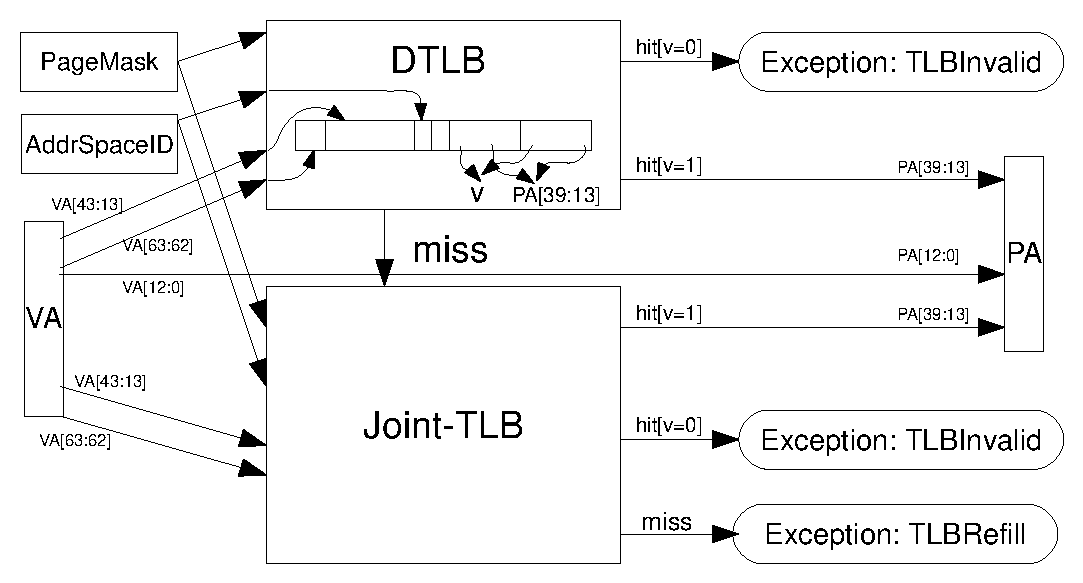
\includegraphics[width=0.8\textwidth]{4.analysis/mips_addrtrans}\\
  \caption{Трансляция адреса в MIPS}\label{fig:mips_address_translation}
\end{figure}


В зависимости от значения виртуального адреса и состояния управляющих регистров
возможны следующие варианты трансляции адреса:
\begin{itemize}
  \item для виртуального адреса трансляция проходит через TLB
(см.рис.~\ref{fig:mips_address_translation});
  \item для виртуального адреса трансляция проходит без таблиц (физический адрес
--- битовая строка --- является результатом битовых операций над виртуальным
адресом --- битовой строкой).
\end{itemize}

Пример модели инструкции LD с рисунка~\ref{fig:mips64_page} приведен в приложении~\ref{sec:xml}.

\section{Генерация тестов для архитектуры PowerPC}

Архитектура PowerPC разработана компанией IBM. Документация по архитектуре
PowerPC представлена в PowerPC Architecture Book (в трех томах)~\cite{PowerPC}. Первый том (PowerPC User Instruction Set Architecture) содержит описания инструкций, которые действительно описываются в виде набора операций над битовыми строками (см.рис.~\ref{fig:ppc_page}.

\begin{figure}
\textbf{Store Halfword Indexed X-form}

sthx RS,RA,RB

\begin{verbatim}
if RA = 0 then b <- 0
else           b <- (RA)
EA <- b + (RB)
MEM(EA, 2) <- (RS)48:63
\end{verbatim}

Let the effective address \texttt{(EA)} be the sum \texttt{(RA|0)+(RB)}. \texttt{(RS)48:63} are stored into the halfword in storage addressed by \texttt{EA}.\\

\textbf{Special Registers Altered:}\\
None
\caption{Пример страницы документации системы команд PowerPC}\label{fig:ppc_page}
\end{figure}

Третий том (PowerPC Operating Environment Architecture) содержит описание подсистемы управления памяти в микропроцессорах PowerPC. Для работы с данными она содержит следующие блоки (количественные характеристики приведены для микропроцессора PowerPC 970FX
~\cite{PowerPC970FXUserManual}):
\begin{itemize}
  \item \emph{кэш-память данных первого уровня (D-Cache-1)}:
        \begin{itemize}
            \item размер: 32 кБ;
            \item поля строк: тэг физического адреса (ключ), данные (данные);
            \item битовая длина номера региона: 7 (наборно-ассоциативная
кэш-память);
            \item количество строк в регионе: 2;
            \item стратегия вытеснения \LRU;
        \end{itemize}
  \item \emph{кэш-память второго уровня (Cache-2)}:
        \begin{itemize}
            \item размер: 512 кБ;
            \item поля строк: тэг физического адреса (ключ), данные (данные);
            \item битовая длина номера региона: 11 (наборно-ассоциативная
кэш~--~память);
            \item количество строк в регионе: 8;
            \item стратегия вытеснения \LRU;
        \end{itemize}
  \item \emph{D-TLB} (кэш таблицы страниц):
        \begin{itemize}
            \item поля строк: номер страницы виртуальной памяти (ключ), номер
фрейма физической памяти (данные);
            \item битовая длина номера региона: 8 (наборно-ассоциативный);
            \item количество строк в регионе: 4;
            \item стратегия вытеснения \LRU;
        \end{itemize}
  \item \emph{сегментные регистры (SLB, Segment Lookaside Buffer)}:
        \begin{itemize}
            \item поля строк: effective segment id (ключ), virtual segment id
(данные), биты K$_s$/K$_p$, V, N, L, C (данные);
            \item битовая длина номера региона: 0 (полностью ассоциативный);
            \item количество строк в регионе: 64;
            \item вытеснение программное;
        \end{itemize}
        используются для получения виртуального адреса по эффективному;
%  \item \emph{буфер непосредственной трансляции адресов (D-ERAT)}:
% НЕТ ЭТОГО БУФЕРА В АРХИТЕКТУРЕ!!! его добавили в самом микропроцессоре
% PPC970FX
%        \begin{itemize}
%            \item поля строк: номер <<эффективной страницы>> (ключ), номер
% фрейма физической памяти (данные), биты (данные);
%            \item битовая длина номера региона: 6 (наборно-ассоциативная
% таблица);
%            \item количество строк в регионе: 2;
%            \item стратегия вытеснения \FIFO;
%        \end{itemize}
\end{itemize}

Кроме того, в оперативной памяти организуется \emph{таблица страниц виртуальной
памяти (PageTable)}. Хотя формально она не является блоком микропроцессора, но
используется при трансляции адреса, то она тоже может быть оформлена в виде
такой таблицы:
    \begin{itemize}
        \item поля строк: номер страницы виртуальной памяти (ключ), номер фрейма
физической памяти (данные);
        \item битовая длина номера региона: 65;
        \item количество строк в регионе: 1;
        \item вытеснение программное;
        \item размер эффективного адреса: 64 бита;
        \item размер виртуального адреса: 65 бит;
        \item размер физического адреса: 42 бита;
    \end{itemize}

На самом деле таблица страниц виртуальной памяти организована в виде сложной
хэш-таблицы, но для тестирования этот момент не важен --- главное, что это
соответствие номеров страниц виртуальной памяти номерам фреймов физической
памяти, причем необязательно представлены все страницы виртуальной памяти.

Другие блоки для обращения в память не используются.

Осталось показать, что трансляция адреса также может быть представлена в виде
отношений на битовых строках и обращениях в таблицы. Обычное выполнение
обращения к памяти в PowerPC следующее:
\begin{enumerate}
    \item аргументы инструкции обращения к памяти формируется \emph{эффективный
адрес} (EA);
    \item заменой номера сегмента из эффективного адреса получается
\emph{виртуальный адрес} (VA);
    \item заменой номера виртуальной страницы в виртуальном адресе на номер
фрейма физической памяти получается \emph{физический адрес} (PA);
    \item по физическому адресу, если нужно, осуществляется обращение в
кэш-память иди, если данных по физическому адресу нет в кэш-памяти, обращение в
оперативную память.
\end{enumerate}

В зависимости от состояния управляющих регистров возможны следующие варианты
трансляции адреса:
\begin{itemize}
  \item real addressing mode (трансляция выключена); физический адрес
вычисляется по эффективному без обращения к каким-либо таблицам;
  \item режим с трансляцией адреса (см. рис.~\ref{fig:ppc_address_translation}).
\end{itemize}

\begin{figure}[h] \center
  \includegraphics[width=\textwidth]{4.analysis/ppc_addrtrans}\\
  \caption{Трансляция адреса в PowerPC}\label{fig:ppc_address_translation}
\end{figure}


\section{Генерация тестов для архитектуры IA-32}

IA-32 --- это архитектура, разрабатываемая компанией Intel. Документация по
архитектуре IA-32 представлена книгой IA-32 Intel® Architecture
Software Developer’s Manual (в пяти томах)~\cite{IA32}. Второй и третий тома \\(Instruction Set Reference) содержат определения инструкций, которые действительно описываются в виде набора операций над битовыми строками (см.рис.~\ref{fig:ia32_page}).

\begin{figure}
\textbf{TEST—Logical Compare}\\

\textbf{Description}\\
Computes the bit-wise logical AND of first operand (source 1 operand) and the second operand
(source 2 operand) and sets the SF, ZF, and PF status flags according to the result. The result is
then discarded.\\

\textbf{Operation}
\begin{verbatim}
TEMP <- SRC1 AND SRC2;
SF <- MSB(TEMP);
IF TEMP = 0
  THEN ZF <- 1;
  ELSE ZF <- 0;
FI:

PF <- BitwiseXNOR(TEMP[0:7]);
CF <- 0;
OF <- 0;
(* AF is undefined *)
\end{verbatim}

\textbf{Flags Affected}\\
The OF and CF flags are set to 0. The SF, ZF, and PF flags are set according to the result (see
the "Operation" section above). The state of the AF flag is undefined.

\caption{Пример страницы документации системы команд архитектуры IA-32}\label{fig:ia32_page}
\end{figure}

Четвертый и пятый тома (System Programming Guide) содержат описание подсистемы управления памяти в
микропроцессорах IA-32. Для работы с данными она содержит следующие блоки
(количественные характеристики приведены для микропроцессора Intel Pentium
Pro~\cite{PentiumPro}) :
\begin{itemize}
  \item \emph{кэш-память данных первого уровня (D-Cache-1)}:
        \begin{itemize}
            \item размер: 8 кБ;
            \item поля строк: тег адреса (ключ), данные (данные);
            \item битовая длина номера региона: 7 (наборно-ассоциативный);
            \item количество строк в регионе: 2;
            \item стратегия вытеснения \LRU;
        \end{itemize}

  \item \emph{кэш-память второго уровня (Cache-2)}:
        \begin{itemize}
            \item размер: в разных версиях 256 кБ, 521 кБ или 1 МБ;
            \item поля строк: тег адреса (ключ), данные (данные);
            \item битовая длина номера региона: от 11 до 13 в разных версиях
(наборно-ассоциативный);
            \item количество строк в регионе: 4;
            \item стратегия вытеснения \LRU;
        \end{itemize}

  \item \emph{TLB (D-TLB)}:
        \begin{itemize}
            \item поля строк: page number (ключ), page base address (данные),
флаги (данные);
            \item битовая длина номера региона: 4 (наборно-ассоциативный);
            \item количество строк в регионе: 4;
            \item стратегия вытеснения \LRU;
        \end{itemize}

  \item \emph{таблица страниц виртуальной памяти (PageTable)}:
    \begin{itemize}
        \item поля строк: page number (ключ), page base address (данные), флаги
(данные);
        \item битовая длина номера региона: 65;
        \item количество строк в регионе: 1;
        \item вытеснение программное;
        \item размер логического адреса: 48 бит;
        \item размер линейного адреса: 32 бит;
        \item размер физического адреса: 32 бита;
    \end{itemize}


  \item \emph{таблица дескрипторов сегментов (SDT)}:
        \begin{itemize}
            \item поля строк: segment selector (ключ), база (данные), флаги
(данные);
            \item битовая длина номера региона: 13;
            \item количество строк в регионе: 1;
            \item вытеснение программное;
        \end{itemize}
\end{itemize}

Другие блоки для обращения в память не используются.

\begin{figure}[h] \center
  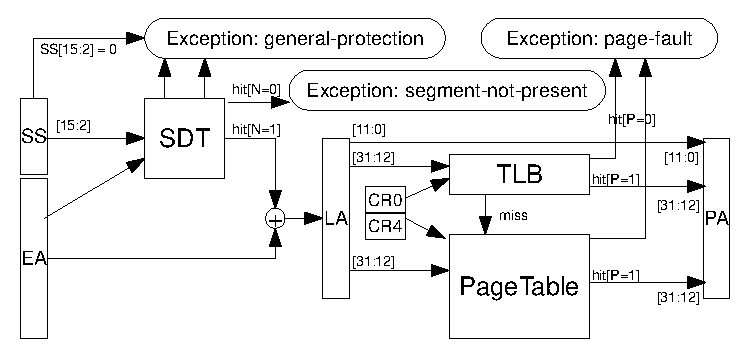
\includegraphics[width=0.8\textwidth]{4.analysis/ia32_addrtrans}\\
  \caption{Трансляция адреса в IA-32}\label{fig:ia32_address_translation}
\end{figure}

Осталось показать, что трансляция адреса также может быть представлена в виде
отношений на битовых строках и обращениях в таблицы. Обычное выполнение
обращения к памяти в IA-32 следующее:
\begin{enumerate}
    \item аргументы инструкции обращения к памяти формируется \emph{логический
адрес} (SS:EA);
    \item заменой номера сегмента из логического адреса получается
\emph{линейный адрес} (LA);
    \item либо линейный адрес трактуется как физический, либо заменой номера
виртуальной страницы в линейном адресе на номер фрейма физической памяти
получается физический адрес (PA);
    \item по физическому адресу, если нужно, осуществляется обращение в
кэш-память иди, если данных по физическому адресу нет в кэш-памяти, обращение в
оперативную память.
\end{enumerate}

В зависимости от состояния управляющих регистров возможны следующие варианты трансляции адреса:
\begin{itemize}
  \item real-address mode (трансляция выключена) --- физический адрес равен линейному, линейный адрес вычисляется по логическому без обращения к каким-либо таблицам;
  \item protected mode --- режим с трансляцией адреса через таблицу страниц (см. рис.~\ref{fig:ia32_address_translation}).
\end{itemize}



\section{Реализация}

Реализация генератора программ состоит из компонентов, представляющих следующие <<деятельности>> (см. рис.~\ref{fig:activities}):
\begin{figure}[h] \center
  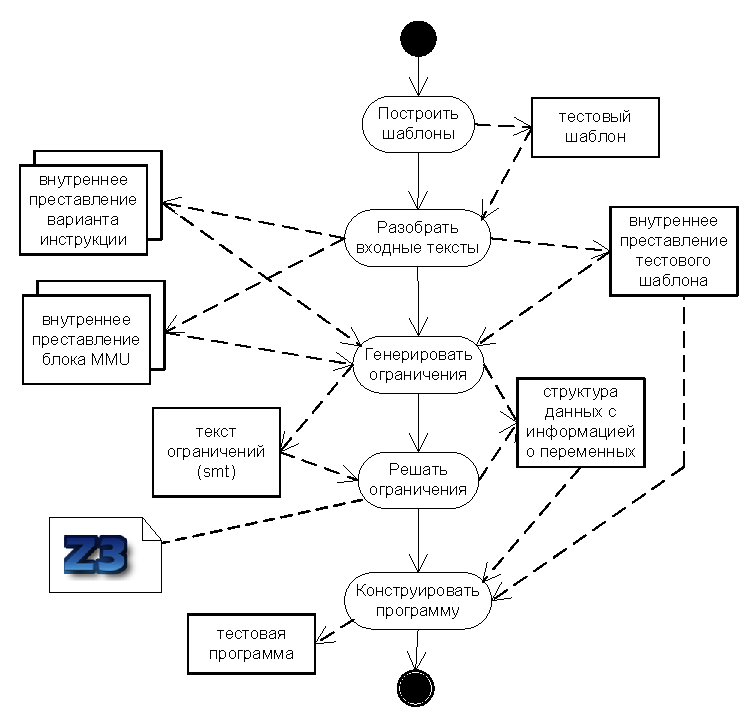
\includegraphics[width=0.7\textwidth]{3.impl/activities1}\\
  \caption{Диаграмма деятельностей по генерации тестовых программ}\label{fig:activities}
\end{figure}
\begin{enumerate}
  \item генерация тестовых шаблонов;
  \item синтаксический анализ исходных текстовых данных; создается внутреннее представление шаблона, моделей блоков, моделей вариантов инструкций для других компонентов;
  \item генерация (текстов) ограничений с использованием описанных в разделах~\ref{sec:constraints_generation_section} и \ref{sec:usefulness_functions} методов (smt~\cite{SMT}); кроме того строится структура, хранящая семантическую информацию о созданных переменных в ограничениях;
  \item обертка решателя ограничений; вызывается внешний решатель ограничений, берется результат его работы, извлекаются из него значения переменных и эти значения прописываются в созданной ранее структуре;
  \item конструирование текстов программ на основе внутреннего представления шаблона и значениях переменных.
\end{enumerate}

Реализация для модельного микропроцессора архитектуры MIPS64~\cite{mips64II} включала следующие компоненты:
\begin{itemize}
  \item генератор тестовых шаблонов внешний --- MicroTESK~\cite{MicroTESK};
  \item решатель ограничений внешний --- Z3~\cite{Z3};
  \item синтаксический анализ моделей, генерация текстов ограничений, обертка решателя ограничений --- компонент <<Генератор ограничений>> на Ruby (порядка 2000 строк);
  \item конструирование тестовых программ --- компонент на Java (порядка 500 строк).
\end{itemize}

Типичный размер модели варианта инструкции --- 100 строк (в представлении на xml). Типичный размер модели блока --- 20 строк (в представлении на xml).

Генератор ограничений практически целиком переносим при смене архитектуры.

\section{Оценка допустимой сложности тестовых\\шаблонов}\label{sec:templates_estimation}

%эксперименты с длинами и временем генерации/процентом успешной
%генерации. Показать, что допустимая длина действительно увеличивается!

Был реализован прототип генератора ограничений для модельного микропроцессора архитектуры
MIPS64~\cite{mips64II}. В качестве решателя ограничений в нем использовался Z3~\cite{Z3}. Был проведен ряд экспериментов. Целью этих экспериментов было исследование допустимой сложности тестовых шаблонов при использовании предлагаемых в диссертации методов (под сложностью понимается
качество шаблона, пропорциональное количеству зависимых данных в нем).

В экспериментах тестовые шаблоны состояли из инструкций загрузки и сохранения
данных в памяти. В каждой инструкции должна была выполняться трансляция адреса
через TLB (с использованием D-TLB) и затем обращение в основную память через
кэш-память первого уровня. Рассматривались все длины тестовых шаблонов от 2 до
16. Для каждой длины рассматривались следующие ассоциативности кэш-памяти --- 2,
4, 8 и 16. При фиксированной длине шаблона и ассоциативности кэш-памяти
случайным образом генерировался тестовый шаблон (более конкретно, зависимости
аргументов инструкций).

Рисунки~\ref{fig:success_experiment} и~\ref{fig:time_experiment} представляют
некоторые средние значения (среднее бралось по всем тестовым шаблоном
фиксированной длины). На рисунке~\ref{fig:success_experiment} отражена доля
шаблонов, для которых был построен тест за время, меньшее чем 60 секунд (если
время превышало 60 секунд, построение теста обрывалось). На
рисунке~\ref{fig:time_experiment} отражено среднее время генерации теста (по
сути, среднее время разрешения ограничений). Более точно, среднее время
продуктивного принятия решения о тестовом шаблоне, т.е. время определения того,
что шаблон является несовместным (для него не может быть теста вовсе) или
совместным с построением теста.

Эксперименты проходили на компьютере AMD Athlon64 3200+ 2ГГц с 1ГБ оперативной
памяти.

\begin{figure}[p] \center
\parbox[t]{\textwidth}{
  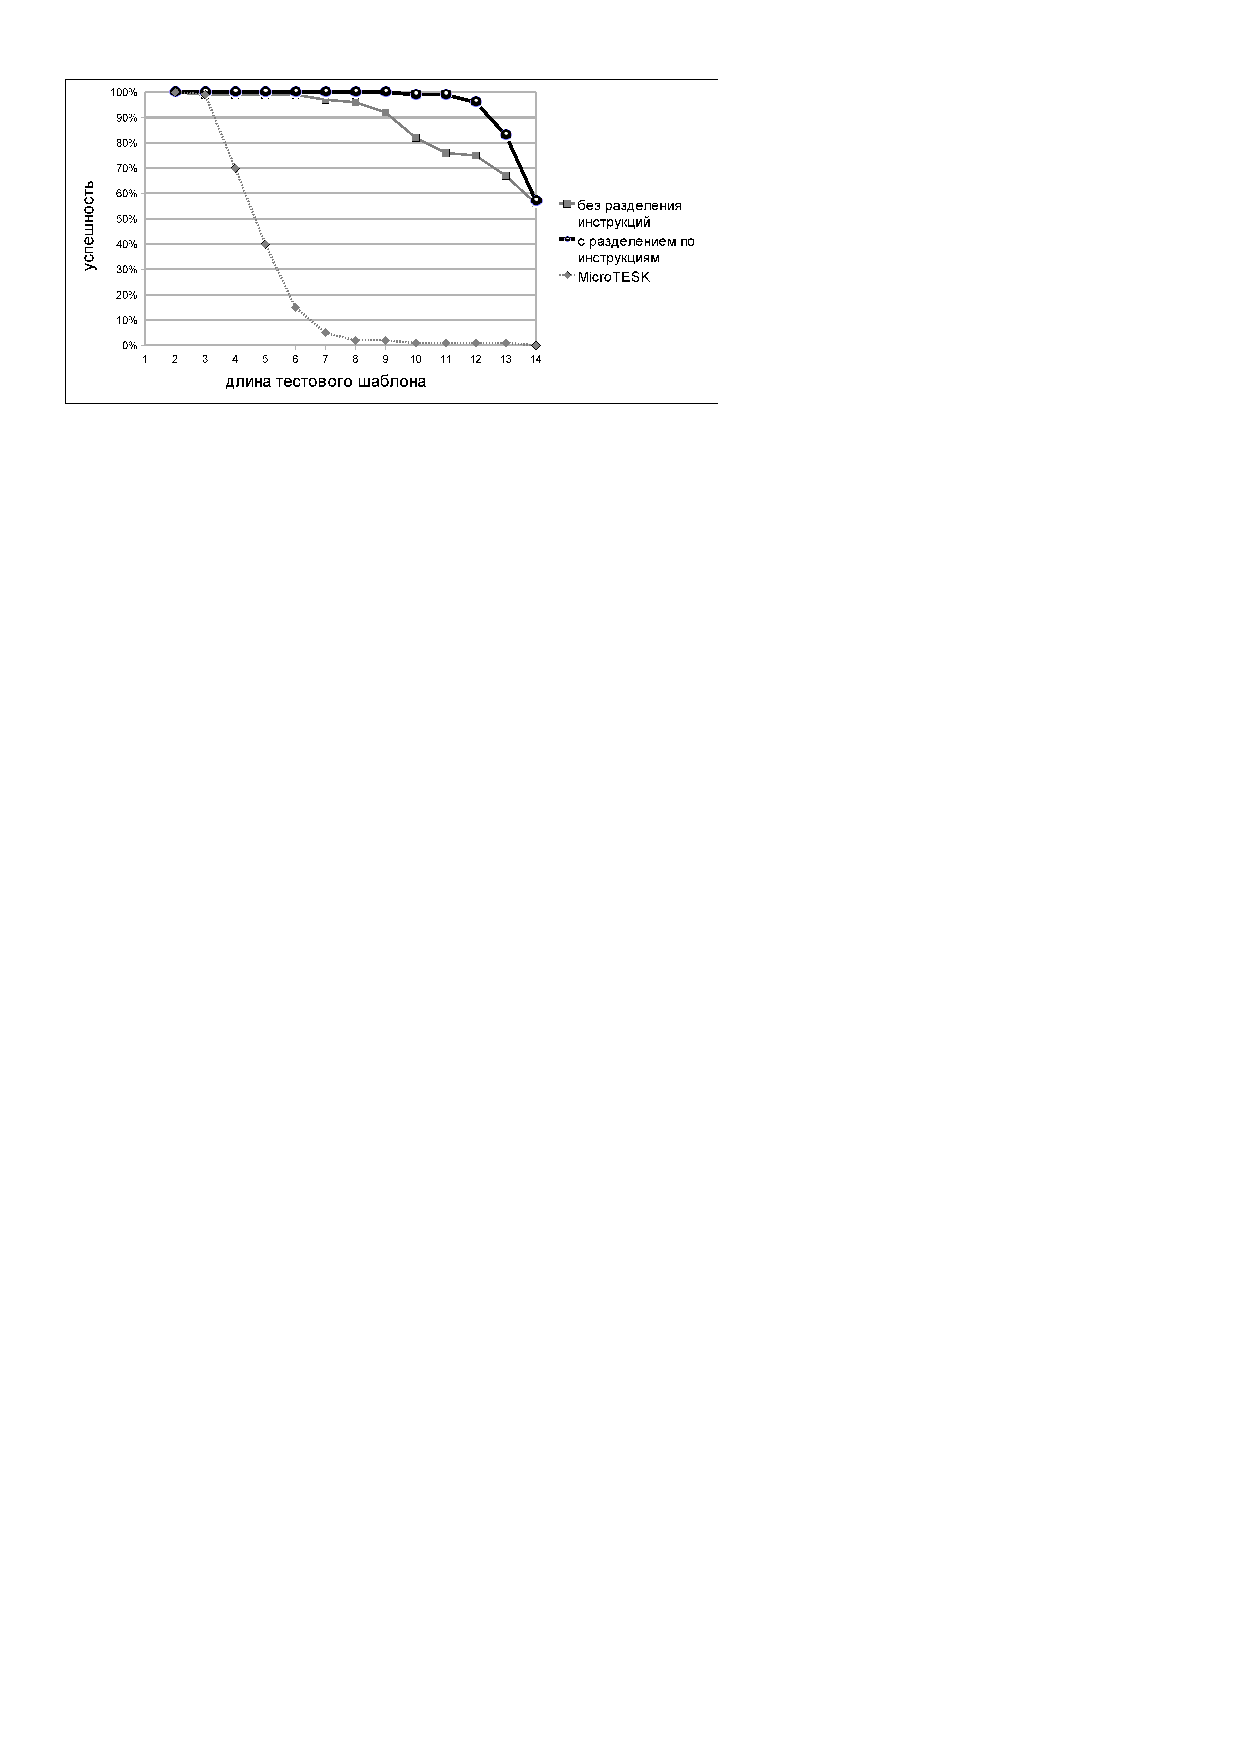
\includegraphics[width=\textwidth]{4.analysis/success_exprmnt}%
\caption{Доля тестовых шаблонов, для которых удалось построить тест за 60с или
определить их несовместность}\label{fig:success_experiment}
}

\vspace{1.5cm}

\parbox[t]{\textwidth}{
  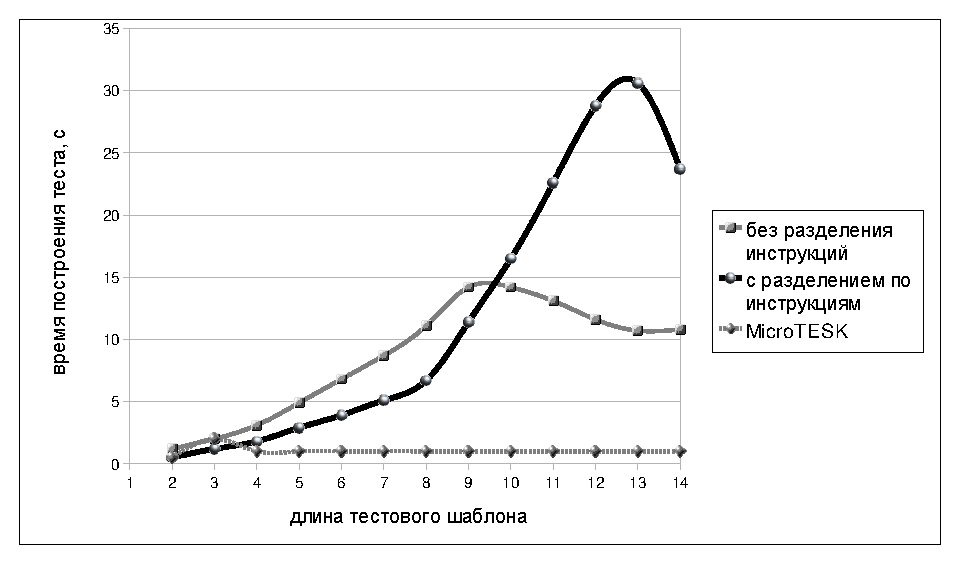
\includegraphics[width=\textwidth]{4.analysis/time_exprmnt}
  \caption{Среднее время продуктивного принятия решения о тестовом
шаблоне}\label{fig:time_experiment}
}
\end{figure}

В первой серии экспериментов (их результаты отражены на рисунках линиями с
квадратиками) генерация ограничений делалась для всего тестового шаблона.
Оказалось, что до некоторой длины шаблона (значит, и теста) (8-9) метод работает
успешно практически для всех тестовых шаблонов (97\%-100\%). При дальнейшем
увеличении длины шаблона начинает уменьшаться доля шаблонов, для которых удается
построить тест (по 5-10\% при увеличении длины теста). Тем самым при длине теста
порядка 14-15 уже для половины шаблонов решатель ограничений не успевает за 60
секунд принять решение и построить тест. В результате анализа использованных в
экспериментах тестовых шаблонов был сделан вывод, что для большинства из них
(60-70\%) тестов не может быть вовсе, так как в этих шаблонах имеются обращения
по одинаковым адресам с кэш-промахами после кэш-попаданий и кэш-промахами после
кэш-промахов (поскольку в результате кэш-промаха данные помещались в кэш-память
и при повторном обращении к ним должно происходить только кэш-попадание, а не
кэш-промах).

Поскольку эта ситуация стала по сути следствием случайного выбора тестовых
шаблонов, то в следующей серии экспериментов перед запуском генерации
ограничений была вставлена процедура, отсеивающая априори несовместные тестовые
шаблоны (т.е. такие, для которых не может существовать тестов вовсе). Кроме того
обращения в кэш-память были поделены на группы на основе одинаковых имен
аргументов и для этих групп генерировались ограничения (грубо говоря, к шаблону
добавлялось требование обращения по разным именам аргументов в разные регионы,
если это не противоречило шаблону). Результаты этой второй серии экспериментов
отражены на рисунках~\ref{fig:success_experiment} и \ref{fig:time_experiment}
линией с кружками. Из них следует, что примененные изменения позволили
дополнительно увеличить на несколько единиц допустимый размер тестового шаблона.

Для каждой пары (длина шаблона, ассоциативность) было сгенерировано 1000
тестовых шаблонов. Насколько можно доверять полученным в экспериментах
результатам на таком количестве тестовых шаблонов? Для ответа на этот вопрос воспользуемся аппаратом теории
вероятностей. Пусть $N$ --- количество испытаний. Одно испытание заключается в
следующем: сначала случайным образом строится тестовый шаблон, затем генерируются
для него ограничения и, наконец, они разрешаются. Испытание заканчивается успешно, если за отведенное время (60с) решатель ограничений построил тест, и неуспешно, если не успел построить.
Обозначим  $\xi_i$, $i = 1, 2, \dots, N$, случайные величины, соответствующие
успешности испытаний. Их областью значений будет множество $\{0, 1\}$. Эти
случайные величины независимы и одинаково распределены (обозначим $p =
\mathsf{P}\{\xi_i = 1\}$). Поэтому применим \emph{закон больших чисел}, согласно
которому $\frac{\sum_{i=1}^N \xi_i}{N} ~ p$ при <<больших>> $N$. Более точно, для любых
положительных $\varepsilon$ и $\delta$ найдется число $N^*$, что для всех $N > N^*$ будет
выполнено $\mathsf{P}\{|\frac{\sum_{i=1}^N \xi_i}{N} - p | \geq \varepsilon\} \leq \delta$. $\varepsilon$ --- это допустимое отклонение в оценке результата экспериментов (т.е. оценке $p$). $\delta$ показывает, насколько можно доверять полученному результату экспериментов. Поскольку $\sum \xi_i$ распределена по биномиальному закону ($\mathsf{P}\{\sum_{i=1}^N \xi_i = m\} = \binom{N}{m} p^m (1{-}p)^{N{-}m}$), то для вероятности отклонения более, чем на $\varepsilon$, справедлива следующая формула: $$\sum_{m = 0}^{(p-\varepsilon)N} \binom{N}{m} p^m (1{-}p)^{N{-}m} + \sum_{m = (p+\varepsilon)N}^N \binom{N}{m} p^m (1{-}p)^{N{-}m} \leq \delta$$ Эта формула позволяет оценить $\delta$ при разных $p$, зная $\varepsilon$ и $N$.

Итак, для каждого $n \in \{2,3\}$ ($n$ --- длина тестового шаблона) было сгенерировано по $B = 1000$ тестовых шаблонов. При этом получилось $p \in [0.9, 1.0]$. Если взять допустимое отклонение от истинного значения $\varepsilon = 0.02$ (2\%) (что вполне допустимо, т.к. отклонение в 2\% не сильно изменит результат эксперимента), то вероятность ошибиться в этом случае была бы не более $\delta = 0.03$, т.е. 3\%, что тоже вполне допустимо. Для $n \in \{4, 5, 6, 7\}$ было сгенерировано по $N = 2000$ тестовых шаблонов (для $w \in \{2,4\}$). Если взять $\varepsilon = 0.02$ (2\%), то для $p \in [0.9, 1.0] \delta = 0.003$, т.е. $0.3\%$, т.е. ошибка в этом случае еще меньше. И, наконец, для $n \in \{8, 9, ..., 14\}$ было сгенерировано по $N = 3000$ тестовых шаблонов, что при $\varepsilon = 0.02$ и $p \in [0.5, 1.0]$ дает $\delta = 0.02$, т.е. всего 2\%. Таким образом, вероятность ошибки в проведенных экспериментах невелика.

Проведенные эксперименты позволяют произвести сравнение с инструментом
MicroTESK~\cite{MicroTESK}. Этот инструмент был успешно применен для построения
тестов по всевозможным тестовым шаблонам из 2-3 инструкций~\cite{vorobyev}. При
увеличении длины тестового шаблона (и, соответственно, сложности) удается
строить тесты для всё меньшего количества шаблонов. Что и отражено на
рисунках~\ref{fig:success_experiment} и \ref{fig:time_experiment} линиями с
ромбами. Напротив, как показывают эксперименты, предложенные методы позволяют
строить тесты по шаблонам из 8-11 инструкций обращения к памяти. Допустимая
длина шаблонов может быть еще больше, если кроме инструкций обращения к памяти в
шаблоне используются и другие инструкции (например, арифметические).

\section{Сравнение с Genesys-Pro}

В прошлом разделе было произведено сравнение с инструментом\\
MicroTESK~\cite{MicroTESK}. В этом разделе будет произведено сравнение с другим
инструментом нацеленной генерации тестов --- Genesys-Pro~\cite{GenesysPro}. Сравнить
по эффективности и провести эксперименты с Genesys-Pro не удается, поскольку
этот инструмент не распространяется за пределы IBM. Однако имеется ряд
публикаций~\cite{GenesysPro2004Innovations, GenesysSolver}, на основе которых удалось сделать некоторое сравнение.

Технологически генерация тестов с использованием Genesys-Pro выглядит следующим
образом:
\begin{enumerate}
    \item подготовить Architectural simulator --- эталонный симулятор
микропроцессора;
    \item подготовить Architectural model --- описание системы команд
тестируемого микропроцессора с указанием для каждой инструкции набора атрибутов
и ограничений значений атрибутов (по сути, описание в виде ограничений
предусловий инструкций и вычисляемым им функций); пример описания инструкции
LoadWord изображен на рисунке~\ref{fig:GenesysProArchitecturalModel}; для
описания трансляции адреса предлагается метод DeepTrans~\cite{DeepTrans} ---
пример изображен на рисунке~\ref{fig:DeepTransExample};
    \item подготовить Test template --- тестовый шаблон; в нем задаются
инструкции теста и интересные для тестирования ситуации исполнения инструкций;
    \item подготовить Testing knowledge --- комплект ограничений на аргументы
инструкций, описывающих ситуации исполнения инструкций из test template;
    \item подготовить или использовать имеющийся решатель ограничений;
    \item запустить Genesys-Pro с подготовленными моделями.
\end{enumerate}
%% я понимаю, что такую последовательность шагов нельзя называть
%% технологической, ибо непоятно
%% 1) как выбирать Testing knowledge - что туда включать, а что нет; наверняка,
%% есть некое понимание того, что хочется протестировать; это понимание
%% должно быть формализовано (модель покрытия) и на его основе уже решать,
%% что включать в Testing knowledge, а что нет;
%% 2) не описано, как анализировать результаты Genesys-Pro: всё ли он сделал или
%% нет, надо ли дорабатывать то, что он генерирует? Надо ли как-то иначе
%% формулировать модели с шагов 1-3 для того, чтобы тесты были построены
%% целиком. И что значит "целиком"? Нет ведь модели покрытия!

\begin{figure}[h] \center
  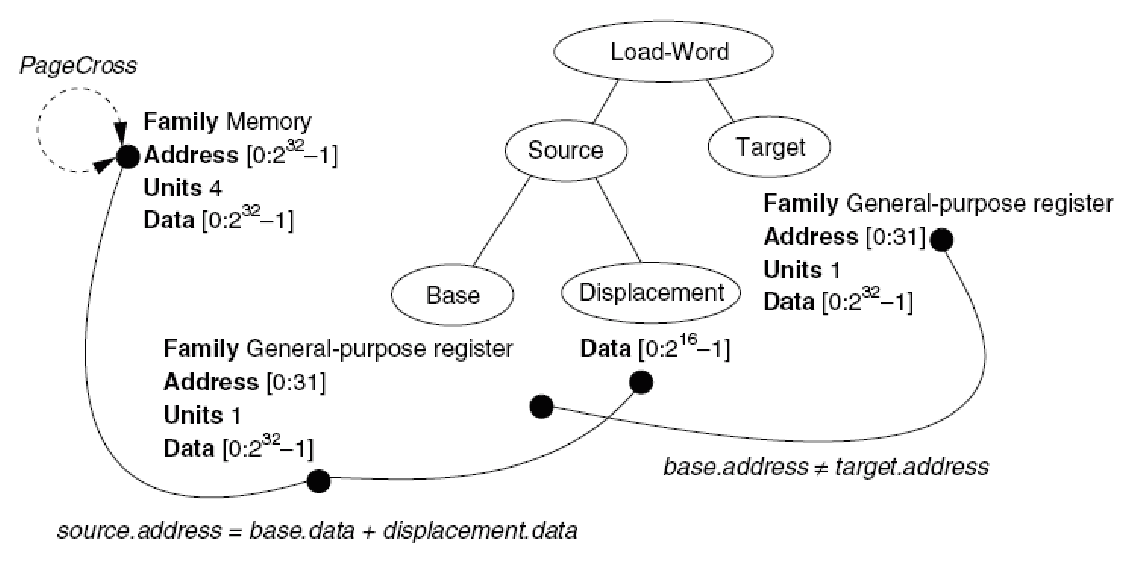
\includegraphics[width=0.8\textwidth]{4.analysis/arch-model}
  \caption{Architectural model для инструкции
LoadWord}\label{fig:GenesysProArchitecturalModel}
\end{figure}

\begin{figure}[h] \center
  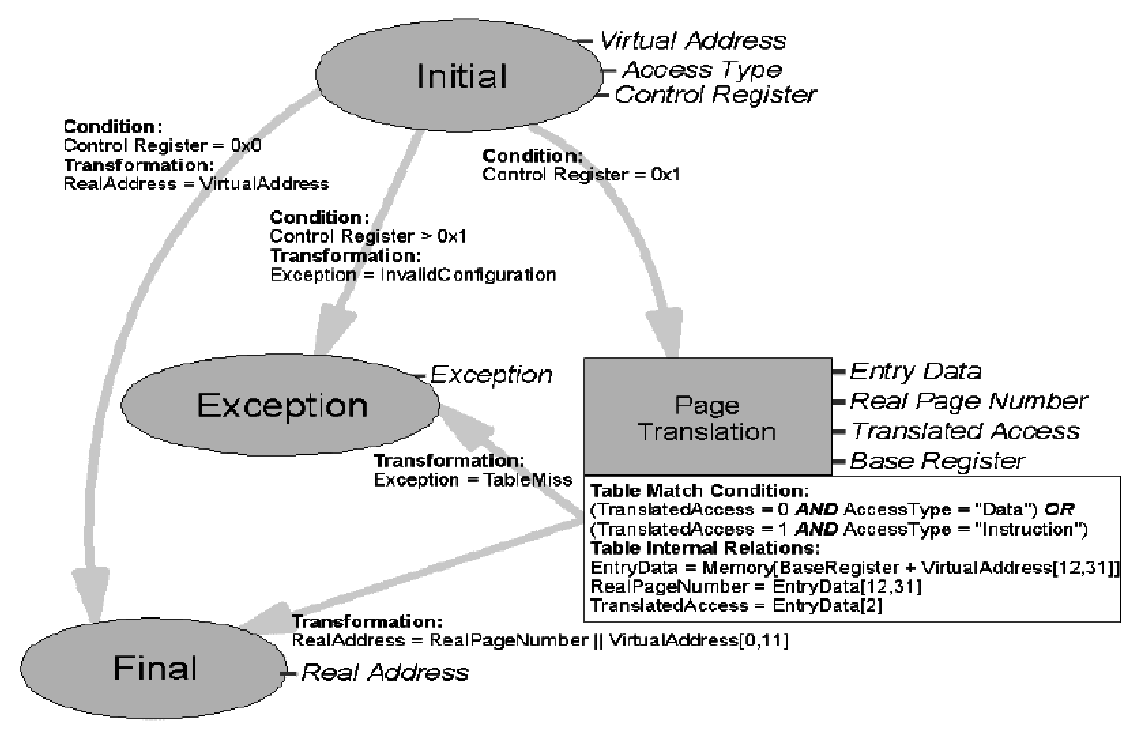
\includegraphics[width=0.8\textwidth]{4.analysis/deeptrans}
  \caption{Пример трансляции адреса в DeepTrans}\label{fig:DeepTransExample}
\end{figure}

\begin{figure}[h] \center
  \includegraphics[width=\textwidth]{4.analysis/g-pro}
  \caption{Genesys-Pro (слева) и предлагаемый в диссертации генератор
(справа)}\label{fig:GenesysProScheme}
\end{figure}

Genesys-Pro работает следующим образом: (см. левую часть
рис.~\ref{fig:GenesysProScheme})
\begin{enumerate}
    \item выбирает очередную инструкцию из Test template, для нее запрашивает
определение из Architectural model и для указанной для нее тестовой ситуации
запрашивает определение из Testing knowledge; кроме того запрашивает текущее
состояние микропроцессора у Architectural simulator;
    \item составляет из этого систему ограничений, передает их для разрешения на
costraint solver и получает ответ;
    \item формирует инструкцию и записывает ее в Test program, а также формирует
часть начального состояния (initial state);
    \item исполняет инструкцию на Architectural simulator, тот ее исполняет.
\end{enumerate}
% т.е. получается, симулятор должен быть каким-то особенным, чтобы уметь
% работать из неполного состояния? (с lazy-значениями 'X') поскольку не
% всё начальное состояние построено перед
% первой инструкций и достраивается в процессе построения теста

\paragraph{Сходства с Genesys-Pro} следующие:
\begin{itemize}
    \item подход, в котором тестовый шаблон и микропроцессор описываются
декларативным образом, и кроме этого есть независимый от них генератор, который
принимает на вход эти описания и строит тест; альтернативным решением могла быть
технология, в которой по модели вручную приходилось бы создавать дополнительные
исполнительные модули, учитывающие особенности модели микропроцессора и
тестового шаблона;
    \item использование ограничений (constraints) для построения тестов;
    \item сходные идеи есть и в методе описания трансляции адресов: Genesys-Pro
предлагает декларативное описание, в котором описываются разные варианты
трансляции с указанием того, как формируются виртуальные/физические адреса, и в
предлагаемом в диссертации подходе описывается формирование адресов; и там, и
там речь идет о \emph{таблицах}, для которых формулируются атрибуты (в том числе
и предикат типа keyMatch).
\end{itemize}

\paragraph{Отличия от Genesys-Pro} следующие:
\begin{itemize}
    \item разные принципы построения ограничений; Genesys-Pro строит тест по
одной инструкции и формулирует ограничения только для одной очередной
инструкции; напротив, в предлагаемом методе ограничения строятся для всего
тестового шаблона целиком;
    \item разные методы построения ограничений; Genesys-Pro знает всё состояние
микропроцессора целиком при формулировании ограничения на очередную инструкцию;
напротив, в предлагаемом методе ограничения состояние микропроцессора неизвестно
вообще; это приводит к ограничениям разной природы;
    \item Genesys-Pro предполагает для инструкции раздельное описание
вычисляемой функции и ограничений на входные данные; в предлагаемом методе эти
описания оформляются вместе;
    \item Genesys-Pro позволяет компактно описать длинные тесты, но важно то,
что эти возможности позволяют описывать целые классы последовательностей
инструкций;
    \item разный способ описания инструкций; Genesys-Pro предлагает делать это в
виде ограничений на атрибуты инструкции, а здесь --- в виде цепочки операторов;
    \item Genesys-Pro рассчитан на подготовку специальных решателей ограничений;
напротив, в предлагаемом методе используются сторонние решатели ограничений и
отдельно подготавливать их не нужно.
\end{itemize}

\paragraph{Преимущества и недостатки по сравнению с Genesys-Pro}:
\begin{itemize}
    \item с помощью Genesys-Pro удается строить очень длинные тесты, но не обязательно эти тесты будут сложными (иметь большое количество зависимых данных);
    \item существует тестовый шаблон, для которого существует тест, но Genesys-Pro его не построит за некоторое время (без, возможно, неописанных в публикациях эвристик), а предлагаемым в диссертации методом тест будет построен; в этом тестовом шаблоне последовательность инструкций должна быть фиксирована; а возможный пример ситуаций в шаблоне такой: в одной из инструкций должны быть вытеснены некоторые специальные данные, которых нет в текущем состоянии из-за неверного выбора данных для предыдущих инструкций;
    \item тем не менее, возможное отсутствие фиксированной цепочки дает Genesys-Pro бонус, поскольку при наличии выбор инструкции может быть успешно сделан с учетом текущего состояния микропроцессора;
    \item Genesys-Pro приходится работать с большими массивами данных (это память, всевозможные кэши и таблицы страниц), эти массивы данных участвуют в ограничениях; поэтому в решателе ограничений приходится разрабатывать методы эффективной работы с ними~\cite{GenesysSolver}; задача построение такого решателя обладает высокой сложностью (как и задача построения эффективного решателя ограничений вообще); кроме того, большая часть такого решателя может оказаться невостребованной при работе с другой моделью микропроцессора, с другим классом тестовых шаблонов --- его придется писать заново; а в предлагаемом методе разрабатывать собственные решатели не нужно.
\end{itemize}

%Genesys-Pro чётко разделяет свойства аргументов
%инструкции и свойства результата инструкции, соотношение между ними
%задается не с помощью ограничений (т.е. не декларативным способом),
%а в виде алгоритма (т.е. императивным способом).
%
%Другой особенностью Genesys-Pro является то, что поддерживаемые им
%тестовые шаблоны зачастую не фиксируют последовательность инструкций
%(это позволяет строить более простые ограничения, потому как
%генерируемая последовательность инструкций может по ходу генерации
%подстраиваться под уже сгенерированные инструкции со
%сгенерированными значениями аргументов, под состояние
%микропроцессора, в которое привели сгенерированные инструкции).
%
%Выразительный язык Genesys-Pro для описания ограничений однако
%содержит такие нетривиальные конструкции, как явное использование
%элементов массивов данных, что требует для разрешения продвинутый
%решатель CSP, в том числе и заточенный под особенности генерации
%тестовых данных для тестовых шаблонов (как минимум такие ограничения
%могут включать битовые операции). Подобный решатель был разработан в
%IBM для инструмента Genesys-Pro~\cite{GenesysSolver}. Однако
%создание такого решателя -- отдельное сложное исследование, которое
%не входило в цели данного исследования. В данной работе было принято
%решение использовать доступные существующие решатели (не обязательно
%CSP) и сосредоточиться на упрощении генерируемых ограничений для
%некоторых частных случаев архитектур.
%
%%\begin{figure}[h]
%%\parbox{0.5\textwidth}{ \centering
%%  \includegraphics[width=0.45\textwidth]{3.impl/genesys-pro}
%%} \vline
%%\parbox{0.5\textwidth}{ \centering
%%  \includegraphics[width=0.45\textwidth]{3.impl/mygen}
%%}
%%\caption{Сравнение с Genesys-Pro}\label{comparison_genesyspro}
%%\end{figure}
%
%В отличие от Genesys-Pro в предлагаемом инструменте описание
%семантики инструкций задается в едином виде -- в виде описаний
%тестовых ситуаций~\cite{my_syrcose_2008, my_isp_2008}. Каждая
%тестовая ситуация описывает не только ограничение на свои аргументы,
%но и результат исполнения инструкции \emph{при данном ограничении на
%аргументы} инструкции декларативным образом. В функции, которую
%реализует инструкция, выделяются отдельные \emph{ветви
%функциональности}, ситуации различного поведения инструкций, каждая
%ветвь функциональности становится отдельной тестовой ситуацией.
%Например, инструкция целочисленного сложения ADD может быть
%исполнена либо точно, либо с возникновением переполнения. Поэтому у
%этой инструкции можно выделить 2 ветви функциональности (точное
%исполнение и исполнение с переполнением), каждая ветвь дает свою
%тестовую ситуацию.

\section{Сравнение с работами Intel}

В ряде публикаций~\cite{MicroFORMAL} описывается инструмент MicroFORMAL, разрабатываемый в Intel. Он используется для некоторых задач формальной верификации разрабатываемых микропроцессоров (в частности, для проверки обратной совместимости). В рамках этой работы требуется описывать поведение микропроцессоров, формализовывать инструкции. Авторы статей упоминают \emph{IRL-представление} микрокода (IRL --- Intermediate Representation Language). Спецификация на IRL описывает функциональность инструкции и побочный эффект (изменение <<внешних>> переменных). Ровно ту же цель преследуют и модели инструкций, предлаагемые в данной работе. Спецификация на IRL представляет собой последовательность операторов (эта же идея используется здесь).

IRL включает в себя управляющие операторы (\texttt{if}, \texttt{goto}), поскольку верификация с использованием спецификаций на IRL нацелена в первую очередь на верификацию потоков управления. В данной работе поток управления не предполагает подобных операторов.

IRL позволяет описывать инструкции обращения к памяти. Однако в нем используется только плоская модель памяти (т.е. память как одномерный массив ячеек) с возможностью обращения <<по индексу>>. Напротив, модели инструкций, предлагаемые в данной работе, позволяют описывать работу с памятью более детально, с указанием успешности обращений в различные блоки подсистемы управления памяти. 


% !Mode:: "TeX:UTF-8"
\chapter*{Заключение}
\addcontentsline{toc}{chapter}{Заключение}

Основные научные и практические результаты, полученные в
диссертационной работе и выносимые на защиту, состоят в следующем:

\Results

%Основные результаты диссертации являются новыми, получены автором самостоятельно.



%% TODO:
%% 1) формальные определения тестового шаблона, ограничения, совместности системы ограничений
%% 4) непроставленные ref чуть ли не с начала theor.tex
%%

\pagebreak
\appendix
% % !Mode:: "TeX:UTF-8"
\chapter{Таблицы ограничений}
%\addcontentsline{toc}{chapter}{Приложение А: Таблицы ограничений}

\begin{table}[h] \small
\begin{tabular}{|c|c|c|c|}
\hline  & \centering случай &
\begin{tabular}{c}переменная\\перебора\end{tabular} & система \\
\hline \hline \multirow{10}{*}{\rotatebox{90}{кэш-попадание}} &
\makecell[c{p{0.3\textwidth}}]{тегсет находится в начальном
состоянии буфера, к нему нет обращений до данной инструкции и он всё
ещё не вытеснен} & $\lambda \in L_0$ &
$\left\{\begin{array}{l} x = \lambda\\
x \notin \{x_1, ..., x_n\}\\
\bigwedge\limits_{x_m:\mbox{miss}}\sum\limits_{i=1}^W v_m(\xi_i) +
\sum\limits^{m-1}_{i=1} u_m(x_i) < W
\end{array}\right.
$ \\ \hhline{~|---} & \makecell[c{p{0.3\textwidth}}]{тегсет
находится в начальном состоянии буфера, к нему есть обращение до
данной инструкции и он всё ещё не вытеснен} & $\lambda \in L_0$ &
$\left\{\begin{array}{l} x = \lambda\\
x \in \{x_1, ..., x_n\}\\
\bigwedge\limits_{x_m:\mbox{miss}}\sum\limits^{m-1}_{i=1} u_m(x_i) <
W
\end{array}\right.
$ \\  \hhline{~|---} & \makecell[c{p{0.3\textwidth}}]{тегсет был
внесен одним из кэш-промахов и с того момента не вытеснен} & -- &
$\left\{\begin{array}{l}
x \in [x_1, ..., x_n]_{miss}\\
\bigwedge\limits_{x_m:\mbox{miss}}\sum\limits^{m-1}_{i=1} u_m(x_i) <
W
\end{array}\right.
$ \\ \hline \hline \multirow{20}{*}{\rotatebox{90}{кэш-промах}} &
\makecell[c{p{0.3\textwidth}}]{тегсет встречается впервые} & -- &
$\left\{\begin{array}{l} x \notin L_0\\
x \notin [x_1, ..., x_n]_{miss}\\
\end{array}\right.
$ \\ \hhline{~|---} & \makecell[c{p{0.3\textwidth}}]{тегсет ранее
был внесен одной из инструкций шаблона, затем вытеснен} & -- &
$\left\{\begin{array}{l}
x \in [x_1, ..., x_n]_{miss}\\
\bigvee\limits_{x_m : \mbox{miss}}\sum\limits^{m-1}_{i=1} u_m(x_i) \geqslant W\\
\end{array}\right.$ \\  \hhline{~|---} &
\makecell[c{p{0.3\textwidth}}]{тегсет находился в начальном
состоянии буфера и был вытеснен, к нему не было обращений в шаблоне}
& $\lambda \in L_0$ & $\left\{\begin{array}{l}
x = \lambda\\
x \notin \{x_1, ..., x_n\}\\
\bigvee\limits_{x_m : \mbox{miss}}\sum\limits^W_{i=1} v_m(\xi_i) + \sum\limits^{m-1}_{i=1} u_m(x_i) \geqslant W\\
\end{array}\right.
$ \\ \hhline{~|---} & \makecell[c{p{0.3\textwidth}}]{тегсет
находился в начальном состоянии буфера и был вытеснен, к нему было
обращение в шаблоне после последнего внесения в буфер} & $\lambda
\in L_0$ &
$\left\{\begin{array}{l} x = \lambda\\
x \in \{x_1, ..., x_n\}\\
\bigvee\limits_{x_m : \mbox{miss}}\sum\limits^{m-1}_{i=1} u_m(x_i) \geqslant W\\
\end{array}\right.
$ \\ \hline
\end{tabular}
\caption{Таблица систем уравнений в случае стратегии вытеснения
\PseudoLRU c использованием функций полезности}\label{plru_table}
\end{table}


\begin{landscape}
\begin{table}[p]\small
\begin{tabular}{|c|c|c|c|c|c|}
\hline  & \centering случай &
\begin{tabular}{c}переменная\\перебора\end{tabular} & система &
\begin{tabular}{c}функция полезности\\для кэш-попадания\end{tabular} &
\begin{tabular}{c}функция полезности\\для кэш-промаха\end{tabular} \\
\hline \hline \multirow{10}{*}{\rotatebox{90}{кэш-попадание}} &
\makecell[c{p{0.38\textwidth}}]{тегсет находится в начальном
состоянии буфера, к нему нет обращений до данной инструкции и он всё
ещё не вытеснен} & $\lambda_\delta \in D$ &
$\left\{\begin{array}{l} x = \lambda_\delta\\
x \notin \{x_1, ..., x_n\}\\
\sum\limits^n_{i=1} u(x_i) \leqslant w - \delta
\end{array}\right.
$ &
\begin{tabular}{c}
$x_i \in \{ \lambda_{\delta+1}, ..., \lambda_w\}$\\
$\wedge~x_i \notin \{x_1, ..., x_{i-1}\}$
\end{tabular}
& $R(x_i) = R(x)$
\\ \hhline{~|-----}
& \makecell[c{p{0.38\textwidth}}]{тегсет находится в начальном
состоянии буфера, к нему есть обращение до данной инструкции и он
всё ещё не вытеснен} & $\lambda_\delta \in D$ &
$\left\{\begin{array}{l} x = \lambda_\delta\\
x \in \{x_1, ..., x_n\}\\
\sum\limits^n_{i=1} u(x_i) < w
\end{array}\right.
$ &
\begin{tabular}{c}
$x \notin \{x_i, ..., x_n\}~\wedge$\\
$x_i \in \{ \lambda_{\delta+1}, ..., \lambda_w\}$\\
$\wedge~x_i \notin \{ x_{i+1}, ..., x_n\}$\\
\end{tabular}
&
\begin{tabular}{c}
$x \notin \{x_i, ..., x_n\}$\\
$\wedge~R(x_i) = R(x)$\\
\end{tabular}
\\  \hhline{~|-----}
& \makecell[c{p{0.38\textwidth}}]{тегсет был внесен одним из
кэш-промахов и с того момента не вытеснен} & -- &
$\left\{\begin{array}{l} x \in [x_1, ..., x_n]_{miss}\\
\sum\limits^n_{i=1} u(x_i) < w
\end{array}\right.
$ &
\begin{tabular}{c}
$x \notin \{x_i, ..., x_n\}$\\
$\wedge~R(x_i) = R(x)~\wedge$\\
$x_i \notin \{ x_{i+1}, ..., x_n\}$\\
\end{tabular}
&
\begin{tabular}{c}
$x \notin \{x_i, ..., x_n\}$\\
$\wedge~R(x_i) = R(x)$\\
\end{tabular}
\\ \hline \hline \multirow{15}{*}{\rotatebox{90}{кэш-промах}}
& \makecell[l]{тегсет встречается впервые} & -- &
$\left\{\begin{array}{l} x \notin D\\
x \notin [x_1, ..., x_n]_{miss}\\
\end{array}\right.
$ & -- & -- \\ \hhline{~|-----} &
\makecell[l{p{0.38\textwidth}}]{тегсет ранее был внесен одной из
инструкций шаблона, затем вытеснен} & -- & $\left\{\begin{array}{l}
x \in [x_1, ..., x_n]_{miss}\\
\sum\limits^n_{i=1} u(x_i) \geqslant w\\
\end{array}\right.$ &
\begin{tabular}{c}
$x \notin \{x_i, ..., x_n\}$\\
$\wedge~R(x_i) = R(x)~\wedge$\\
$x_i \notin \{ x_{i+1}, ..., x_n\}$\\
\end{tabular}
&
\begin{tabular}{c}
$x \notin \{x_i, ..., x_n\}$\\
$\wedge~R(x_i) = R(x)$\\
\end{tabular}
\\  \hhline{~|-----} &
\makecell[c{p{0.38\textwidth}}]{тегсет находился в начальном
состоянии буфера и был вытеснен, к нему не было обращений в шаблоне}
& $\lambda_\delta \in D$ &
$\left\{\begin{array}{l} x = \lambda_\delta\\
x \notin \{x_1, ..., x_n\}\\
\sum^n_{i=1} u(x_i) \geqslant w - \delta + 1\\
\end{array}\right.
$ &
\begin{tabular}{c}
$x_i \in\{\lambda_{\delta+1}, ..., \lambda_w\}$\\
$\wedge~x_i \notin \{x_1, ..., x_{i-1}\}$\\
\end{tabular}
&
\begin{tabular}{c}
$R(x_i) = R(x)$\\
\end{tabular}
\\ \hhline{~|-----} &
\makecell[c{p{0.38\textwidth}}]{тегсет находился в начальном
состоянии буфера и был вытеснен, к нему было обращение в шаблоне
после последнего внесения в буфер} & $\lambda_\delta \in D$ &
$\left\{\begin{array}{l} x = \lambda_\delta\\
x \in \{x_1, ..., x_n\}\\
\sum\limits^n_{i=1} u(x_i) \geqslant w\\
\end{array}\right.
$ &
\begin{tabular}{c}
$x \notin \{x_i, ..., x_n\}~\wedge$\\
$x_i \in \{\lambda_{\delta+1}, ..., \lambda_w\}$\\
$\wedge x_i \notin \{ x_{i+1}, ..., x_n\}$\\
\end{tabular}
&
\begin{tabular}{c}
$x \notin \{x_i, ..., x_n\}$\\
$\wedge~R(x_i) = R(x)$\\
\end{tabular}
\\ \hline
\end{tabular}
\caption{Таблица систем уравнений для тестовых ситуаций в \LRU
кэширующих буферах c использованием функций
полезности}\label{hit_miss_table}
\end{table}
\end{landscape}

\begin{landscape}
\begin{table}
\begin{tabular}{|c|c|c|c|c|c|}
\hline  & \centering случай &
\begin{tabular}{c}переменная\\перебора\end{tabular} & система &
\begin{tabular}{c}функция\\полезности\\для кэш-\\попадания\end{tabular} &
\begin{tabular}{c}функция\\полезности\\для кэш-\\промаха\end{tabular} \\
\hline \hline \rotatebox{90}{кэш-попадание} & -- & -- & -- & -- & --
\\ \hline \hline \multirow{15}{*}{\rotatebox{90}{кэш-промах}} &
\makecell[c{p{0.35\textwidth}}]{тегсет встречается впервые} & -- &
$\left\{\begin{array}{l} x \notin D\\
x \notin [x_1, ..., x_n]_{miss}\\
\end{array}\right.
$ & -- & -- \\ \hhline{~|-----} &
\makecell[c{p{0.35\textwidth}}]{тегсет ранее был внесен одной из
инструкций шаблона, затем вытеснен} & -- & $\left\{\begin{array}{l}
x \in [x_1, ..., x_n]_{miss}\\
\left[ \sum\limits^n_{i=1} \right]_{miss} u(x_i) \geqslant w - \delta + 1\\
\end{array}\right.$& -- &
\begin{tabular}{c}
$x \notin \{x_i, ..., x_n\}$\\
$\wedge~R(x_i) = R(x)$\\
\end{tabular}
\\  \hhline{~|-----} &
\makecell[c{p{0.35\textwidth}}]{тегсет находился в начальном
состоянии буфера и был вытеснен, к нему не было обращений в шаблоне}
& $\lambda_\delta \in D$ &
$\left\{\begin{array}{l} x = \lambda_\delta\\
x \notin \{x_1, ..., x_n\}\\
\left[ \sum\limits^n_{i=1} \right]_{miss} u(x_i) \geqslant w - \delta + 1\\
\end{array}\right.$ & -- &
\begin{tabular}{c}
$R(x_i) = R(x)$\\
\end{tabular}
\\ \hhline{~|-----} &
\makecell[c{p{0.35\textwidth}}]{тегсет находился в начальном
состоянии буфера и был вытеснен, к нему было обращение в шаблоне
после последнего внесения в буфер} & $\lambda_\delta \in D$ &
$\left\{\begin{array}{l} x = \lambda_\delta\\
x \in \{x_1, ..., x_n\}\\
\left[ \sum\limits^n_{i=1} \right]_{miss} u(x_i) \geqslant w\\
\end{array}\right.$ & -- &
\begin{tabular}{c}
$x \notin \{x_i, ..., x_n\}$\\
$\wedge~R(x_i) = R(x)$\\
\end{tabular}
\\ \hline
\end{tabular}
\caption{Таблица систем ограничений в случае стратегии вытеснения
\FIFO c использованием функций полезности}\label{fifo_table}
\end{table}
\end{landscape}

\begin{landscape}
\begin{table} \small
\begin{tabular}{|c|c|c|c|c|c|}
\hline  & \centering случай &
\begin{tabular}{c}переменная\\перебора\end{tabular} & система &
\begin{tabular}{c}функция полезности\\для кэш-попадания\end{tabular} &
\begin{tabular}{c}функция полезности\\для кэш-промаха\end{tabular} \\
\hline \hline \multirow{10}{*}{\rotatebox{90}{кэш-попадание}} &
\makecell[c{p{0.38\textwidth}}]{тегсет находится в начальном
состоянии буфера, к нему нет обращений до данной инструкции и он всё
ещё не вытеснен} & $\lambda_\delta \in D$ &
$\left\{\begin{array}{l} x = \lambda_\delta\\
x \notin \{x_1, ..., x_n\}\\
\sum\limits^n_{i=1} u(x_i) \leqslant w - \delta
\end{array}\right.
$ &
\begin{tabular}{c}
$x_i \in \{ \lambda_{\delta+1}, ..., \lambda_\Delta\}$\\
$\wedge~x_i \notin \{x_1, ..., x_{i-1}\}$
\end{tabular}
& $R(x_i) = R(x)$
\\ \hhline{~|-----}
& \makecell[c{p{0.38\textwidth}}]{тегсет находится в начальном
состоянии буфера, к нему есть обращение до данной инструкции и он
всё ещё не вытеснен} & $\lambda_\delta \in D$ &
$\left\{\begin{array}{l} x = \lambda_\delta\\
x \in \{x_1, ..., x_n\}\\
\sum\limits^n_{i=1} u(x_i) < w
\end{array}\right.
$ &
\begin{tabular}{c}
$x \notin \{x_i, ..., x_n\}~\wedge$\\
$x_i \in \{ \lambda_{\delta+1}, ..., \lambda_\Delta\}$\\
$\wedge~x_i \notin \{ x_{i+1}, ..., x_n\}$\\
\end{tabular}
&
\begin{tabular}{c}
$x \notin \{x_i, ..., x_n\}$\\
$\wedge~R(x_i) = R(x)$\\
\end{tabular}
\\  \hhline{~|-----}
& \makecell[c{p{0.38\textwidth}}]{тегсет был внесен одним из
кэш-промахов и с того момента не вытеснен} & -- &
$\left\{\begin{array}{l} x \in [x_1, ..., x_n]_{miss}\\
\sum\limits^n_{i=1} u(x_i) < w
\end{array}\right.
$ &
\begin{tabular}{c}
$x \notin \{x_i, ..., x_n\}$\\
$\wedge~R(x_i) = R(x)~\wedge$\\
$x_i \notin \{ x_{i+1}, ..., x_n\}$\\
\end{tabular}
&
\begin{tabular}{c}
$x \notin \{x_i, ..., x_n\}$\\
$\wedge~R(x_i) = R(x)$\\
\end{tabular}
\\ \hline \hline \multirow{20}{*}{\rotatebox{90}{кэш-промах}}
& \makecell[c{p{0.38\textwidth}}]{тегсет встречается впервые} & -- &
$\left\{\begin{array}{l} x \notin D\\
x \notin [x_1, ..., x_n]_{miss}\\
\end{array}\right.
$ & -- & -- \\ \hhline{~|-----} &
\makecell[c{p{0.38\textwidth}}]{тегсет ранее был внесен одной из
инструкций шаблона, затем вытеснен} & -- &
$\left\{\begin{array}{l} x \in [x_1, ..., x_n]_{miss}\\
\sum\limits^n_{i=1} u(x_i) \geqslant w\\
\end{array}\right.
$ &
\begin{tabular}{c}
$x \notin \{x_i, ..., x_n\}$\\
$\wedge~R(x_i) = R(x)~\wedge$\\
$x_i \notin \{ x_{i+1}, ..., x_n\}$\\
\end{tabular}
&
\begin{tabular}{c}
$x \notin \{x_i, ..., x_n\}$\\
$\wedge~R(x_i) = R(x)$\\
\end{tabular}
\\  \hhline{~|-----} &
\makecell[c{p{0.38\textwidth}}]{тегсет находился в начальном
состоянии буфера и был вытеснен, к нему не было обращений в шаблоне}
& $\lambda_\delta \in D$ &
$\left\{\begin{array}{l} x = \lambda_\delta\\
x \notin \{x_1, ..., x_n\}\\
\sum\limits^n_{i=1} u(x_i) \geqslant w - \delta + 1\\
\end{array}\right.
$ &
\begin{tabular}{c}
$x_i \in\{\lambda_{\delta+1}, ..., \lambda_\Delta\}$\\
$\wedge~x_i \notin \{x_1, ..., x_{i-1}\}$\\
\end{tabular}
&
\begin{tabular}{c}
$R(x_i) = R(x)$\\
\end{tabular}
\\ \hhline{~|-----} &
\makecell[c{p{0.38\textwidth}}]{тегсет находился в начальном
состоянии буфера и был вытеснен, к нему было обращение в шаблоне
после последнего внесения в буфер} & $\lambda_\delta \in D$ &
$\left\{\begin{array}{l} x = \lambda_\delta\\
x \in \{x_1, ..., x_n\}\\
\sum\limits^n_{i=1} u(x_i) \geqslant w\\
\end{array}\right.
$ &
\begin{tabular}{c}
$x \notin \{x_i, ..., x_n\}~\wedge$\\
$x_i \in \{\lambda_{\delta+1}, ..., \lambda_\Delta\}$\\
$\wedge~x_i \notin \{ x_{i+1}, ..., x_n\}$\\
\end{tabular}
&
\begin{tabular}{c}
$x \notin \{x_i, ..., x_n\}$\\
$\wedge~R(x_i) = R(x)$\\
\end{tabular}
\\ \hline
\end{tabular}
\caption{Таблица систем уравнений для тестовых ситуаций в \LRU
кэширующем буфере c <<грязными>> ячейками в начальном состоянии,
использующих функции полезности}\label{dirty_hit_miss_table}
\end{table}
\end{landscape}

% !Mode:: "TeX:UTF-8"
\chapter{Доказательства теорем и лемм}\label{sec:proofs}
%\addcontentsline{toc}{chapter}{Приложение А: Таблицы ограничений}

\begin{lemma}\label{QuantorElimination}
Для любых неотрицательных чисел $x$, $y$ и $N$ таких, что $0 \leqslant x, y < 2^N$, справедливо следующее (сравнения беззнаковые):
$$( \exists k \in \mathds{N} : x < 2^k \leqslant y ) \Leftrightarrow (y > x ~\wedge~ x \oplus y > x)$$
\end{lemma}
\begin{proof}
  // TODO
\end{proof}

\theoremtext{\ref{mirror_fullness_none}}{\FullnessMirrorNone}
\begin{proof}
  Особо подчеркну сначала, что в формулировке теоремы $n$ --- количество обращений к таблице в тестовом шаблоне. А в алгоритме построения ограничений $n$ --- количество \textbf{успешных} обращений к таблице в тестовом шаблоне. Чтобы согласовать обозначения, будем далее придерживаться обозначений из алгоритма: ключи в регионах с успешными обращениями обозначать как $k_i$, $R_i$ для $i = 1, 2, ..., n$, а ключа в регионах с неуспешными обращениями обозначать как $k'_j$, $R'_j$ для $j = 1, 2, ..., n'$ ($n$ в формулировке теоремы есть новое $n$ + $n'$).

  Обозначим $L$ --- состояние таблицы перед тестовым шаблоном. Тогда согласно посылке в условии теоремы для каждого допустимого $i$ выполнено: $(k_i || R_i) \in L$ --- и для каждого допустимого $j$ выполнено: $(k'_j || R'_j) \notin L$. Для всех инструкций состояние таблицы одно и то же, поскольку стратегия вытеснения есть \texttt{none} (промах лишь фиксируется, но не <<исправляется>>). Тем самым. $L \supseteq \{ (k_1||R_1), ..., (k_n||R_n) \}$. Отсюда следует, что для каждого допустимого $j$ $(k'_j||R'_j) \notin \{ (k_1||R_1), ..., (k_n||R_n) \}$.

  Кроме того, поскольку $L$ --- состояние таблицы перед тестовым шаблоном, то количество ключей в каждом регионе, которое может находиться в $L$ равно $w$ (по определению $w$). Но поскольку $L \supseteq \{ (k_1||R_1), ..., (k_n||R_n) \}$, то количество различных ключей в каждом регионе в последовательности $(k_i, R_i)$ не может быть больше $w$. Осталось показать, что это количество выражается формулой, представленной в алгоритме. Действительно, для получения количества различных ключей в том же регионе достаточно просматривать все ключи с начала и отсчитывать те из них, что встречаются впервые, т.е. не встречаются среди предыдущих ключей, что и выражено в формуле.

  Итак, если для щаблона в заданном начальном состоянии есть какая-нибудь последовательность ключей в регионах, то система ограничений будет совместна, поскольку на этих же ключах и регионах выполнены ограничения, генерируемые согласно алгоритму.
\end{proof}

\theoremtext{\ref{mirror_fullness}}{\FullnessMirror}
\begin{proof}
Докажем даже более сильное утверждение (из него очевидно будет следовать требуемое в теореме): есть начальное состояние таблицы $L_0$, для него существуют такие $k_1, k_2, ..., k_n$, $R_1, R_2, ..., R_n$, что выполнены все $S_i$ и $P$; спрашивается, будут ли существовать такие $t_1, t_2, ..., t_m$, $r_1, r_2, ..., r_m$, что составленные ограничения (для тех же $k_1, k_2, ..., k_n$, $R_1$, $R_2$, ..., $R_n$) будут выполнены. Весь вопрос в том, как выбрать $t_1, t_2, ..., t_m$, $r_1, r_2, ..., r_m$. Доказательство можно разделить на две части: в первой будет предложен способ выбора $t_1, t_2, ..., t_m$, $r_1, r_2, ..., r_m$, а во второй будет показано, что на них выполняются ограничения.

\paragraph{выбор инициализирующей последовательности} предлагается делать\\следующим образом. Она будет состоять из подпоследовательностей $s_R$ для каждого $R$ из \textbf{множества} $\{R_1, R_2, ..., R_n\}$. Далее рассматривается построение такой подпоследовательности для произвольного $R$. Выберем из $L_0$ ключи, хранящиеся в регионе $R$, ровно в том порядке, в каком они там находятся (речь идет о порядке в смысле перестановок в таблицах вытеснения). Обозначим эту последовательность $V \equiv \langle v_1, v_2, ..., v_q \rangle$. Далее, удалим из последовательности $k_1, k_2, ..., k_n$ те ключи, чьи регионы не равны $R$, и те, которые присутствуют в последовательности $v_1, v_2, ..., v_q$. Обозначим получившуюся последовательность $U \equiv \langle u_1, u_2, ..., u_p\rangle$. Если $p < w$, то выберем $p{-}w$ произвольных ключей, не встречающихся в последовательностях $U$ и $V$. Обозначим эту последовательность $Z$. Тогда $s_R$ будет являться конкатенацией последовательностей $Z$, $U$ и $V$ (именно в этом порядке). Порядок конкатенации последовательностей $s_R$ произвольный. Последовательность $r_1, r_2, ..., r_m$ выбирается в соответствии с выбором последовательности конкатенации $s_R$.

\paragraph{выполнение системы ограничений} По построению все $(t_1||r_1)$, $(t_2||r_2)$, ..., $(t_m||r_m)$ разные. Кроме того, поскольку на $(k_i, R_i)$ выполнены все условия в тестовом шаблоне, то для них выполнено условие количества различных пар (ключ, регион) в каждом регионе для каждой инструкции. Далее, поскольку последовательность $(t_i, r_i)$ оканчивается последовательностью, дублирующей $L_0$ и стратегия вытеснения является существенно вытесняющей, то после таких инициализирующих обращений состояние таблиц станет точно таким же, каким оно было до инициализирующих обращений. Это значит, что для $(k_i, R_i)$ выполнены ограничения <<быть вытесненным>> (они и есть $S_i$). И поскольку последовательность $(t_1, r_1)$, $(t_2, r_2)$, .., $(t_m, r_m)$ содержит все $(k_1, R_1)$, ..., $(k_n, R_n)$, то выполнены ограничения\\$(k_i||R_i) \in \{(t_1||r_1), (t_2||r_2), ..., (t_m||r_m), (k_1||R_1), (k_2||R_2), ..., (k_{i-1}||R_{i-1})\}$.
\end{proof}

\begin{lemma}\label{PseudoLRUNolDisplacing}
Рассматривается последовательность промахов при стратегии вытеснения \PseudoLRU. Тогда в результате $w{-}1$ промаха строка региона на позиции 0 не будет вытеснена.
\end{lemma}
\begin{proof}
    Доказательство для лучшей читабельности приведено для случая $w = 8$, хотя всё аналогичное переносится на случай произвольного $w = 2^W$.

    Последняя строка таблицы вытеснения для \PseudoLRU имеет вид:\\$(m~6~4~5~0~1~2~3)$. Если разложить каждую позицию в битовую строку, то эту же перестановку можно задать следующим образом:
    \begin{itemize}
        \item элемент с позиции $x \in \{\bigl(\begin{smallmatrix}0\\0\\0
\end{smallmatrix}\bigr), \bigl(\begin{smallmatrix}0\\0\\1
\end{smallmatrix}\bigr), \bigl(\begin{smallmatrix}0\\1\\0
\end{smallmatrix}\bigr), \bigl(\begin{smallmatrix}0\\1\\1
\end{smallmatrix}\bigr)\}$ перемещается на позицию $x \oplus \bigl(\begin{smallmatrix}1\\0\\0
\end{smallmatrix}\bigr)$;
        \item элемент с позиции $x \in \{\bigl(\begin{smallmatrix}1\\0\\0
\end{smallmatrix}\bigr), \bigl(\begin{smallmatrix}1\\0\\1
\end{smallmatrix}\bigr)\}$ перемещается на позицию $x \oplus \bigl(\begin{smallmatrix}1\\1\\0
\end{smallmatrix}\bigr)$;
        \item элемент с позиции $x \in \{\bigl(\begin{smallmatrix}1\\1\\0
\end{smallmatrix}\bigr)\}$ перемещается на позицию $x \oplus \bigl(\begin{smallmatrix}1\\1\\1
\end{smallmatrix}\bigr)$;
        \item $m$ помещается на позицию 0.
\end{itemize}

Сокращая обозначения, перефразируем это:
\begin{itemize}
    \item элемент с позиции $x = \bigl(\begin{smallmatrix}0\\X\\X\end{smallmatrix}\bigr)$ перемещается на позицию $x \oplus \bigl(\begin{smallmatrix}1\\0\\0 \end{smallmatrix}\bigr)$;
    \item элемент с позиции $x = \bigl(\begin{smallmatrix}1\\0\\X\end{smallmatrix}\bigr)$ перемещается на позицию $x \oplus \bigl(\begin{smallmatrix}1\\1\\0\end{smallmatrix}\bigr)$;
    \item элемент с позиции $x = \bigl(\begin{smallmatrix}1\\1\\0\end{smallmatrix}\bigr)$ перемещается на позицию $x \oplus \bigl(\begin{smallmatrix}1\\1\\1\end{smallmatrix}\bigr)$;
    \item $m$ помещается на позицию 0.
\end{itemize}

Перевернем каждый столбец. Получится следующий набор правил перемещения в результате промаха:
\begin{itemize}
    \item элемент с позиции $x = \bigl(\begin{smallmatrix}X\\X\\0\end{smallmatrix}\bigr)$ перемещается на позицию $x \oplus \bigl(\begin{smallmatrix}0\\0\\1 \end{smallmatrix}\bigr)$;
    \item элемент с позиции $x = \bigl(\begin{smallmatrix}X\\0\\1\end{smallmatrix}\bigr)$ перемещается на позицию $x \oplus \bigl(\begin{smallmatrix}0\\1\\1\end{smallmatrix}\bigr)$;
    \item элемент с позиции $x = \bigl(\begin{smallmatrix}0\\1\\1\end{smallmatrix}\bigr)$ перемещается на позицию $x \oplus \bigl(\begin{smallmatrix}1\\1\\1\end{smallmatrix}\bigr)$;
    \item $m$ помещается на позицию 0.
\end{itemize}

Под действием этих правил происходят $w{-}1$ перемещений с <<перевернутой>> позиции $\bigl(\begin{smallmatrix}0\\0\\0\end{smallmatrix}\bigr)$. Покажем, что это перемещение имеет очень простой вид: 0, 1, 2, ... . Докажем по индукции. База очевидна: позиция изначально равна 0. Индуктивный переход. За позицией $2k$ будет следовать позиция $2k+1$ под действием первого правила. За позицией $2k+1$ будет следовать позиция $2k+2$ под действием остальных правил (0 и последовательность единичных битов инвертируется, что и есть прибавление единицы).

А если перемещение имеет такой вид, то за $w{-}1$ перемещение ни одна из <<перевернутых>> позиций (а, значит, и просто позиций) не равна $w{-}1$ (0, 1, 2, ..., $w{-}2$). А позиция $w{-}1$ --- это и есть позиция вытеснения согласно последней строке таблицы вытеснения для \PseudoLRU.
\end{proof}

\theoremtext{\ref{thm:PseudoLRU_essential}}{\PseudoLRUEssential}
\begin{proof}
    Из леммы~\ref{PseudoLRUNolDisplacing} следует, что первый внесенный в результате промаха $m$ не будет вытеснен после $w{-}1$ промахов. Однако при каждом промахе какие-то элементы вытесняются. Вносимые на каждом промахе $m$ проходят ту же <<траекторию>>, что и первый. Поэтому к ним снова применима лемма~\ref{PseudoLRUNolDisplacing}. Тем самым после $w$ промахов в регионе будет $w$ штук $m$. Но больше, чем $w$, и не может быть, поскольку это количество строк в регионе. Значит, после $w$ промахов весь регион будет состоять лишь из одних $m$.
\end{proof}

\theoremtext{\ref{thm_mirror_lenth_lru}}{\UpperBoundLRUMirror}
\begin{proof}
  Так же, как это было сделано при доказательстве
  теоремы~\ref{mirror_fullness}, разделим все $k_1, k_2, ..., k_n$
  по регионам. Для каждого задействованного региона составим свою
  инициализирующую последовательность (обозначим ее длину $m_i$
  для $i$'го задействованного региона) и сконкатенируем эти
  последовательности для получения искомой инициализирующей последовательности
   для всего тестового шаблона.
  Подпоследовательность последовательности $k_1, k_2, ..., k_n$,
  соответствующая одному региону, обозначим $y_1, y_2, ...,
  y_{n_i}$.

  Докажем, что $$m_i = M_i + w$$ где $M_i$ -- количество
  элементов последовательности $y_1, y_2, ..., y_{n_i}$, которые дают
  промахи при первых обращениях к ним. Тогда для всего тестового
  шаблона $m = \sum\limits_i m_i = \sum\limits_i M_i + \sum\limits_i w =
  M + w \cdot r$, где $r$ -- количество регионов, задействованных в
  $k_1, k_2, ..., k_n$. Очевидно, что $r \leqslant n$, тем самым это
  приводит к искомой оценке $m \leqslant M + n \cdot w$. Осталось
  доказать формулу для $m_i$.

  Укажем способ построения ключей инициализирующей последовательности. Выберем из $y_1, y_2, ..., y_{n_i}$ подпоследовательность,
  состоящую из тех ключей, которые дают промах и встречаются
  впервые. Обозначим их как $\mu \equiv \mu_1, \mu_2, ..., \mu_{MM_i}$. Они будут первыми ключами в   инициализирующей последовательности. Далее выберем из $y_1, y_2, ..., y_{n_i}$
  все ключи, при обращении к которым происходят попадания.
  Обозначим их как $\eta \equiv \eta_1, \eta_2, ..., \eta_{HH_i}$. Если $MM_i > 0$ и $MM_i +
  HH_i < w + 1$, выберем произвольные различные числа-ключи $\nu \equiv \nu_1, \nu_2,
  ..., \nu_{NN_i}$, которые не встречаются в $y_1, y_2, ..., y_{n_i}$. Итак, инициализирующая последовательность (для данного региона!) представляет собой конкатенацию последовательностей $\mu$, $\eta$ и $\nu$ (в этом порядке).

  Покажем, что такая инициализирующая последовательность удовлетворяет системе ограничений. Все ключи из тестового шаблона, при обращении к которым происходят попадания, встречаются в
  этой последовательности. Это следует из того, что первые такие ключи мы поместили явно (в конец последовательности), а дальнейшие ключи не могут встречаться впервые в тестовом шаблоне, в противном случае они были бы вытеснены до того, как должно быть попадание. Очевидно, что эти первые ключи не вытеснены, поскольку они помещены в конец инициализирующей последовательности. Все ключи, при обращении к которыми происходят промахи, тоже встречаются в этой последовательности (мы их туда поместили явно). При этом поскольку от своего промаха они отделены не менее $w+1$ инструкцией с разными ключами, то к моменту промаха они будут
  вытеснены (для первой инструкции это очевидно по построению, а
  для остальных следует из леммы~\ref{includedranges} о невложенных диапазонах вытеснения).

  Длина инициализирующей последовательности для шаблона без промахов (при $MM_i$ = 0) равна количеству ключей в $y_1, y_2, ..., y_{n_i}$, при обращении к
  которым происходят попадания. Их не более чем $w$,
  т.к. последовательность из попаданий может задать лишь часть
  или целиком весь регион. При $MM_i > 0$ длина последовательности
  есть сумма из $M_i$ (поскольку туда включаются все ключи $y_1, y_2,
  ..., y_{n_i}$, при обращении к которым происходят промахи) и
  $w$ (поскольку в инициализирующую последовательность добавляются фиктивные ключи и ключи, при обращении к которым происходят попадания). В обоих случах $m_i = M_i + w$.
\end{proof}

\theoremtext{\ref{thm_pseudoLRU_invariant}}{\PseudoLRUInvariant}
\begin{proof}
  Пусть происходит обращение с позицией $j = (j_1~j_2~\dots~j_W)$.
  Тогда согласно каноническому определению \PseudoLRU будет
  произведены следующие изменения: $B_{(1)} := j_1; B_{(1~j_1)} :=
  j_2; \dots B_{(1~j_1~j_2~\dots~j_{W-1})} := j_W$. Однако только
  часть этих изменений повлияет на
  $(\alpha_1~\alpha_2~\dots~\alpha_W)$, $\alpha_1 = B_{(1)}^{\neg
  i_1}, \alpha_2 = B_{(1~i_1)}^{\neg i_2}, \dots, \alpha_W =
  B_{(1~i_1~i_2~\dots~i_{W-1})}^{\neg i_W}$. А именно влияние будет
  на те элементы вектора, у которых совпадают индексы с изменяемыми
  элементами согласно каноническому определению. Иными словами,
  изменение $B_{(1~j_1~j_2~\dots~j_k)}$ будет влиять на
  $B_{(1~i_1~i_2~\dots~i_m)}$ тогда и только тогда, когда
  $(1~j_1~j_2~\dots~j_k) = (1~i_1~i_2~\dots~i_m)$. Докажем, что при
  этом $k = m$. Действительно, если $k > m$, то
  $(1~j_1~j_2~\dots~j_k) \geqslant 2^k$, а $(1~i_1~i_2~\dots~i_m) <
  2^{m+1} \leqslant 2^k$, что исключает равенство этих чисел.
  Аналогично доказывается невозможность случая $k < m$.

  Условие $(1~j_1~j_2~\dots~j_k) = (1~i_1~i_2~\dots~i_k)$
  эквивалентно условию $(j_1~j_2~\dots~j_k)$ $\oplus~(i_1~i_2~\dots~i_k) =
  0$. Переходя к полным векторам, это условие записывается в виде $(j_1~j_2~\dots~j_W) \oplus
  (i_1~i_2~\dots~i_W) < 2^{W-k+1}$. Или, переходя от векторов к
  числам, $i \oplus j < 2^{W-k+1}$.

  При этом изменение элементов вектора
  ($\alpha_1~\alpha_2~\dots~\alpha_W$) будет происходить следующим
  образом (используется определение степени через сложение по модулю
  2: $x^y \equiv x \oplus y \oplus 1$): $\alpha_k :=
  (B_{(1~j_1~j_2~\dots~j_{k-1})})^{\neg i_k} =
  (B_{(1~j_1~j_2~\dots~j_{k-1})}) \oplus (\neg i_k) \oplus 1 =
  B_{(1~j_1~j_2~\dots~j_{k-1})} \oplus i_k = j_k \oplus i_k$. Так
  как $(j_1~j_2~\dots~j_{k-1}) = (i_1~i_2~\dots~i_{k-1})$, то
  $(j_1~j_2~\dots~j_{k-2}) = (i_1~i_2~\dots~i_{k-2})$ и $i_{k-1} =
  j_{k-1}$. В таком случае изменяется и $\alpha_{k-1}$, причем
  $\alpha_{k-1} := i_{k-1} \oplus j_{k-1} = 0$. Аналогично
  рассуждая, получим, что $\alpha_{k-2} := 0,~\dots~\alpha_1 := 0$.
  Иными словами, возможно даже вычислить изменения предыдущих
  элементов -- всем им присваивается значение 0. Найдется такой $p$,
  что $i_1 = j_1~\wedge~i_2 = j_2~\wedge~i_{p-1} =
  j_{p-1}~\wedge~i_p \neq j_p$. В этом случае изменяется
  $\alpha_p$ следующим образом: $\alpha_p := i_p \oplus j_p = 1$.
  Или записывая это условие с использованием чисел $i$ и $j$: $2^{W-p} \leqslant i
  \oplus j < 2^{W-p+1}$.

  Таким образом, получаем, что для $i \oplus j \in
  [\frac{w}{2^k},~\frac{w}{2^{k-1}})$ будет произведены следующие
  присваивания: $\alpha_k := 1,~\alpha_{k-1} := 0,~\alpha_{k-2} :=
  0,~\dots~\alpha_1 := 0$, остальные элементы не будут изменены. Для
  $i \oplus j = 0$, т.е. $i = j$ все элементы $\alpha_k := i_k \oplus
  j_k = 0$. Причем изменение определяется только суммой по модулю 2
  чисел $i$ и $j$, что и является относительной позицией $j$
  относительно $i$.

  Осталось разобраться с ветвью вытесняемого ключа. Это будет такая
  позиция $i = (i_1~i_2~\dots~i_W)$, для которой справедливы
  уравнения $i_1 = \neg B_{k_1}~\wedge~i_2 = \neg
  B_{k_2}~\wedge~\dots~\wedge~i_W = \neg B_{k_W}$, где $k_1 = (1)$,
  $k_2 = (1~\neg B_{k_1})$, ..., $k_W = (1~\neg B_{k_1}~\neg
  B_{k_2}~\dots\\\neg B_{k_{W-1}})$. Используя уравнения для
  элементов $i$, можно переписать уравнения для элементов $k$
  следующим образом: $k_1 = (1)$,
  $k_2 = (1~i_1)$, ..., $k_W = (1~i_1~i_2~\dots~i_{W-1})$. Таким
  образом, элементы ветви вытесняемого ключа будут вычисляться
  следующим образом: $\alpha_m \equiv B_{(1~i_1~i_2~\dots~i_{m-1})}
  \oplus i_m \equiv B_{k_m} \oplus i_m \equiv \neg i_m \oplus i_m
  \equiv 1$. Иными словами, ветвь вытесняемого ключа состоит только
  из единиц.
\end{proof}

% !Mode:: "TeX:UTF-8"
\chapter{Пример описания варианта исполнения инструкции}\label{sec:xml}

В этом приложении приведено описание одного из вариантов исполнения инструкции LD архитектуры MIPS64~\cite{mips64II}. Инструкция LD осуществляет загрузку 64 бит из памяти по адресу, задаваемому аргументами этой инструкции. Рассматриваемый в этом приложении вариант исполнения инструкции LD  обозначает выполнение инструкции LD, которое не обрывается по причине возникновения каких-либо исключительных ситуаций, при этом выполнении происходит попадание в буфере при TLB (D-TLB) и промах в кэш-памяти первого уровня.
{\small
\begin{verbatim}
<situation name="full[l1Miss, mtlbHit]" instruction="LD">

    <argument name="rt" length="64" />
    <argument name="base" length="64" />
    <argument name="offset" length="16" />

    <let name="tmp">
      <sign_extend size="64"><var>offset</var></sign_extend>
    </let>

    <let name="vAddr">
      <sum><var>tmp</var><var>base</var></sum>
    </let>

    <!-- начало трансляции адреса: в переменной vAddr
        находится виртуальный адрес -->
    <assume><eq>
      <bits end="2" start="0"><var>vAddr</var></bits>
      <constant length="3">0</constant>
    </eq></assume>
    <let name="r">
      <bits end="63" start="62"><var>vAddr</var></bits>
    </let>
    <let name="vpnd2mask">
      <bits end="39" start="13"><var>vAddr</var></bits>
    </let>

    <hit table="mtlb">
      <key>
        <var>r</var>
        <var>vpnd2mask</var>
      </key>
    </hit>

    <let name="pfn0" length="24" />
    <let name="CCA0" length="2" />
    <let name="valid0" length="1" />
    <let name="pfn1" length="24" />
    <let name="CCA1" length="2" />
    <let name="valid1" length="1" />

    <hit table="tlb">
      <key>
        <var>r</var>
        <var>vpnd2mask</var>
      </key>
      <line>
        <loaded>
          <field name="pfn0"><var>pfn0</var></field>
          <field name="CCA0"><var>CCA0</var></field>
          <field name="valid0"><var>valid0</var></field>
          <field name="pfn1"><var>pfn1</var></field>
          <field name="CCA1"><var>CCA1</var></field>
          <field name="valid1"><var>valid1</var></field>
        </loaded>
      </line>
    </hit>

    <let name="vodd">
      <bit index="12"><var>vAddr</var></bit>
    </let>
    <let name="pfn" length="24" />
    <assume>
      <or>
        <and>
          <eq><var>vodd</var><constant length="1">0</constant></eq>
          <eq><var>pfn</var><var>pfn0</var></eq>
          <eq><var>CCA0</var><constant length="2">2</constant></eq>
        </and>
        <and>
          <eq><var>vodd</var><constant length="1">1</constant></eq>
          <eq><var>pfn</var><var>pfn1</var></eq>
          <eq><var>CCA1</var><constant length="2">2</constant></eq>
        </and>
      </or>
    </assume>

    <let name="pAddr">
      <concat>
        <var>pfn</var>
        <bits end="11" start="0"><var>vAddr</var></bits>
      </concat>
    </let>
    <!-- трансляция адреса завершена: в переменной pAddr
            находится физический адрес -->

    <!-- началось обращение по физическому адресу -->
    <let name="tag">
      <bits end="35" start="12"><var>pAddr</var></bits>
    </let>
    <let name="set">
      <bits end="11" start="5"><var>pAddr</var></bits>
    </let>

    <let name="memdoubleword" length=64 />

    <hit table="memory">
      <key><var>pAddr</var></key>
      <line>
        <loaded>
          <field name="data"><var>memdoubleword</var></field>
        </loaded>
      </line>
    </hit>

    <miss table="l1">
      <key><var>tag</var></key>
      <region><var>set</var></region>
      <line>
        <replacing>
          <field name="tag"><var>tag</var></field>
        </replacing>
      </line>
    </miss>

    <let name="rt">
      <var>memdoubleword</var>
    </let>

</situation>
\end{verbatim} }
% !Mode:: "TeX:UTF-8"
\chapter{Грамматика языка описания вариантов инструкций}\label{sec:syntax}

{\tt

ОписаниеВариантаИнструкции = ЗаголовокОписания ТелоОписания

ЗаголовокОписания = \{ ОбъявлениеАргумента \}

ОбъявлениеАргумента = ИмяАргумента ':' БитоваяДлина ';'

ТелоОписания = \{ Оператор \}

Оператор = Операторlet | Операторassume | Операторhit | \\Операторmiss

Операторassume = 'assume' ':' ЛогическиеВыражение ';'

ЛогическоеВыражение = 'true' | 'false' | ЛогическоеВыражение\\ ( 'and' | 'or' ) ЛогическоеВыражение | Сравнение

Сравнение = БитовоеВыражение ( '=' | '!=' | '>' | '<' | \\ '>='  | '<=') БитовоеВыражение

БитовоеВыражение = Константа | ID | БитовоеВыражение '[' Индекс\\ ']' | БитовоеВыражение '[' Диапазон ']' | БитовоеВыражение '||' \\ БитовоеВыражение | '(' БитоваяДлина ')' БитовоеВыражение \\ | БитовоеВыражение '\^{ }' Nat | АрифметическоеВыражение

АрифметическоеВыражение = БитовоеВыражение ('+' | '-' \\ | '*+' | '*-') БитовоеВыражение

Операторlet = ОператорЯвныйlet | ОператорНеявныйlet

ОператорЯвныйlet = ID '<-' БитовоеВыражение ';'

ОператорНеявныйlet = 'let' ID ':' БитоваяДлина ';'

Операторhit = 'hit' '<' ИмяТаблицы '>' '(' Ключ [',' Регион] ')'\\ '\{'[НайденнаяСтрока] [ИзменяющаяСтрока] '\}' ';'

Ключ = БитовоеВыражение

Регион = БитовоеВыражение

НайденнаяСтрока = 'loaded' '('  Аргумент \{ ',' Аргумент \} ')'

ИзменяющаяСтрока = 'storing' '('  Аргумент \{ ',' Аргумент \} ')'

Операторmiss = MissСВытеснением | MissБезВытеснения

MissБезВытеснения = 'miss' '<' ИмяТаблицы '>' '(' Ключ  [ ','\\ Регион ] ')' ';'

MissСВытеснением = 'miss' '<' ИмяТаблицы '>' '(' Ключ [ ',' \\ Регион ] ')' '\{' ВытесняющаяСтрока '\}' ';'

ВытесняющаяСтрока = 'replacing' '('  Аргумент \{ ',' Аргумент \} ')'

Аргумент = ИмяПоля '=' БитовоеВыражение

ИмяАргумента = ID

БитоваяДлина = Nat

Константа = Nat

ИмяТаблицы = ID

ИмяПоля = Nat

Индекс = Nat

Диапазон = Индекс '..' Индекс
} 
% !Mode:: "TeX:UTF-8"
\chapter{Формальное определение семантики языка описания вариантов исполнения инструкций}\label{sec:semantics}

{\small

\begin{lstlisting}
scheme semantics = class

type Var, Table, TableDef
type Bitlen = Nat, Value = Nat
type Content
type ValueVector = (Var -m-> Value) >< (Table -m-> Content-list)
type Values = ValueVector-set
type Definitions = (Var -m-> Bitlen) >< (Table -m-> TableDef)
type Set = Values >< Definitions

axiom
all s: Set :-
    all e: ValueVector :- e isin values(s) =>
	dom vars_vals(e) = vars(s) /\
	dom tbls_vals(e) = tables(s),

[all_values_are_in_range]
all s: Set :- exists tc : Table -m-> Nat :- dom tc = tables(s) /\
    ( all e: ValueVector :- e isin values(s) =>
       let (vs,ts) = e in
        (all v: Var :- v isin dom vs => vs(v) < 2**bitlen(s,v)) /\
        (all t: Table :- t isin dom ts => len ts(t) = tc(t))
       end )

value vars_vals: ValueVector -> Var -m-> Value
      vars_vals((vs,ts)) is vs,

      tbls_vals: ValueVector -> Table -m-> Content-list
      tbls_vals((vs,ts)) is ts

value values: Set -> Values
      values((vs,ds)) is vs,

      definitions: Set -> Definitions
      definitions((vs,ds)) is ds,

      vars: Set -> Var-set
      vars(s) is dom vars(definitions(s)),

      tables: Set -> Table-set
      tables(s) is dom tables(definitions(s))

value vars: Definitions -> Var -m-> Bitlen
      vars((vs,ts)) is vs,

      tables: Definitions -> Table -m-> TableDef
      tables((vs,ts)) is ts

value bitlen: Set >< Var -~-> Bitlen
      bitlen((vs,(vsdef,tsdef)), var) is vsdef(var)
      pre var isin dom vsdef


---- Initialization and Finalization

value init_set: Definitions -> Set
      init_set(defs) as s
      post
	definitions(s) = defs /\
	values(s) = { (vars_evals, tbls_evals) |
		vars_evals : Var -m-> Value,
        tbls_evals : Table -m-> Content-list :-
		   dom vars_evals = dom vars(defs) /\
		   dom tbls_evals = dom tables(defs) /\
		   ( all v: Var :- v isin dom vars_evals =>
                  vars_evals(v) < 2**bitlen(s,v) ) /\
		   ( all t: Table :- t isin dom tbls_evals =>
                    len tbls_evals(t) = 1 /\
                    correctly_defined( tables(defs)(t),
                                  hd tbls_evals(t) ) )
		}


value correctly_defined : TableDef >< Content -> Bool

type Arg = Var
value get_test: Set >< Arg-set -~->
                       (Arg -m-> Value) >< (Table -m-> Content)
      get_test(s, args) as (args_vals, tbls_vals)
      post
	args = dom args_vals /\ dom tbls_vals = tables(s) /\
        ( exists vals: ValueVector :- let (a_v, t_v) = vals in
	    vals isin values(s) /\ args_vals = a_v / args /\
            ( all t : Table :- t isin t_v =>
                           tbls_vals(t) = hd t_v(t) )
	end )
      pre args <<= vars(s)

---- Operator ASSUME
value Assume: Set >< (Var -m-> Value)-set -~-> Set
      Assume(s, expr) as s2
      post definitions(s) = definitions(s2) /\
           values(s2) = values(s) inter expand(expr)
      pre ( all e: Var -m-> Value :- e isin expr => dom e = vars(s) )

value expand: (Var -m-> Value)-set -~-> Values
      expand(expr) is { (e,t) |	e : Var -m-> Value,
		t : Table -m-> Content-list :- e isin expr }

---- Operator EXPLICIT LET
value Let: Set >< Var >< Bitlen >< (Var -m-> Value)-set -~-> Set
      Let(s, lvar, bitlen, expr) as s2
      post
        tables(definitions(s2)) = tables(definitions(s)) /\
	vars(definitions(s2)) = vars(definitions(s))
                                         union [lvar+>bitlen] /\
        values(s2) = add_var(values(s), lvar, bitlen)
                                         inter expand(expr)
      pre lvar ~isin vars(s) /\
	( all e: Var -m-> Value :- e isin expr =>
                           dom e = vars(s) union {lvar} )

value add_var: Values >< Var >< Bitlen -> Values
      add_var(vs, lvar, bitlen) is
           { vv1 | vv: ValueVector, vv1: ValueVector :-
		vv isin vs /\
		vv1 isin add_var(vv, lvar, bitlen) },
      add_var: ValueVector >< Var >< Bitlen -> ValueVector-set
      add_var( (vs, ts), lvar, bitlen ) is
	   {(vs union [lvar+>n], ts)| n: Nat :- n < 2**bitlen}

---- Operator IMPLICIT LET
value Let: Set >< Var >< Bitlen -~-> Set
      Let(s, lvar, bitlen) is
          Let(s, lvar, bitlen, {v | v: Var-m-> Value :-
                        dom v = vars(s) union {lvar} /\
                        ( all  var : Var :- var isin dom v =>
                         v(var) < 2**bitlen(s,var) )
				})


---- Operator HIT
type Key = Value, Region = Value, Data
value Hit: Set >< Table ><
       ( (Var -m->Value) >< Key >< Region >< Data >< Data )-set
               -~-> Set
      Hit(s, table, expr) as s2
      post
         -- s->s1 : hit check + load
          ( exists s1: Set :- definitions(s1) = definitions(s) /\
         values(s1) = values(s) inter expand(s, table, expr) /\
	  -- s1->s2 : store
	       definitions(s2) = definitions(s1) /\
               values(s2) = { add_content(vals, table, e) |
			vals : ValueVector,
        e: (Var -m-> Value) >< Key >< Region >< Data >< Data :-
                         vals isin values(s1) /\ e isin expr }
          )
      pre table isin tables(s) /\
	  ( all e : (Var -m-> Value) >< Key >< Region >< Data >< Data :-
             e isin expr => let (vars, k, r, d1, d2) = e in
                    dom vars = vars(s) /\
                   ( all v : Var :- v isin dom vars =>
                   vars(v) < 2**bitlen(s,v) )
					end )


value expand: Set >< Table ><
((Var -m-> Value) >< Key >< Region >< Data >< Data)-set -> Values
      expand(s, table, expr) is
      { vv | e: (Var -m-> Value) >< Key >< Region >< Data >< Data,
               vv : ValueVector :-
               e isin expr /\ vv isin expand(s, table, e) },

      expand: Set >< Table ><
   ((Var -m-> Value) >< Key >< Region >< Data >< Data)
            -> ValueVector-set
      expand(s, table,
      (vars_vals, key, region, ldata, sdata)) is
          { (vars_vals, tbls_vals ) |
            tbls_vals: Table -m-> Content-list :-
                 dom tbls_vals = tables(s) /\
                 has_key_in_region_with_data(
                    tbls_vals(table)(len tbls_vals(table)),
                    key, region, ldata
		) }

value add_content: ValueVector >< Table ><
( (Var -m-> Value) >< Key >< Region >< Data >< Data ) -~-> ValueVector
      add_content( (vars_vals, tbls_vals), table, e ) is
           let (vars, key, region, ldata, sdata) = e in
		( vars_vals,
		  (tbls_vals / (dom tbls_vals \ {table})) union
		  [ table +> tbls_vals(table) ^
    <.change_data(tbls_vals(table)(len tbls_vals(table)),
                           key, region, sdata).> ] )
	   end

value has_key_in_region_with_data: Content ><
                 Key >< Region >< Data -> Bool
value change_data: Content >< Key >< Region >< Data -~-> Content


---- Operator MISS
value Miss: Set >< Table ><
( (Var -m-> Value) >< Key >< Region >< Data )-set -~-> Set
      Miss(s, table, expr) as s2
      post
         -- s->s1 : remove valuevectors with (key,region)
          ( exists s1: Set :- definitions(s1) = definitions(s) /\
      values(s1) = values(s) \ expand(s, table, expr) /\
	  -- s1->s2 : store
	  definitions(s2) = definitions(s1) /\
	  values(s2) = { add_content(vals, table, e) |
            vals : ValueVector,
            e: (Var -m-> Value) >< Key >< Region >< Data :-
                  vals isin values(s1) /\ e isin expr }
          )
      pre table isin tables(s) /\
	  ( all e : (Var -m-> Value) >< Key >< Region >< Data :-
             e isin expr => let (vars, k, r, d) = e in
                 dom vars = vars(s) /\
                 ( all v : Var :- v isin dom vars =>
                           vars(v) < 2**bitlen(s,v) )
					end )

value expand: Set >< Table ><
((Var -m-> Value) >< Key >< Region >< Data)-set -> Values
      expand(s, table, expr) is
          { vv | e: (Var -m-> Value) >< Key >< Region >< Data,
                    vv : ValueVector :-
                e isin expr /\ vv isin expand(s, table, e) },

      expand: Set >< Table ><
((Var -m-> Value) >< Key >< Region >< Data) -> ValueVector-set
      expand(s, table, (vars_vals, key, region, rdata)) is
          { (vars_vals, tbls_vals ) |
            tbls_vals: Table -m-> Content-list :-
            dom tbls_vals = tables(s) /\
            has_key_in_region(
                  tbls_vals(table)(len tbls_vals(table)),
                  key, region
		) }

value has_key_in_region: Content >< Key >< Region -> Bool

value add_content: ValueVector >< Table ><
( (Var -m-> Value) >< Key >< Region >< Data ) -~-> ValueVector
      add_content( (vars_vals, tbls_vals), table, e ) is
           let (vars, key, region, replace_data) = e in
		( vars_vals,
		  (tbls_vals / (dom tbls_vals \ {table})) union
		  [ table +> tbls_vals(table) ^
    <.change_line(tbls_vals(table)(len tbls_vals(table)),
                      key, region, replace_data).> ] )
	   end

value change_line: Content >< Key >< Region >< Data -~-> Content
      change_line( c, key, region, data) is
          replace_key_with_data( c, displaced(c, region),
                          key, region, data)
      pre ~has_key_in_region(c, key, region)

value replace_key_with_data: Content >< Key >< Key ><
                             Region >< Data -~-> Content
value displaced: Content >< Region -> Key

end
\end{lstlisting} }

\pagebreak
%%%%\bibliographystyle{plain}
%%%%\bibliographystyle{gost71u}
\addcontentsline{toc}{chapter}{Литература}
\bibliographystyle{gost780s}
\bibliography{thesis}

%% привести оформление в соответствие с требованием: что-то всё время пропадает!

%%! вписать название препринта и номер тома

\end{document}
